
%% bare_jrnl.tex
%% V1.4b
%% 2015/08/26
%% by Michael Shell
%% see http://www.michaelshell.org/
%% for current contact information.
%%
%% This is a skeleton file demonstrating the use of IEEEtran.cls
%% (requires IEEEtran.cls version 1.8b or later) with an IEEE
%% journal paper.
%%
%% Support sites:
%% http://www.michaelshell.org/tex/ieeetran/
%% http://www.ctan.org/pkg/ieeetran
%% and
%% http://www.ieee.org/

%%*************************************************************************
%% Legal Notice:
%% This code is offered as-is without any warranty either expressed or
%% implied; without even the implied warranty of MERCHANTABILITY or
%% FITNESS FOR A PARTICULAR PURPOSE!
%% User assumes all risk.
%% In no event shall the IEEE or any contributor to this code be liable for
%% any damages or losses, including, but not limited to, incidental,
%% consequential, or any other damages, resulting from the use or misuse
%% of any information contained here.
%%
%% All comments are the opinions of their respective authors and are not
%% necessarily endorsed by the IEEE.
%%
%% This work is distributed under the LaTeX Project Public License (LPPL)
%% ( http://www.latex-project.org/ ) version 1.3, and may be freely used,
%% distributed and modified. A copy of the LPPL, version 1.3, is included
%% in the base LaTeX documentation of all distributions of LaTeX released
%% 2003/12/01 or later.
%% Retain all contribution notices and credits.
%% ** Modified files should be clearly indicated as such, including  **
%% ** renaming them and changing author support contact information. **
%%*************************************************************************


% *** Authors should verify (and, if needed, correct) their LaTeX system  ***
% *** with the testflow diagnostic prior to trusting their LaTeX platform ***
% *** with production work. The IEEE's font choices and paper sizes can   ***
% *** trigger bugs that do not appear when using other class files.       ***                          ***
% The testflow support page is at:
% http://www.michaelshell.org/tex/testflow/



\documentclass[journal]{IEEEtran}
%
% If IEEEtran.cls has not been installed into the LaTeX system files,
% manually specify the path to it like:
% \documentclass[journal]{../sty/IEEEtran}


\usepackage[utf8]{inputenc}
\usepackage{graphicx}
\usepackage{subcaption}
\usepackage{hyperref}
\usepackage{algorithm2e} % For algorithms
\usepackage{amsmath, amssymb, amsthm} % Mathematical packages
\hypersetup{hidelinks=true}

% Some very useful LaTeX packages include:
% (uncomment the ones you want to load)


% *** MISC UTILITY PACKAGES ***
%
%\usepackage{ifpdf}
% Heiko Oberdiek's ifpdf.sty is very useful if you need conditional
% compilation based on whether the output is pdf or dvi.
% usage:
% \ifpdf
%   % pdf code
% \else
%   % dvi code
% \fi
% The latest version of ifpdf.sty can be obtained from:
% http://www.ctan.org/pkg/ifpdf
% Also, note that IEEEtran.cls V1.7 and later provides a builtin
% \ifCLASSINFOpdf conditional that works the same way.
% When switching from latex to pdflatex and vice-versa, the compiler may
% have to be run twice to clear warning/error messages.






% *** CITATION PACKAGES ***
%
%\usepackage{cite}
% cite.sty was written by Donald Arseneau
% V1.6 and later of IEEEtran pre-defines the format of the cite.sty package
% \cite{} output to follow that of the IEEE. Loading the cite package will
% result in citation numbers being automatically sorted and properly
% "compressed/ranged". e.g., [1], [9], [2], [7], [5], [6] without using
% cite.sty will become [1], [2], [5]--[7], [9] using cite.sty. cite.sty's
% \cite will automatically add leading space, if needed. Use cite.sty's
% noadjust option (cite.sty V3.8 and later) if you want to turn this off
% such as if a citation ever needs to be enclosed in parenthesis.
% cite.sty is already installed on most LaTeX systems. Be sure and use
% version 5.0 (2009-03-20) and later if using hyperref.sty.
% The latest version can be obtained at:
% http://www.ctan.org/pkg/cite
% The documentation is contained in the cite.sty file itself.






% *** GRAPHICS RELATED PACKAGES ***
%
\ifCLASSINFOpdf
  % \usepackage[pdftex]{graphicx}
  % declare the path(s) where your graphic files are
  % \graphicspath{{../pdf/}{../jpeg/}}
  % and their extensions so you won't have to specify these with
  % every instance of \includegraphics
  % \DeclareGraphicsExtensions{.pdf,.jpeg,.png}
\else
  % or other class option (dvipsone, dvipdf, if not using dvips). graphicx
  % will default to the driver specified in the system graphics.cfg if no
  % driver is specified.
  % \usepackage[dvips]{graphicx}
  % declare the path(s) where your graphic files are
  % \graphicspath{{../eps/}}
  % and their extensions so you won't have to specify these with
  % every instance of \includegraphics
  % \DeclareGraphicsExtensions{.eps}
\fi
% graphicx was written by David Carlisle and Sebastian Rahtz. It is
% required if you want graphics, photos, etc. graphicx.sty is already
% installed on most LaTeX systems. The latest version and documentation
% can be obtained at:
% http://www.ctan.org/pkg/graphicx
% Another good source of documentation is "Using Imported Graphics in
% LaTeX2e" by Keith Reckdahl which can be found at:
% http://www.ctan.org/pkg/epslatex
%
% latex, and pdflatex in dvi mode, support graphics in encapsulated
% postscript (.eps) format. pdflatex in pdf mode supports graphics
% in .pdf, .jpeg, .png and .mps (metapost) formats. Users should ensure
% that all non-photo figures use a vector format (.eps, .pdf, .mps) and
% not a bitmapped formats (.jpeg, .png). The IEEE frowns on bitmapped formats
% which can result in "jaggedy"/blurry rendering of lines and letters as
% well as large increases in file sizes.
%
% You can find documentation about the pdfTeX application at:
% http://www.tug.org/applications/pdftex





% *** MATH PACKAGES ***
%
%\usepackage{amsmath}
% A popular package from the American Mathematical Society that provides
% many useful and powerful commands for dealing with mathematics.
%
% Note that the amsmath package sets \interdisplaylinepenalty to 10000
% thus preventing page breaks from occurring within multiline equations. Use:
%\interdisplaylinepenalty=2500
% after loading amsmath to restore such page breaks as IEEEtran.cls normally
% does. amsmath.sty is already installed on most LaTeX systems. The latest
% version and documentation can be obtained at:
% http://www.ctan.org/pkg/amsmath





% *** SPECIALIZED LIST PACKAGES ***
%
%\usepackage{algorithmic}
% algorithmic.sty was written by Peter Williams and Rogerio Brito.
% This package provides an algorithmic environment fo describing algorithms.
% You can use the algorithmic environment in-text or within a figure
% environment to provide for a floating algorithm. Do NOT use the algorithm
% floating environment provided by algorithm.sty (by the same authors) or
% algorithm2e.sty (by Christophe Fiorio) as the IEEE does not use dedicated
% algorithm float types and packages that provide these will not provide
% correct IEEE style captions. The latest version and documentation of
% algorithmic.sty can be obtained at:
% http://www.ctan.org/pkg/algorithms
% Also of interest may be the (relatively newer and more customizable)
% algorithmicx.sty package by Szasz Janos:
% http://www.ctan.org/pkg/algorithmicx




% *** ALIGNMENT PACKAGES ***
%
%\usepackage{array}
% Frank Mittelbach's and David Carlisle's array.sty patches and improves
% the standard LaTeX2e array and tabular environments to provide better
% appearance and additional user controls. As the default LaTeX2e table
% generation code is lacking to the point of almost being broken with
% respect to the quality of the end results, all users are strongly
% advised to use an enhanced (at the very least that provided by array.sty)
% set of table tools. array.sty is already installed on most systems. The
% latest version and documentation can be obtained at:
% http://www.ctan.org/pkg/array


% IEEEtran contains the IEEEeqnarray family of commands that can be used to
% generate multiline equations as well as matrices, tables, etc., of high
% quality.




% *** SUBFIGURE PACKAGES ***
%\ifCLASSOPTIONcompsoc
%  \usepackage[caption=false,font=normalsize,labelfont=sf,textfont=sf]{subfig}
%\else
%  \usepackage[caption=false,font=footnotesize]{subfig}
%\fi
% subfig.sty, written by Steven Douglas Cochran, is the modern replacement
% for subfigure.sty, the latter of which is no longer maintained and is
% incompatible with some LaTeX packages including fixltx2e. However,
% subfig.sty requires and automatically loads Axel Sommerfeldt's caption.sty
% which will override IEEEtran.cls' handling of captions and this will result
% in non-IEEE style figure/table captions. To prevent this problem, be sure
% and invoke subfig.sty's "caption=false" package option (available since
% subfig.sty version 1.3, 2005/06/28) as this is will preserve IEEEtran.cls
% handling of captions.
% Note that the Computer Society format requires a larger sans serif font
% than the serif footnote size font used in traditional IEEE formatting
% and thus the need to invoke different subfig.sty package options depending
% on whether compsoc mode has been enabled.
%
% The latest version and documentation of subfig.sty can be obtained at:
% http://www.ctan.org/pkg/subfig




% *** FLOAT PACKAGES ***
%
%\usepackage{fixltx2e}
% fixltx2e, the successor to the earlier fix2col.sty, was written by
% Frank Mittelbach and David Carlisle. This package corrects a few problems
% in the LaTeX2e kernel, the most notable of which is that in current
% LaTeX2e releases, the ordering of single and double column floats is not
% guaranteed to be preserved. Thus, an unpatched LaTeX2e can allow a
% single column figure to be placed prior to an earlier double column
% figure.
% Be aware that LaTeX2e kernels dated 2015 and later have fixltx2e.sty's
% corrections already built into the system in which case a warning will
% be issued if an attempt is made to load fixltx2e.sty as it is no longer
% needed.
% The latest version and documentation can be found at:
% http://www.ctan.org/pkg/fixltx2e


%\usepackage{stfloats}
% stfloats.sty was written by Sigitas Tolusis. This package gives LaTeX2e
% the ability to do double column floats at the bottom of the page as well
% as the top. (e.g., "\begin{figure*}[!b]" is not normally possible in
% LaTeX2e). It also provides a command:
%\fnbelowfloat
% to enable the placement of footnotes below bottom floats (the standard
% LaTeX2e kernel puts them above bottom floats). This is an invasive package
% which rewrites many portions of the LaTeX2e float routines. It may not work
% with other packages that modify the LaTeX2e float routines. The latest
% version and documentation can be obtained at:
% http://www.ctan.org/pkg/stfloats
% Do not use the stfloats baselinefloat ability as the IEEE does not allow
% \baselineskip to stretch. Authors submitting work to the IEEE should note
% that the IEEE rarely uses double column equations and that authors should try
% to avoid such use. Do not be tempted to use the cuted.sty or midfloat.sty
% packages (also by Sigitas Tolusis) as the IEEE does not format its papers in
% such ways.
% Do not attempt to use stfloats with fixltx2e as they are incompatible.
% Instead, use Morten Hogholm'a dblfloatfix which combines the features
% of both fixltx2e and stfloats:
%
% \usepackage{dblfloatfix}
% The latest version can be found at:
% http://www.ctan.org/pkg/dblfloatfix




%\ifCLASSOPTIONcaptionsoff
%  \usepackage[nomarkers]{endfloat}
% \let\MYoriglatexcaption\caption
% \renewcommand{\caption}[2][\relax]{\MYoriglatexcaption[#2]{#2}}
%\fi
% endfloat.sty was written by James Darrell McCauley, Jeff Goldberg and
% Axel Sommerfeldt. This package may be useful when used in conjunction with
% IEEEtran.cls'  captionsoff option. Some IEEE journals/societies require that
% submissions have lists of figures/tables at the end of the paper and that
% figures/tables without any captions are placed on a page by themselves at
% the end of the document. If needed, the draftcls IEEEtran class option or
% \CLASSINPUTbaselinestretch interface can be used to increase the line
% spacing as well. Be sure and use the nomarkers option of endfloat to
% prevent endfloat from "marking" where the figures would have been placed
% in the text. The two hack lines of code above are a slight modification of
% that suggested by in the endfloat docs (section 8.4.1) to ensure that
% the full captions always appear in the list of figures/tables - even if
% the user used the short optional argument of \caption[]{}.
% IEEE papers do not typically make use of \caption[]'s optional argument,
% so this should not be an issue. A similar trick can be used to disable
% captions of packages such as subfig.sty that lack options to turn off
% the subcaptions:
% For subfig.sty:
% \let\MYorigsubfloat\subfloat
% \renewcommand{\subfloat}[2][\relax]{\MYorigsubfloat[]{#2}}
% However, the above trick will not work if both optional arguments of
% the \subfloat command are used. Furthermore, there needs to be a
% description of each subfigure *somewhere* and endfloat does not add
% subfigure captions to its list of figures. Thus, the best approach is to
% avoid the use of subfigure captions (many IEEE journals avoid them anyway)
% and instead reference/explain all the subfigures within the main caption.
% The latest version of endfloat.sty and its documentation can obtained at:
% http://www.ctan.org/pkg/endfloat
%
% The IEEEtran \ifCLASSOPTIONcaptionsoff conditional can also be used
% later in the document, say, to conditionally put the References on a
% page by themselves.




% *** PDF, URL AND HYPERLINK PACKAGES ***
%
%\usepackage{url}
% url.sty was written by Donald Arseneau. It provides better support for
% handling and breaking URLs. url.sty is already installed on most LaTeX
% systems. The latest version and documentation can be obtained at:
% http://www.ctan.org/pkg/url
% Basically, \url{my_url_here}.




% *** Do not adjust lengths that control margins, column widths, etc. ***
% *** Do not use packages that alter fonts (such as pslatex).         ***
% There should be no need to do such things with IEEEtran.cls V1.6 and later.
% (Unless specifically asked to do so by the journal or conference you plan
% to submit to, of course. )


% correct bad hyphenation here
\hyphenation{op-tical net-works semi-conduc-tor}


\begin{document}
%
% paper title
% Titles are generally capitalized except for words such as a, an, and, as,
% at, but, by, for, in, nor, of, on, or, the, to and up, which are usually
% not capitalized unless they are the first or last word of the title.
% Linebreaks \\ can be used within to get better formatting as desired.
% Do not put math or special symbols in the title.
\title{Training a Gaming Agent on Brainwaves}
%
%
% author names and IEEE memberships
% note positions of commas and nonbreaking spaces ( ~ ) LaTeX will not break
% a structure at a ~ so this keeps an author's name from being broken across
% two lines.
% use \thanks{} to gain access to the first footnote area
% a separate \thanks must be used for each paragraph as LaTeX2e's \thanks
% was not built to handle multiple paragraphs
%

\author{
\IEEEauthorblockN{%
  Bartolomé~Francisco\textsuperscript{\textsection}, 
  Moreno~Juan\textsuperscript{\textsection},  
  Navas~Natalia\textsuperscript{\textsection}, 
  Vitali~José\textsuperscript{\textsection}, \\
  Ramele~Rodrigo,~\IEEEmembership{Member,~IEEE,}
  Santos~Juan~Miguel% <-this % stops a space
  }%
  

\thanks{R. Ramele and J.M.Santos are with the Department
of Computer Engineering, Instituto Tecnológico de Buenos Aires(ITBA), Argentina,
e-mail: rramele@itba.edu.ar.}% <-this % stops a space
\thanks{Manuscript received December 9, 2019; revised August 25, 2020.}}

% note the % following the last \IEEEmembership and also \thanks -
% these prevent an unwanted space from occurring between the last author name
% and the end of the author line. i.e., if you had this:
%
% \author{....lastname \thanks{...} \thanks{...} }
%                     ^------------^------------^----Do not want these spaces!
%
% a space would be appended to the last name and could cause every name on that
% line to be shifted left slightly. This is one of those "LaTeX things". For
% instance, "\textbf{A} \textbf{B}" will typeset as "A B" not "AB". To get
% "AB" then you have to do: "\textbf{A}\textbf{B}"
% \thanks is no different in this regard, so shield the last } of each \thanks
% that ends a line with a % and do not let a space in before the next \thanks.
% Spaces after \IEEEmembership other than the last one are OK (and needed) as
% you are supposed to have spaces between the names. For what it is worth,
% this is a minor point as most people would not even notice if the said evil
% space somehow managed to creep in.



% The paper headers
\markboth{IEEE Transactions on Games}%
{Shell \MakeLowercase{\textit{et al.}}: Bare Demo of IEEEtran.cls for IEEE Journals}
% The only time the second header will appear is for the odd numbered pages
% after the title page when using the twoside option.
%
% *** Note that you probably will NOT want to include the author's ***
% *** name in the headers of peer review papers.                   ***
% You can use \ifCLASSOPTIONpeerreview for conditional compilation here if
% you desire.


% If you want to put a publisher's ID mark on the page you can do it like
% this:
%\IEEEpubid{0000--0000/00\$00.00~\copyright~2015 IEEE}
% Remember, if you use this you must call \IEEEpubidadjcol in the second
% column for its text to clear the IEEEpubid mark.

% use for special paper notices
%\IEEEspecialpapernotice{(Invited Paper)}

% make the title area
\maketitle
\begingroup\renewcommand\thefootnote{\textsection}
\footnotetext{Equal contribution}
\endgroup

% As a general rule, do not put math, special symbols or citations
% in the abstract or keywords.
\begin{abstract}
%objective
Error-related potential (ErrP) are a particular type of ERP elicited by a person attending a recognizable error. The purpose of this study is to determine if these signals can be used to train a Reinforcement Learning (RL) algorithm to learn an optimal policy. A game scenario is used to trigger the feedback response embedded in Electroencephalographic (EEG) signals of an observation human critic (OHC) that observes an agent playing a game. ErrP signals are captured using a Brain-Computer Interface (BCI) system.
%method
The experimental process consists of an individual observing a simple game scenario while their brain signals are captured. The game consists of a grid, where the object has to reach a desired target in the fewest amount of steps. Initially the object moves randomly within the grid,
and a RL algorithm is trained for it to learn the optimal policy, in order to know how to reach the target in the least amount of steps.
%Results
% Expand the results of the paper as this is the contribution. “Results show that there is an effective transfer of information and that the agent learns successfully to solve the game efficiently. Both the underlined terms need to cite evidence from the paper.
% The rewards generated from different subjects can be used to train the same Q- Table to improve its performance, which may lead to strategies where the overall performance is improved based on the information from different human critics at the same time. //These are key findings, worth more discussion/interpretation and inclusion in abstract.
Results show that there is an effective transfer of information and that the agent successfully learns to solve the game efficiently. Initially when the game is simulated with random movements it takes the agent an average of 97 steps to reach the objective, whereas when the trained Q-Table is used to reach the objective, the agent can reach the goal in the optimal number of steps, which is 8 steps. The algorithm can be trained with information from different OHCs, since the resulting dataset is composed of rewards for each corresponding step, independent of who they were generated from. This shows that the error classification accuracy (approximately 0.67) is good enough for the algorithm to learn. The reward function only penalizes wrong steps, which means that type II error (not properly identifying a wrong movement) does not affect the accuracy, they only make the learning process slower.
%conclusions
This study shows that: (i) the structure of a simple grid-based game that can elicit the ErrP signal component; (ii) the verification that low classification accuracy of just above chance level that produces noisy rewards is enough to allow an agent to learn the optimal policy; (iii) collaborative rewards from multiple observational human critics can compensate the lack of accuracy or the limited scope of transfer learning schemes.


% In this study, we propose a simple game scenario that can be used to trigger a feedback response embedded in Electroencephalographic (EEG) signals of an observation human critic that observes an agent playing a game.  Based on a Reinforcement Learning (RL) model, the gaming agent receives rewards for their actions on the game and learns its optimal policy.  These rewards are obtained by implementing a Brain-Computer Interface (BCI) system that identifies signal components called Error-related Potentials (ErrP), which occur when a person witnesses a recognizable error. We perform an experiment where rewards are obtained from the ErrP signals from observational human critics watching an agent playing randomly a game. The agent is iteratively trained by receiving these rewards and updating its policy, improving its overall performance. Our results are expressed in threefold: (i) the structure of a simple grid-based game that can elicit the ErrP signal component; (ii) the verification that low classification accuracy of just above chance level that produces noisy rewards is enough to allow an agent to learn the optimal policy; (iii) collaborative rewards from multiple observational human critics can compensate the lack of accuracy or the limited scope of transfer learning schemes.
\end{abstract}

%When subjects observe the agent making a mistake this potential can be discerned by analyzing the signals which are directly related with the cognitive interpretation of an erroneous outcome or decision.

% Note that keywords are not normally used for peerreview papers.
\begin{IEEEkeywords}
ErrP, BCI, EEG, RL, Agent, AI
\end{IEEEkeywords}

%n this study into the player’s emotional theory of mind (ToM) of gameplaying agents, we investigate how an agent’s behaviour and the player’s own performance and emotions shape the recognition of a frustrated behaviour. We focus on the perception of frustration as it is a prevalent affective experience in human-computer interaction. We present a testbed game tailored towards this end, in which a player competes against an agent with a frustration model based on theory. We collect gameplay data, an annotated ground truth about the player’s appraisal of the agent’s frustration, and apply face recognition to estimate the player’s emotional state. We examine the collected data through correlation analysis and predictive machine learning models, and find that the player’s observable emotions are not correlated highly with the perceived frustration of the agent. This suggests that our subject’s ToM is a cognitive process based on the gameplay context. Our predictive models—using ranking support vector machines—corroborate these results, yielding moderately accurate predictors of players’ ToM.

%In this work, we propose a Dynamic Difficulty Adjustment methodology to achieve automatic video game balance. The balance task is modeled as a meta game, a game where actions change the rules of another base game. Based on the model of Reinforcement Learning (RL), an agent assumes the role of a game master and learns its optimal policy by playing the meta game. In this new methodology we extend traditional RL by adding the existence of a meta environment whose state transition depends on the evolution of a base environment. In addition, we propose a Multi Agent System training model for the game master agent, where it plays against multiple agent opponents, each with a distinct behavior and proficiency level while playing the base game. Our experiment is conducted on an adaptive grid-world environment in singleplayer and multiplayer scenarios. Our results are expressed in twofold: (i) the resulting decision making by the game master through gameplay, which must comply in accordance to an established balance objective by the game designer; (ii) the initial conception of a framework for automatic game balance, where the balance task design is reduced to the modulation of a reward function (balance reward), an action space (balance strategies) and the definition of a balance space state.

%In this study, we propose a simple game scenario that can be used to trigger a feedback response embedded in the Electroencephalographic (EEG) signals of an observation human critic that observes an agent playing a game.  Based on the model of Reinforcement Learning (RL), a gaming agent receives rewards based on their actions on the game and learns its optimal policy.  These rewards are obtained by implementing a Brain-Computer Interface (BCI) system that identifies signal components called Error-related Potentials (ErrP).  These are brain signals found on EEG that can be elicited by a person who attends a recognizable error. When subjects observe the agent making a mistake this potential can be discerned by analyzing the signals which are directly related with the cognitive interpretation of an erroneous outcome or decision.  Our experiment

%In addition, we verified that the effective tagging of rewards could only be performed by using information from the same subject.

%Our results are expressed in threefold: (i) a simple grid-based game can elicit the ErrP signal component; (ii) though ErrP identification accuracy is low and produces a noisy reward, an agent can learn the optimal policy and solve the simple game; (iii) collaborative rewards from multiple observational human observers can compensate the lack of accuracy obtained from specific subjects.


%Therefore, in this work, we aim to use the information extracted from brainwaves to enhance the performance of a gaming agent.   The three contributions  are (1) a very simple game that can elicit the ErrP potential, (2) results that confirm that even when ErrP classification accuracy is low and produces a noisy reward signal, that provides enough information for an agent to learn the optimal policy and solve the simple game and (3) that collaborative rewards from multiple observational human observers can compensate the lack of accuracy obtained from specific subjects.



%Each time the gaming agent plays this simple game, it takes on average around 100 steps to reach the target spot.   We asked an observational human critic to watch the gaming agent play the game, while we recorded their brainwaves.  We trained first a classifier to be able to recognize Error Potentials from these brainwaves.  We started the game again, and the gaming agent started to move around the board, but this time once an Error Potential was identified from the brainwaves, it was used as a negative reward to train a new Q-Table for the agent.  The game was iteratively repeated, but the gaming agent used the Q-Table that was updated in the previous experience.
%We verified that by doing this experiment, the agent required less and less steps on average to reach the goal until it arrives to the optimal number of around 10 steps.  We found that although the number of training sessions depended on the accuracy of the classifier, even with very low values (just above chance level), the agent learns and the number of average number of steps is reduced.
%We verified that if trained the agent with noise signals, completely uncorrelated with the reward, the agent learned nothing, and the average number of steps was not reduced at all.
%Finally, we also verified that if we train a classifier with Error Potentials from one subject and used that classifier to provide the rewards for the experiment, the number of steps is not reduced, and that do not depend on the subjects, is an intrinsic result which is produced when mixing the classifiers.  Only the usage of a classifier from the same subject produces this improvement.
%Finally, we verified that rewards obtained from different subjects, can be used to improve the performance of the gaming agent collaboratively.

% For peer review papers, you can put extra information on the cover
% page as needed:
% \ifCLASSOPTIONpeerreview
% \begin{center} \bfseries EDICS Category: 3-BBND \end{center}
% \fi
%
% For peerreview papers, this IEEEtran command inserts a page break and
% creates the second title. It will be ignored for other modes.
\IEEEpeerreviewmaketitle



\section{Introduction}

%This work tackles this problem by exploring the use of brain signals as an interface between humans and computers, trying to provide information to the system without explicit communication from the user.


% You must have at least 2 lines in the paragraph with the drop letter
% (should never be an issue)
\IEEEPARstart{T}{he} effectiveness of today's human–machine interaction and artificial intelligence is limited by a communication bottleneck, as humans are required to translate high-level concepts into a machine-mandated sequence of instructions~\cite{Xu2020,CURSOR-CONTROL-PAPER}.   Hence, new interaction methods are required to increase the communication bandwidth between computers and humans or to produce alternative communications systems to increase the efficiency of this channel.  In this respect, video games have been widely used as test tools to assess new means of interactions~\cite{Carter2014,Barr2007}. Video gaming agents are computer programs that can sense the computer game environment, process information, and react accordingly within the environment.  They are used in the context of testing and evaluating artificial intelligence algorithms that aim to win the game or to behave like a real user player~\cite{Zhao2020}.
In this work, the feedback obtained from an observational human critic (OHC) in the form of electroencephalographic (EEG) signals is used to evaluate the operational performance of a gaming agent.  Observational human critics are silent subjects observing a computer gaming agent playing the game.

% Reescribí la primera oración porque el sujeto no tenía sentido con el predicado.  TODO
The feasibility of a distinct non-biological communication channel between the Central Nervous System (CNS) and a computer device has been previously proven with Brain Computer Interfaces (BCI) or Brain Machine Interfaces (BMI).~\cite{Vasiljevic2020}.  BCI systems provide a new input modality that can be used in the context of a computer game~\cite{Scherer2012,Nijholt2007}. This advancement is relevant in the context of the accessibility for video games~\cite{Aguado-Delgado2020} and the growing area of e-sports~\cite{Yakovlev2020}.

% Observation human critic? Suena raro acá, puse Subject pero chequear! TODO
In this study, gaming agents are trained using only signal components called Error-related Potentials (ErrP) that can be identified in the observer's brain signals.  These types of signals can be found on EEG traces and are elicited when subjects are aware of the presence of an unexpected outcome, which they identify as an error.  The analysis of ErrP signals is currently an extensive area of research in the neuroscience community~\cite{Holroyd2009}. Error-related Potentials can be detected by signal processing and machine learning techniques~\cite{EERP-PAPER} and are also used in Brain-Computer Interfaces to implement or enhance artificial communication channels~\cite{Chavarriaga2014}.

Given the scenario, Reinforcement Learning (RL)~\cite{Sutton2018} stands out as a natural method to train the agent.  Reinforcement Learning refers to an algorithmic learning strategy inspired on how biological agents learn by exploring their environment while getting negative or positive feedback rewards.  The method aims to maximize positive rewards while minimizing negative feedback.  Thus, the learning problem is posed as a stochastic optimization strategy~\cite{Santos1999}.  Recently, this technique has been used extensively in the context of advances in artificial intelligence~\cite{Nguyen2020}. The influence of DeepBrain's AlphaGo project cannot be neglected, since it was the first to reach a very high proficiency when it won the complex game Go against several world champions~\cite{ALPHA-GO}.

%By using variants of this technique, in 2015 AlphaGo won 5 matches against 3-times European Champion, Mr Fan Hui. AlphaGo then went on to compete against Mr Lee Sedol, winner of 18 world titles and considered to be the greatest player until then, and won 4 out of 5 matches in 2016 \cite{ALPHA-GO}.

Previous research has explored the usage of RL with reward signals based on brain activity, recorded by an EEG-based BCI system during task execution. The papers \cite{ROBOT-CONTROL-PAPER,Kim2017,Omedes2013} have successfully demonstrated that a robot can be controlled with brain signals from a person who is observing a robot solve a task.  Moreover, a growing number of studies have demonstrated the feasibility of using ErrPs as rewards for RL schemes such as to enhance robotic behaviour~\cite{Luo2019}, to assess air traffic controller's decisions~\cite{Goh2019} or to categorize actions as errors~\cite{Wirth2020}. Other approaches have used these signals as important feedback for human-robot interaction or to implement shared-control strategies~\cite{Schiatti2018}.  Additionally, ErrPs have also been used in the context of games as an additional feedback channel that can be explored to improve gaming experience~\cite{Plass-OudeBos2010,kober2018bci}.   The game is similar to this one \cite{Iturrate2013}.

Therefore,  we aim to use the information extracted from brainwaves to enhance the performance of a gaming agent.  The three contributions are (1) a simple game mechanics and agent that can elicit the ErrP potential, (2) results that confirm that even when ErrP classification accuracy is low but with a high specificity and produces a noisy reward signal, enough information is generated for an agent to learn the optimal policy and solve a simple game and (3) collaborative rewards from multiple observational human observers can compensate the lack of classification accuracy or the inefficacy of transfer learning procedures for brainwaves signals.

%However, even though this implies that the agent misses frequently that an action taken is wrong, this is not hindering the overall performance and the agent is still learning

% An example of a floating figure using the graphicx package.
% Note that \label must occur AFTER (or within) \caption.
% For figures, \caption should occur after the \includegraphics.
% Note that IEEEtran v1.7 and later has special internal code that
% is designed to preserve the operation of \label within \caption
% even when the captionsoff option is in effect. However, because
% of issues like this, it may be the safest practice to put all your
% \label just after \caption rather than within \caption{}.
%
% Reminder: the "draftcls" or "draftclsnofoot", not "draft", class
% option should be used if it is desired that the figures are to be
% displayed while in draft mode.
%
%\begin{figure}[!t]
%\centering
%\includegraphics[width=2.5in]{myfigure}
% where an .eps filename suffix will be assumed under latex,
% and a .pdf suffix will be assumed for pdflatex; or what has been declared
% via \DeclareGraphicsExtensions.
%\caption{Simulation results for the network.}
%\label{fig_sim}
%\end{figure}

% Note that the IEEE typically puts floats only at the top, even when this
% results in a large percentage of a column being occupied by floats.


% An example of a double column floating figure using two subfigures.
% (The subfig.sty package must be loaded for this to work.)
% The subfigure \label commands are set within each subfloat command,
% and the \label for the overall figure must come after \caption.
% \hfil is used as a separator to get equal spacing.
% Watch out that the combined width of all the subfigures on a
% line do not exceed the text width or a line break will occur.
%
%\begin{figure*}[!t]
%\centering
%\subfloat[Case I]{\includegraphics[width=2.5in]{box}%
%\label{fig_first_case}}
%\hfil
%\subfloat[Case II]{\includegraphics[width=2.5in]{box}%
%\label{fig_second_case}}
%\caption{Simulation results for the network.}
%\label{fig_sim}
%\end{figure*}
%
% Note that often IEEE papers with subfigures do not employ subfigure
% captions (using the optional argument to \subfloat[]), but instead will
% reference/describe all of them (a), (b), etc., within the main caption.
% Be aware that for subfig.sty to generate the (a), (b), etc., subfigure
% labels, the optional argument to \subfloat must be present. If a
% subcaption is not desired, just leave its contents blank,
% e.g., \subfloat[].


% An example of a floating table. Note that, for IEEE style tables, the
% \caption command should come BEFORE the table and, given that table
% captions serve much like titles, are usually capitalized except for words
% such as a, an, and, as, at, but, by, for, in, nor, of, on, or, the, to
% and up, which are usually not capitalized unless they are the first or
% last word of the caption. Table text will default to \footnotesize as
% the IEEE normally uses this smaller font for tables.
% The \label must come after \caption as always.
%
%\begin{table}[!t]
%% increase table row spacing, adjust to taste
%\renewcommand{\arraystretch}{1.3}
% if using array.sty, it might be a good idea to tweak the value of
% \extrarowheight as needed to properly center the text within the cells
%\caption{An Example of a Table}
%\label{table_example}
%\centering
%% Some packages, such as MDW tools, offer better commands for making tables
%% than the plain LaTeX2e tabular which is used here.
%\begin{tabular}{|c||c|}
%\hline
%One & Two\\
%\hline
%Three & Four\\
%\hline
%\end{tabular}
%\end{table}


% Note that the IEEE does not put floats in the very first column
% - or typically anywhere on the first page for that matter. Also,
% in-text middle ("here") positioning is typically not used, but it
% is allowed and encouraged for Computer Society conferences (but
% not Computer Society journals). Most IEEE journals/conferences use
% top floats exclusively.
% Note that, LaTeX2e, unlike IEEE journals/conferences, places
% footnotes above bottom floats. This can be corrected via the
% \fnbelowfloat command of the stfloats package.

In Section \ref{section:materials} the general layout of the cognitive game is described. Sections \ref{brainwavesession} and \ref{cognitive_experiment_details} outline the cognitive game procedure used to obtain rewards in the form of ErrP components. Section \ref{q_learning_step_alg} describes the gaming agent learning procedure.  Lastly, results and conclusions are exposed in Sections \ref{results} and \ref{conclusions}.

\section{Materials and Methods}
\label{section:materials}

The experimental procedure is summarized in Figure \ref{diag:complete_flow}. The proposed system has two distinct parts. This first part consists of the collection of brainwave signals from a person that is watching an agent play a game.  The agent knows the game rules but not how to win it. The second part, the gaming agent learning phase, is where the agent can learn the winning strategy using the person's feedback to improve its own performance.

\begin{figure*}
    \centering
    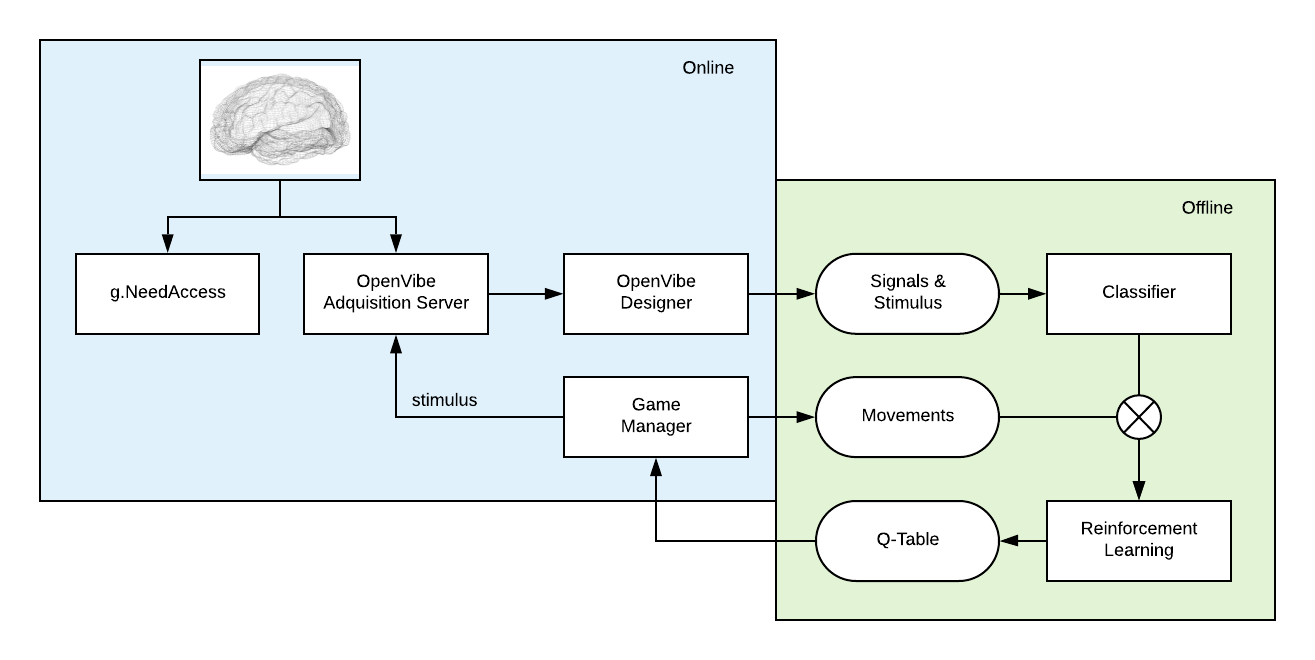
\includegraphics[width=\textwidth]{Images/complete_flow.png}
    \caption{Overview of the experimental procedure. Brainwaves are obtained by the OpenVibe Acquisition Server.  The Game Manager is responsible for generating the game screen, the game mechanics, and the game movements performed by the gaming agent.  It is also connected to the Acquisition Server to send stimulus information.  The captured information is stored by the OpenVibe Designer.  Offline, EEG signals are classified and they are linked to each game movement calculated by the Game Manager to determine proper rewards for each action.  This information is used by a Reinforcement Learning algorithm that iteratively trains a Q-Table in order to improve the performance of the agent that plays the game.}
    \label{diag:complete_flow}
\end{figure*}

\subsection{Brainwave Session}
\label{brainwavesession}

The retrieval of the OHC's brain activity, called the brainwave session, is one of the most critical parts of the study.  Subjects are recruited voluntarily and given a form with questions regarding their health (previous health issues and particular visual sensitivity), habits (sleeping hours, caffeine and alcohol consumption), and a written informed consent petition to collect the required data.  The experiment is conducted anonymously in accordance with the Declaration of Helsinki published by the World Health Organization. No monetary compensation is handed out. This study is approved by the Departamento de Investigación y Doctorado, Instituto Tecnológico de Buenos Aires (ITBA).  The brainwave sessions are performed with 8 subjects, 5 males and 3 females, with an average age of 25.12 years, a standard deviation of 1.54 years, and a range of 22-28 years. All subjects have normal vision, are right-handed and no history of neurological disorders.

After the form is filled out, a short description of the procedure is given to each subject. They are only told that the objective of the agent is to reach the goal and the four movements that the agent can make. When this concludes, the subject is introduced to the wireless digital EEG device (g.Nautilus, g.Tec, Austria) that she/he has to wear during the brainwave session. It has eight electrodes (g.LADYbird, g.Tec, Austria) on the positions Fz, Cz, Pz, Oz, P3, P4, PO7, and PO8, identified according to the 10-20 International System, with a reference set to the right ear lobe and ground set as the AFz position. The electrode contact points are adjusted applying conductive gel until the impedance values displayed by the program g.NeedAccess (g.Tec, Austria) are within the desired range. This process takes between 10 to 15 minutes. After this step, the subject is instructed to close their eyes, make eye movements and muscle chew in order to check the program and guarantee that the live channel values are accurate.

Once the headset is correctly applied, the OpenVibe Acquisition Server program, from the OpenVibe platform~\cite{OPEN-VIBE-PAPER}, is launched and configured with a sampling rate of $250$~Hz. A $50$~Hz notch filter is applied to filter out power line noise. An additional bandpass filter between $0.5$~Hz and $60$~Hz is applied. Data are handled and processed with the OpenVibe Designer, from the same platform, using 8 channels for the brain data (one channel per electrode) and an additional channel to record the stimulus, which corresponds to a game movement performed by the agent.  After everything is connected, the subject is seated in a comfortable chair in front of a computer screen. The brightness of the screen is set to the maximum setting to avoid any visual inconvenience in which the subject can not distinguish the components of the game that appear on the screen.

The Acquisition Server receives and synchronizes the signal data from the headset and any event information from the game, and transfers it to the OpenVibe Designer application. When the subject is ready, the Game Manager and the OpenVibe Designer programs are launched and configured to communicate with the previously mentioned Acquisition Server. A brainwave session consists of several matches, each one being a gameplay.  In the end, the sequence of game movements and the signal data generated for each match are saved for offline processing \footnote{The brainwave dataset has been published on the IEEE DataPort initiative~\cite{6emh-wb46-19}.}.

%ACA For each run, the signals and stimulus information are then passed to the classification module that uses them to train the classifier.  After this step is finished, the game movements and the trained classifier are used to update a Q-Table for each experience. Lastly, the calculated Q-Table is used to test if the agent has boosted its performance while playing the game. This module is explained in Section \ref{q_learning_step}.

\subsection{Cognitive Game Procedure}
\label{cognitive_experiment_details}
%This section details the game system characteristics, the brainwave session process and the retrieval and analysis of the generated data from the subjects interaction with the system.

\label{cognitive_experiment_system}{
The game parsimoniously consists of a $5x5$ grid of grey circular spots with a black background.  It is similar to the one proposed by~\cite{Iturrate2013}.  A blue spot indicates the current position of the agent and a green spot represents the goal, as shown in Figure  \ref{fig:game_representation}. The agent's objective is to reach the goal. The circular spot representing the goal remains static at the bottom-right position of the grid, while the one representing the position of the agent starts at the upper-left position of the grid and moves in each iteration.  When the agent reaches the goal, the position where the agent and the goal are located turns red, showing that the match has ended. There are four possible movements that the agent can perform: it can go upwards, downwards, towards the left and the right, and those movements are bounded to avoid the agent from leaving the grid. The movement direction is selected randomly and is executed once every 2 seconds.  After each gameplay, there is a pause of 5 seconds until the next match starts. Each time an agent moves, the Game Manager program sends an event marker to the Acquisition Server.  This is considered a stimulus to the observational human critic.  The game is designed as to be evident whenever there is an error (i.e. the agent moves away from the objective) so the subject can notice it immediately after the stimulus is presented, possibly triggering the expected cognitive response, which can be imprinted as an ErrP component within the EEG stream.

\begin{figure}[h!]
\begin{subfigure}{0.5\textwidth}
\centering
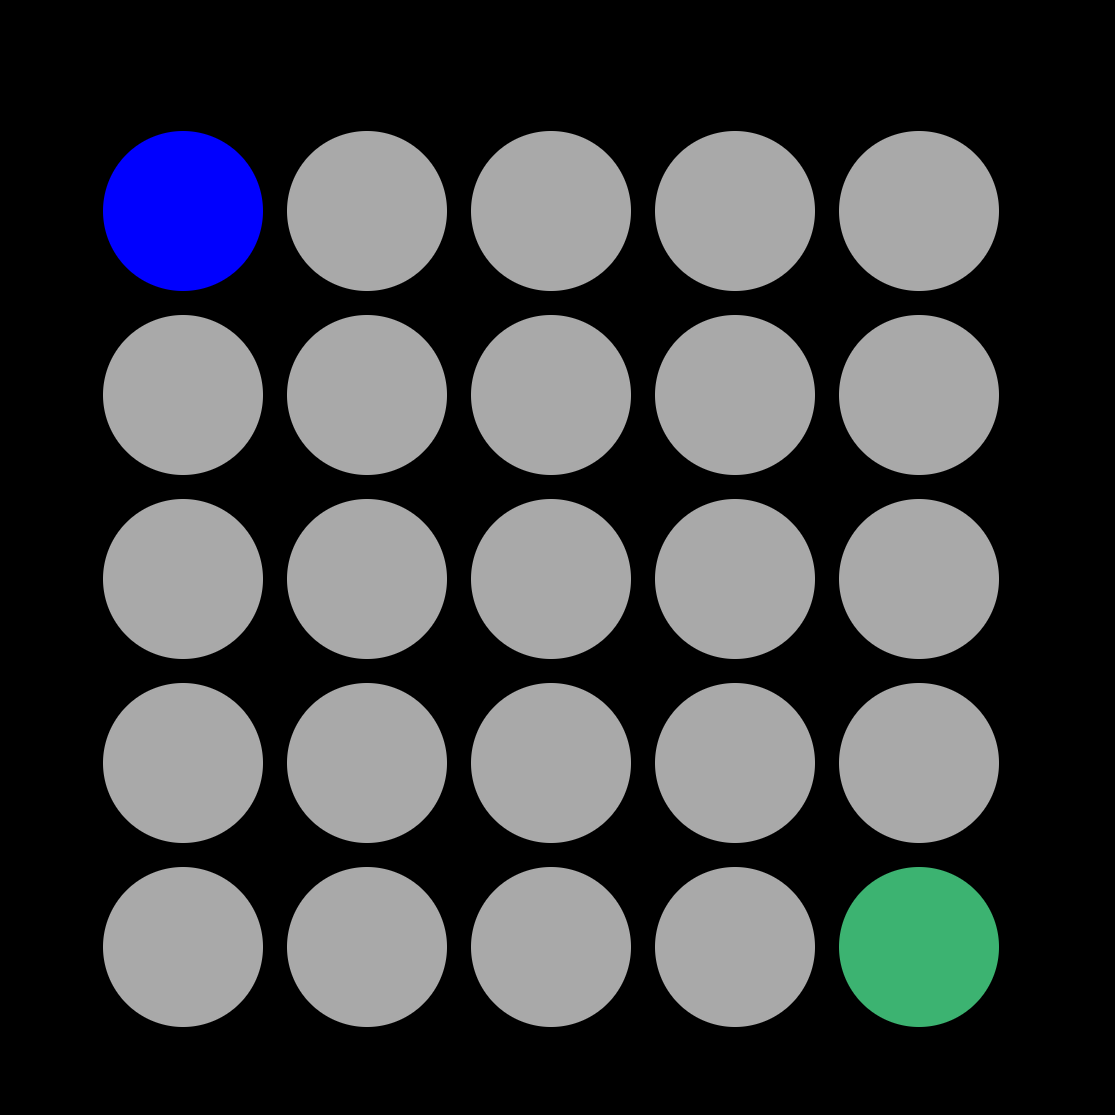
\includegraphics[scale=0.2]{Images/grid_initial_state.png}
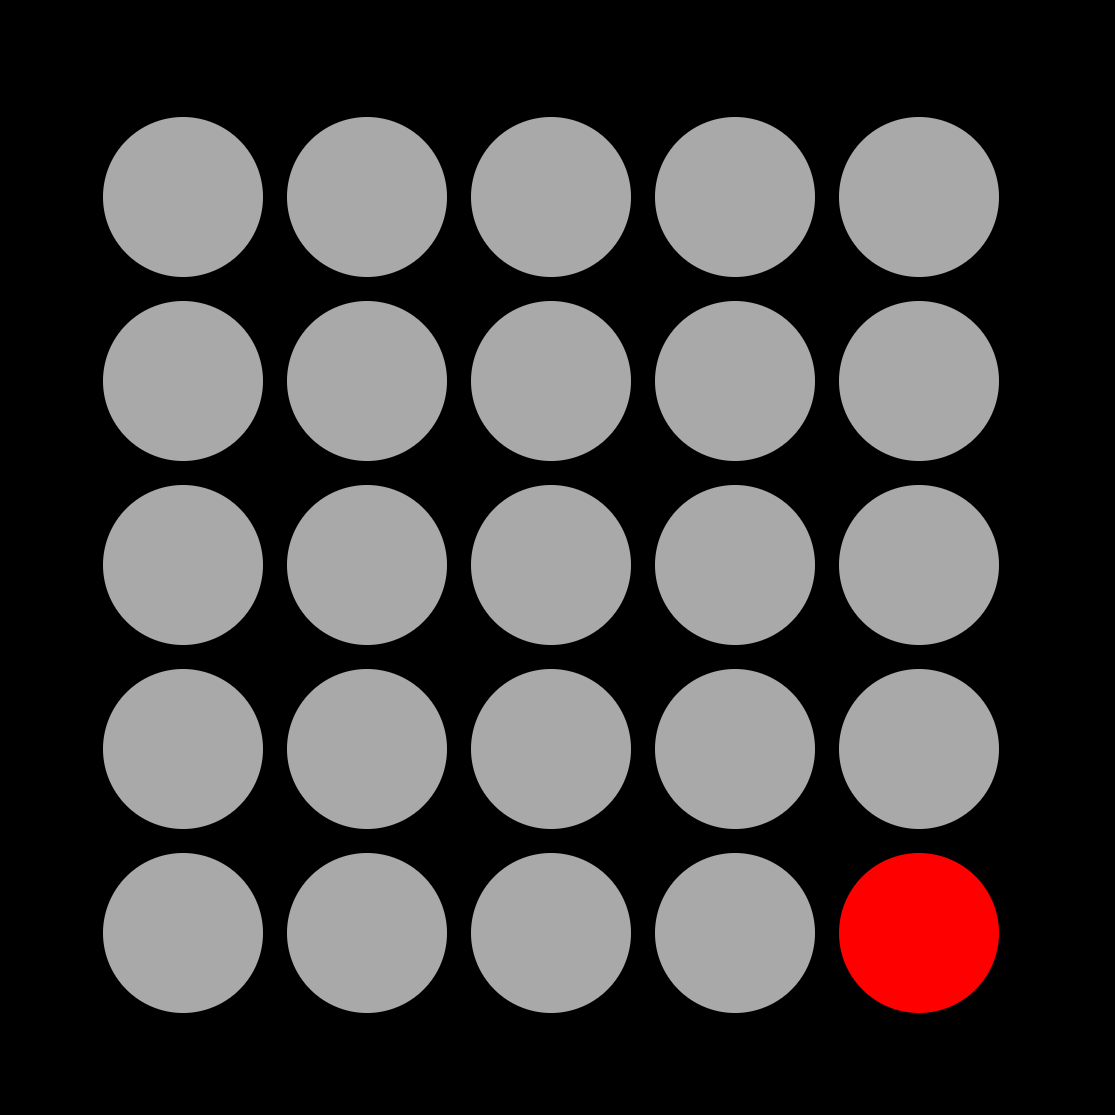
\includegraphics[scale=0.2]{Images/grid_end_state.png}
\end{subfigure}
\centering
\caption{Grid system representation used in the cognitive game. The blue spot represents the initial location while the green spot represents the target location. Once the agent reaches the target spot, its color turns red to indicate the end of the play.}
\label{fig:game_representation}
\end{figure}

%\section{Calibration}
%\label{section:calibration}

%The first step in order to be able to find ErrP signals is to choose the most efficient algorithm, and the proper calibration. In order to do this different parameters are tested for a set of algorithms and for each individual subject. Initially a sub-selection of experiments is used to define a subset of parameters to test with, and then all the data are tested with this subset of parameters.

\subsection{Signal Processing, Segmentation and Classification}
\label{section:calibration}

To aid the detection of the ErrP response, an offline processing pipeline and classifier is constructed to identify whether the action taken by the agent is an error or not, from the human observer's point of view. It is developed in Python using the "MNE" software platform \cite{MNE-PYTHON}, which is a package designed specifically for processing EEG and Magnetoencephalography data, and built upon the machine learning library Scikit-Learn~\cite{scikit-learn}.

This pipeline consists of the offline processing of the collected signals used to train a classifier that can decide whether an error potential is triggered. Firstly, the output of a brainwave session is read and an additional band-pass filter of 0.1-20.0 Hz is applied to the signal. Samples that correspond to the start of an event are tagged using the data from the stimulus channel.

After the raw data are loaded and tagged, epochs are extracted. Epochs consist of all the sample points that take place during the 2 seconds from the start of the event, 2 seconds corresponding to the time it takes for each action to take place, resulting in 500 samples per channel, as the sampling frequency is 250 Hz. Thus, each epoch is composed of a matrix $500$ x $8$ channels.

Samples that do not correspond to an epoch (located beyond the 2 seconds frame after the onset of the event) are not used. Also, epochs referring to the start or finish of each match are excluded.

In this way, the raw data of a brainwave session is processed into an array of matches where each element is an array of epochs tagged with a number specifying the prediction of the classifier, i.e. if the epoch corresponds to an action that made the agent move further from the goal (hit) or an action that made the agent moves closer to the goal (no-hit). The ErrP is expected to be found in hits. To get the data ready for classification, the stimulus channel is removed to classify the signals using only the EEG data. Each epoch is regularized using a MinMaxScaler, i.e. subtracting the minimum value in the epoch and dividing by the signal peak-to-peak amplitude~\cite{Zhou2019}.  The eight channels are concatenated using the MNE Vectorizer function, which transforms the data matrix into a single array sample. Lastly, this data are used by the classification module as information to train and test a classifier. Five different classification algorithms are used:  Logistic Regression, Multilayer Perceptron with a hidden layer of 100 neurons (i.e. default values for the Scikit-Learn MLPClassifier), Random Forest, KNeighbours with k=3 and finally a linear kernel Support Vector Classifier (i.e. SVM)~\cite{Lotte2018}.

%Vectorized epochs are used in the final classification step.

%and finally the logistic regression classifier.  Even tough the classification accuracy is low, the information is enough to have valid rewards that can be used to retrieve the information.

%a classifier is trained for each subject and then epochs from their experiences are classified. These classifications are then used by a reinforcement learning algorithm to train the agent. This last algorithm is explained in detail in section \ref{q_learning_step}.

\subsection{Reinforcement Learning}
\label{learning}

Each match consists of a list of game movement configurations and the associated epochs obtained from OHC's brainwaves.  The set of matches of each OHC is split into training and testing.  Training matches are used to train the classifier to identify the ErrP signal.  After a classifier is trained, the epochs extracted from the test matches are classified as hit or no-hit.  A reward for each movement in the match is generated based on the prediction from the classifier for that movement.  The reward can either be -1 when the event is classified as a hit or 0 when it is classified as a no-hit. The accuracy of these rewards depends on the performance of the classifier. The list of game movements and their associated reward information is used to train the agent by a variant of Reinforcement Learning called Q-Learning algorithm.

%The set of experiences of each subject is split into training and testing, so that the results of the classification can then be used to improve the performance of the agent. Each experience includes an ordered list of extracted epochs for each movement that the agent carried out plus the game state information, i.e. the movement specification.

%After a classifier is trained, the epochs of the experience are classified as hit or no-hit.  With the game state information and the classification of the test data of an experience, a reward file is composed. This file specifies a reward for each movement in the game run, based on the classification of the event that corresponds to that movement. The reward can either be -1 when the event is classified as a hit or 0 when it is classified as a no-hit. The accuracy of this rewards depends on the performance of the classifier. This reward file is used by the a variant of a Reinforcement Learning algorithm called Q-Learning algorithm.


\subsection{Q-Learning}{
\label{q_learning_step}

Q-Learning~\cite{Watkins1992} is a form of model-free reinforcement learning, where an agent tries an action at a particular state and evaluates its consequences in terms of the reward or penalty it receives.  To represent rewards, a matrix $Q(s,a)$ is used, where rows correspond to all the possible states, and columns represent all possible actions.  This matrix is known as the Q-Table.  The algorithm proceeds by randomly choosing what action to do and iteratively updating the Q-Table based on the received reward $r$ by the following equation

\begin{equation}
    Q(s,a) \leftarrow Q(s,a) + \alpha[r+\gamma* \max_{\tilde{a}} Q(\tilde{s}, \tilde{a})-Q(s, a) ]
    \label{equ:update_q_table}
\end{equation}

\noindent where $s$ is the current state, $a$ the action, $\alpha$ the learning rate and $\gamma$ the discount factor, a value between 0 and 1 that determines the importance of long term results versus immediate rewards.  Hence, $Q(s,a)$ is the expected value of the sum of discounted rewards that the agent will receive if in the $s$ state, it takes the action $a$ according to this policy.  Once the environment has been extensively explored and the Q-Table has been optimized, the action chosen for a given state is the one that maximizes the expected reward according to the Q-Table matrix.

The algorithm is developed in Python and uses the OpenAI Gym toolkit~\cite{openai}. Gym is a toolkit for developing and comparing reinforcement learning algorithms. It makes no assumptions about the structure of an agent, and is compatible with any numerical computation library, such as TensorFlow or Theano~\cite{tensorflow2015-whitepaper}.

\subsection{Gaming Agent Learning Procedure}
\label{q_learning_step_alg}

The gaming agent learning procedure uses the testing matches from brainwave sessions produced during the cognitive game procedure phase, and their components are schematized in Figure~\ref{diag:complete_flow}.

This phase is divided into a sequence of run sessions and a gaming agent training match.  During the run session, the agent plays 200 matches guided by a specific Q-Table with a 5\% chance of randomly selecting a movement, to reduce deadlocks and loops.  Following the run session, the agent performs a single gaming agent training match.  The gaming agent starts first with a Q-Table initialized with zeros, so the initial policy for the agent is randomized.  For the agent to learn from the feedback generated by the OHC, movement actions are determined by the reply of the agent's actions that were taken during one brainwave session match, in an offline reinforcement learning scheme~\cite{Levine2020}. This allows the Q-Table to be built based on the OHC's feedback from the movements the agent took, which were executed pseudo-randomly during the brainwave session.  The previously mentioned feedback is not explicit as it comes from the interpreted brain signal data. This implies that the reward is determined by the OHC's brain activity.

Hence, following the iterative procedure based on Equation~\ref{equ:update_q_table}, the Q-Table is updated in each gaming agent training match. After the algorithm finishes replicating all the steps from the brainwave session match, the Q-Table is stored and used by the agent in the next run session.


\section{Results}
\label{results}


\begin{figure}[ht]
    \centering
    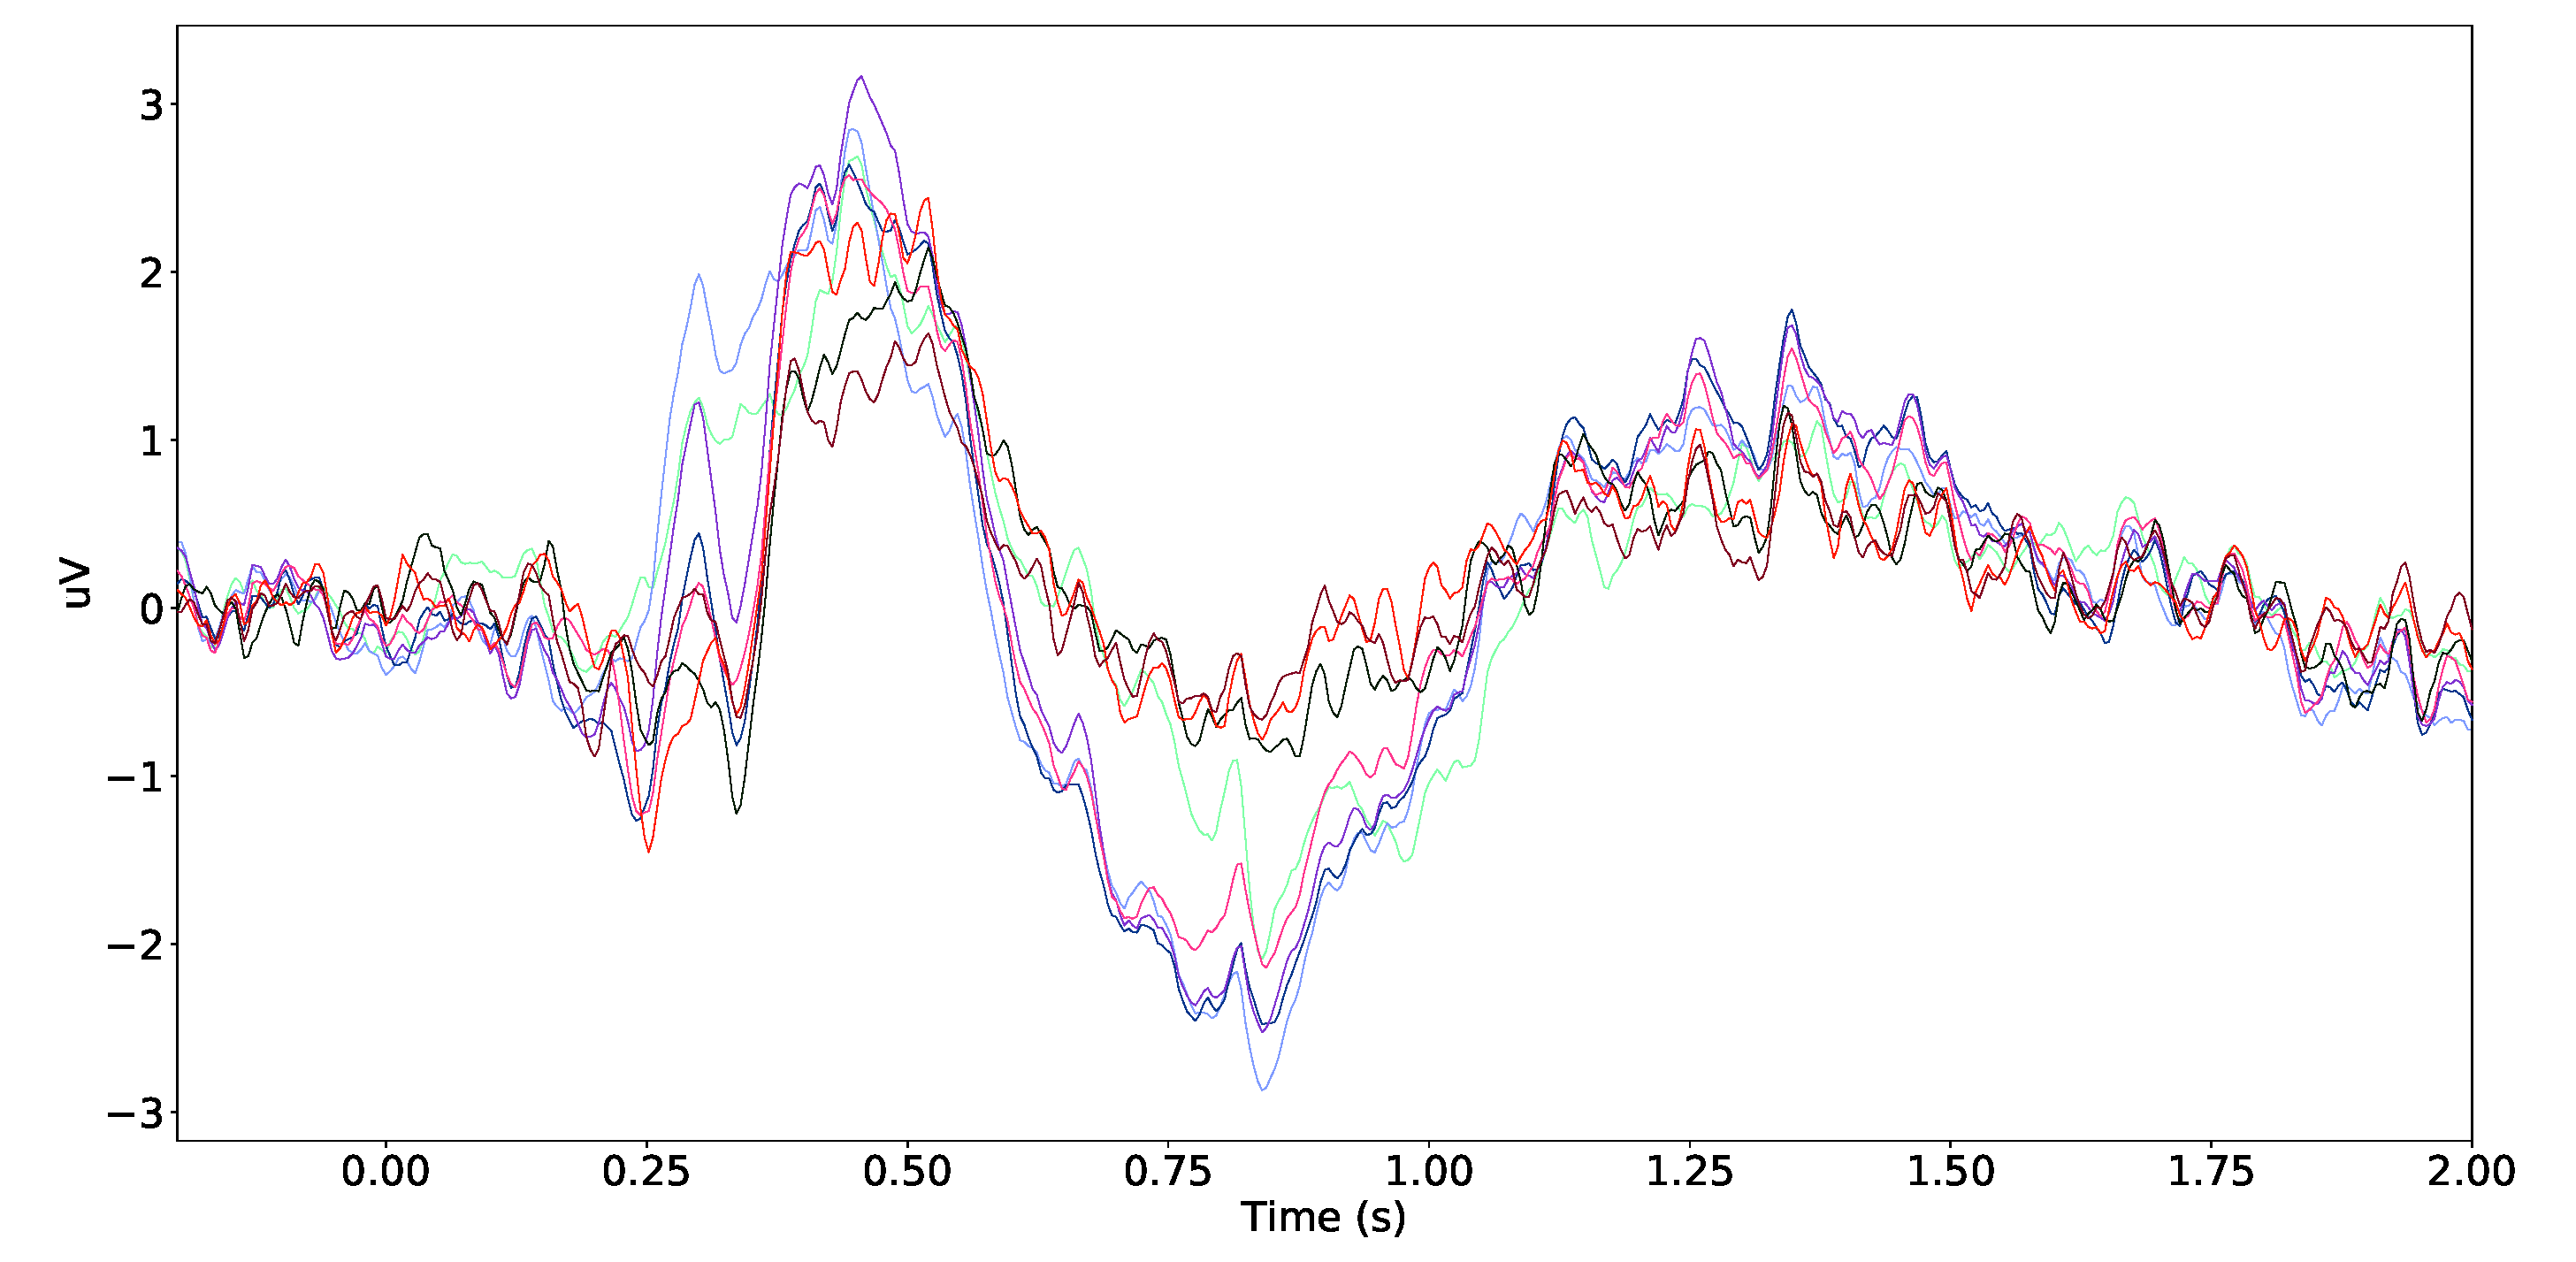
\includegraphics[width=0.5\textwidth]{revisedimages/avg_closer.eps}
    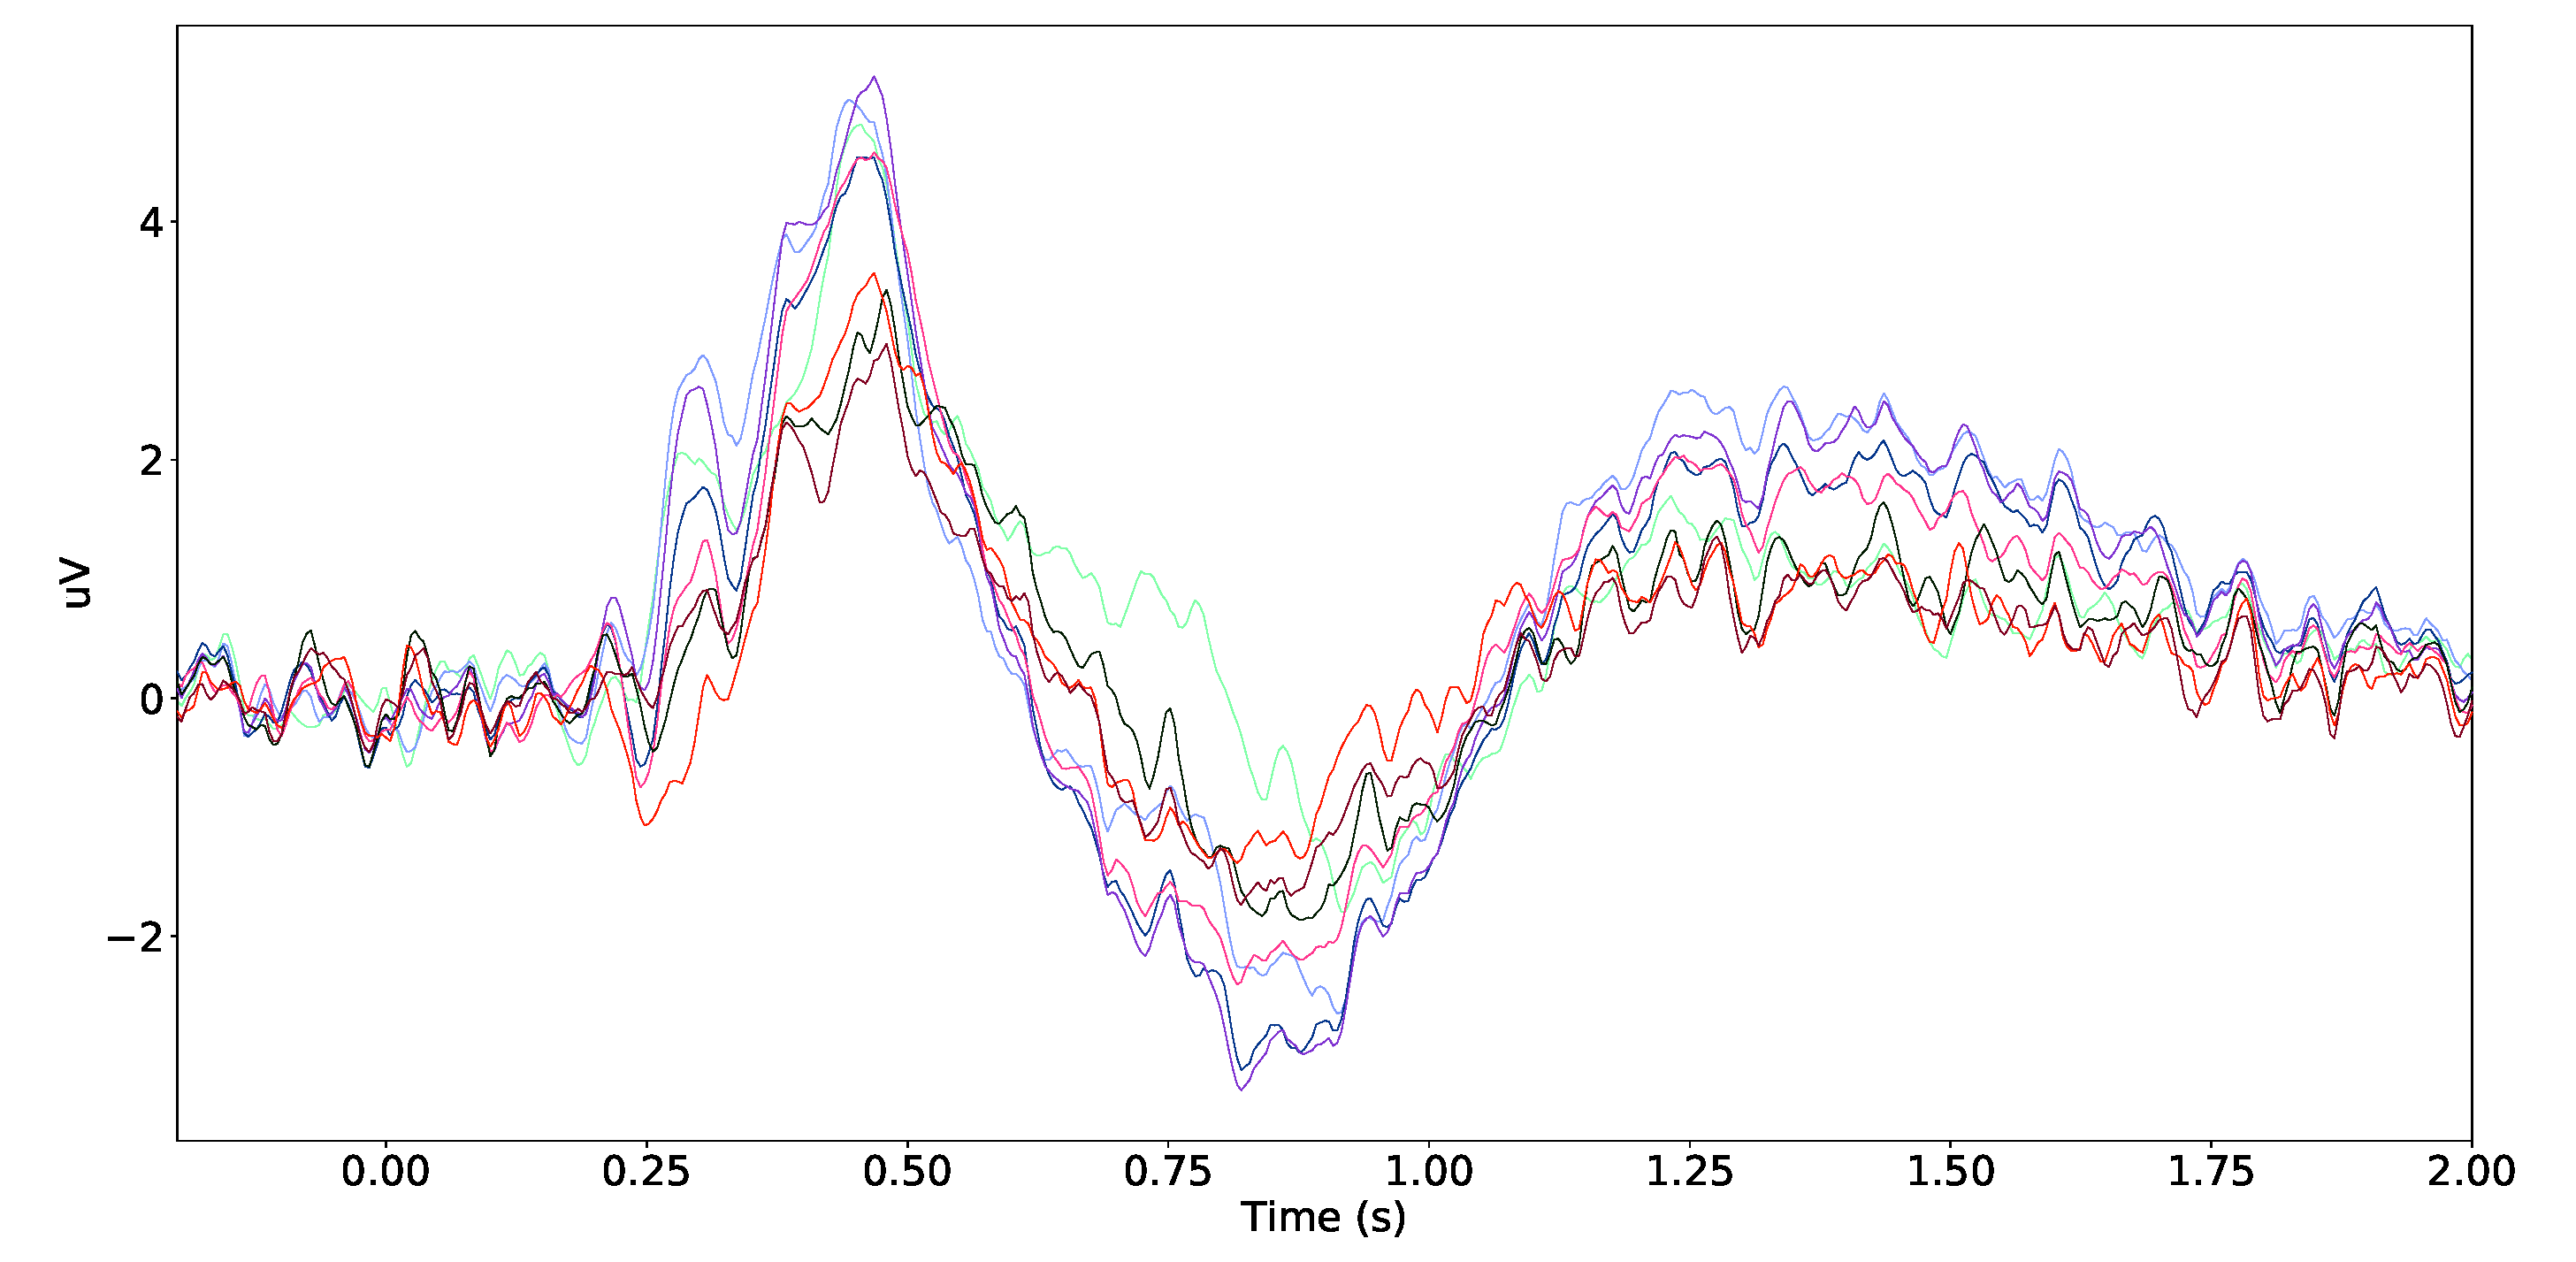
\includegraphics[width=0.5\textwidth]{revisedimages/avg_further.eps}
    \caption{Grand Average for all OHCs for the closer and further condition.  It can be seen the bump around 300 ms.}
    \label{fig:classifiers}
\end{figure}

Figure~\ref{fig:classifiers} shows the binary classification accuracy obtained for the eight OHCs using five different classification algorithms and using a 10-fold cross-validation procedure.  The best overall performance is obtained using Logistic Regression.  In addition, the classification accuracy obtained averaging 5 epochs is shown as well.  Although the signal averaging procedure improves the Signal-To-Noise-Radio (SNR) of the ErrP response, it reduces the number of data samples, producing a clear improvement only for the OHCs that contain more samples (1, 3 and 7).

\begin{figure}[ht]
    \centering
    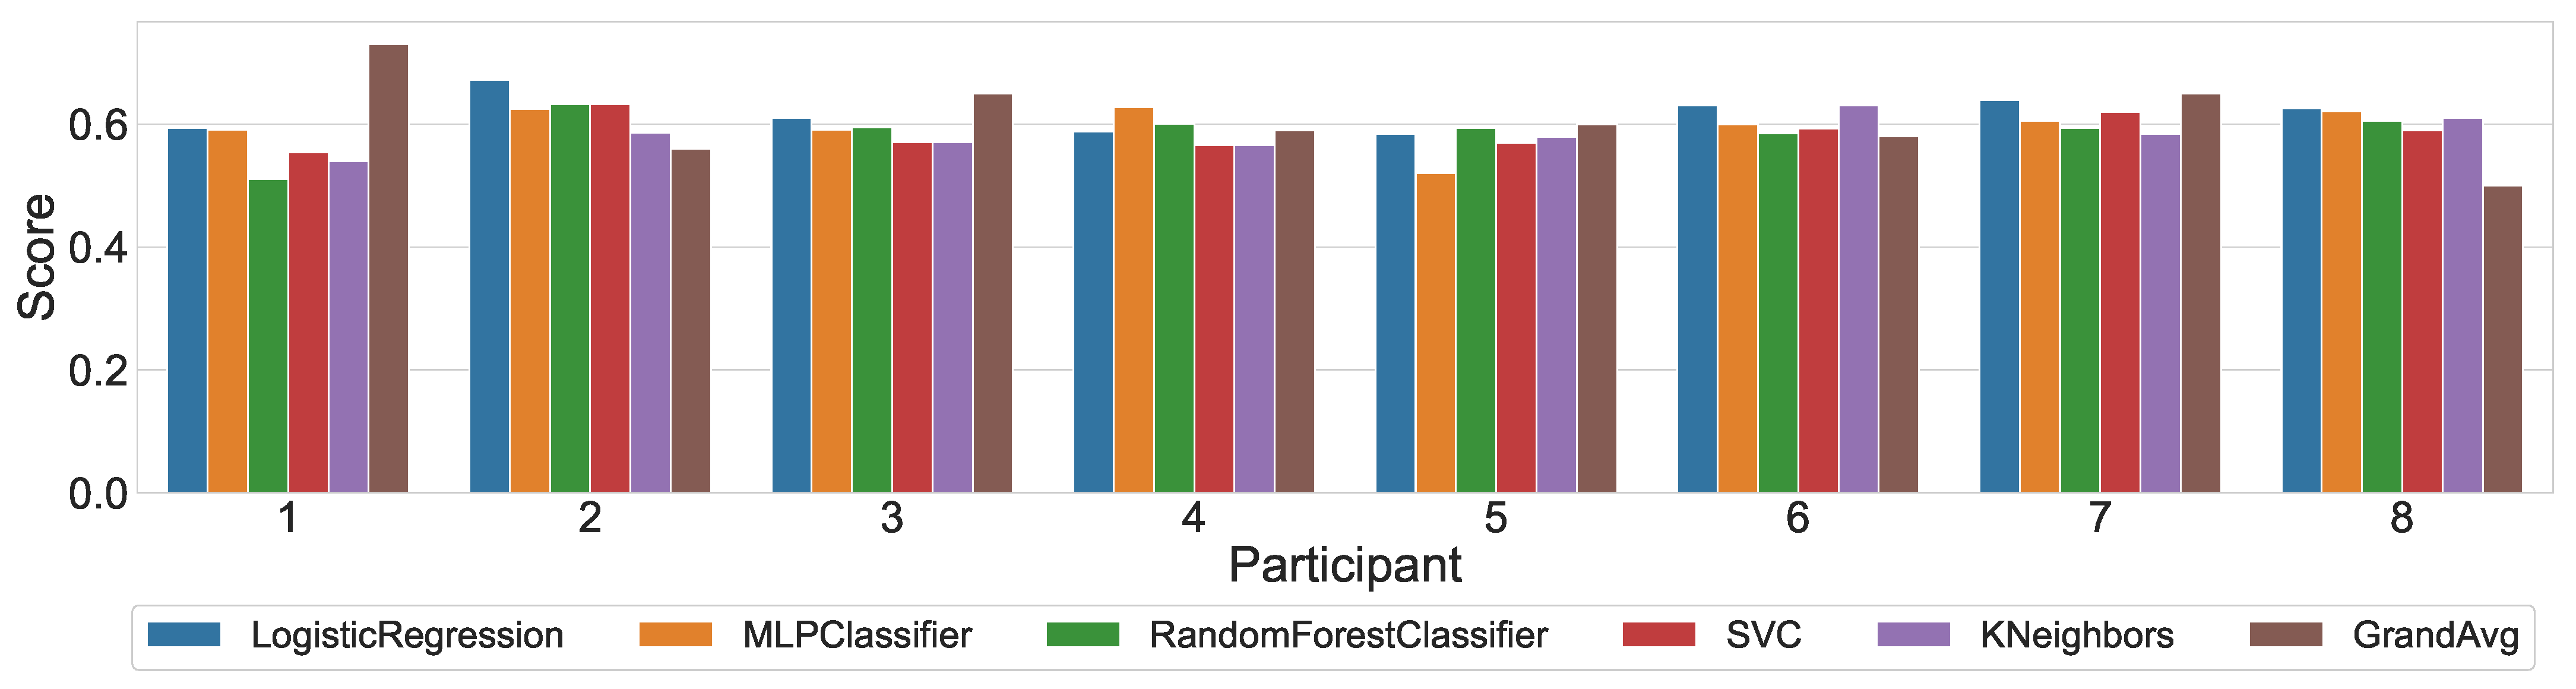
\includegraphics[scale=0.11]{revisedimages/cross_val.eps}
    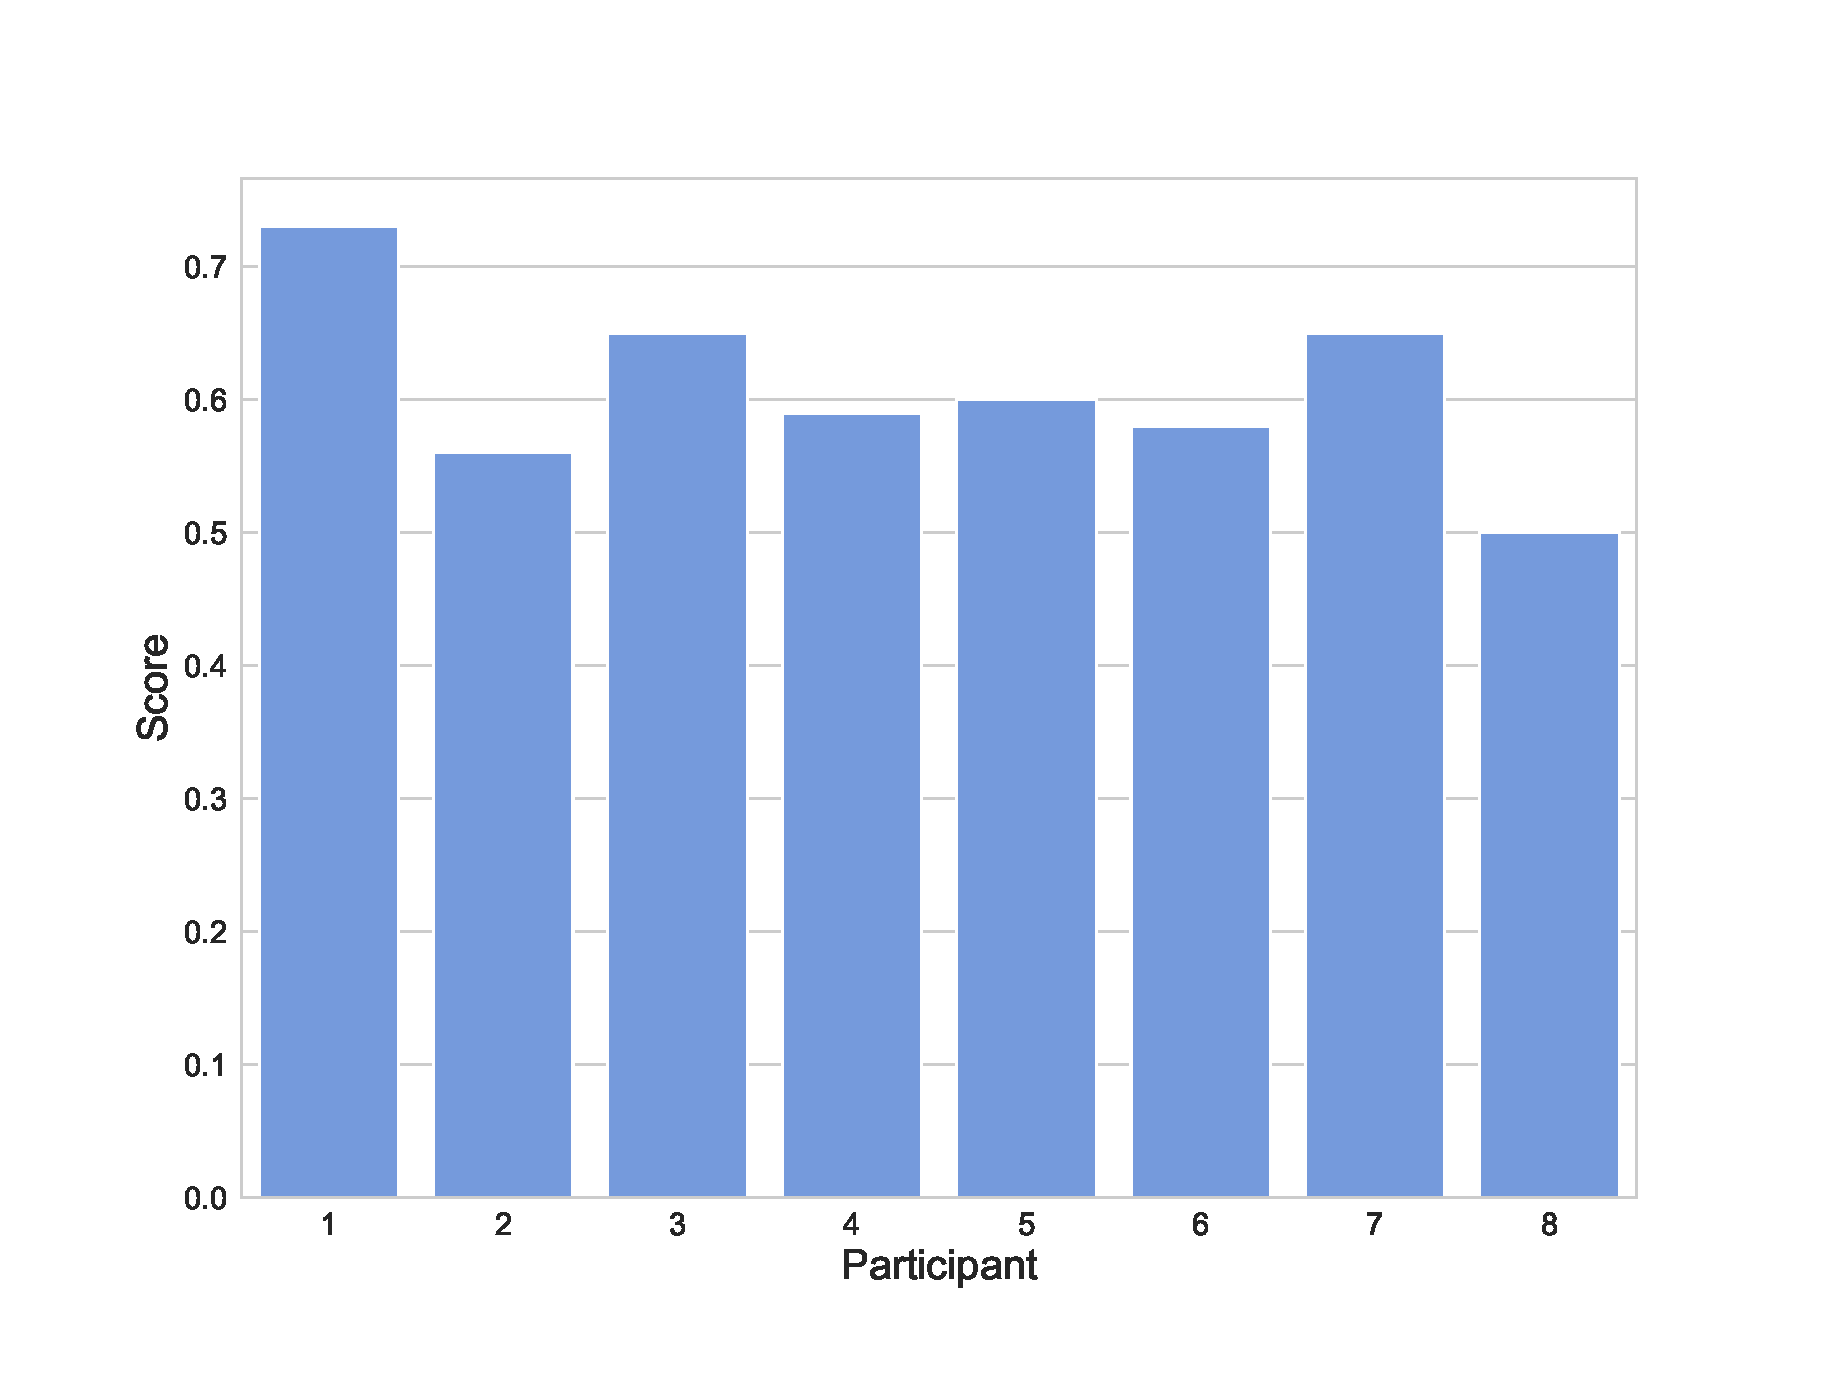
\includegraphics[scale=0.21]{revisedimages/avg_5_segments.eps}
    \caption{Binary single trial classification score using five different classifiers while recognizing ErrP potentials for the eight OHCs.  The classification score using an ensemble average of 5 epochs is shown as well (GrandAvg). Chance Level is 0.5.}
    \label{fig:classifiers}
\end{figure}


On the other hand, Figure \ref{fig:avg_steps} shows the average amount of steps it takes for the agent to reach the goal for each OHC, as the Q-Table is progressively trained using the reward information obtained from the prediction of the trained classifier. Each point corresponds to a run session where the average number of steps for the agent to reach the goal using a specific Q-Table is specified, for 200 repetitions. The first point, at the x-value 0, represents the number of steps the agent takes to reach the goal with an untrained Q-Table, where movements are decided randomly. The next point corresponds to the amount of steps it takes to reach the goal using a policy derived from a Q-Table trained after one brainwave session match, and so on.

\begin{figure}[h!]
\begin{subfigure}{0.5\textwidth}
\centering
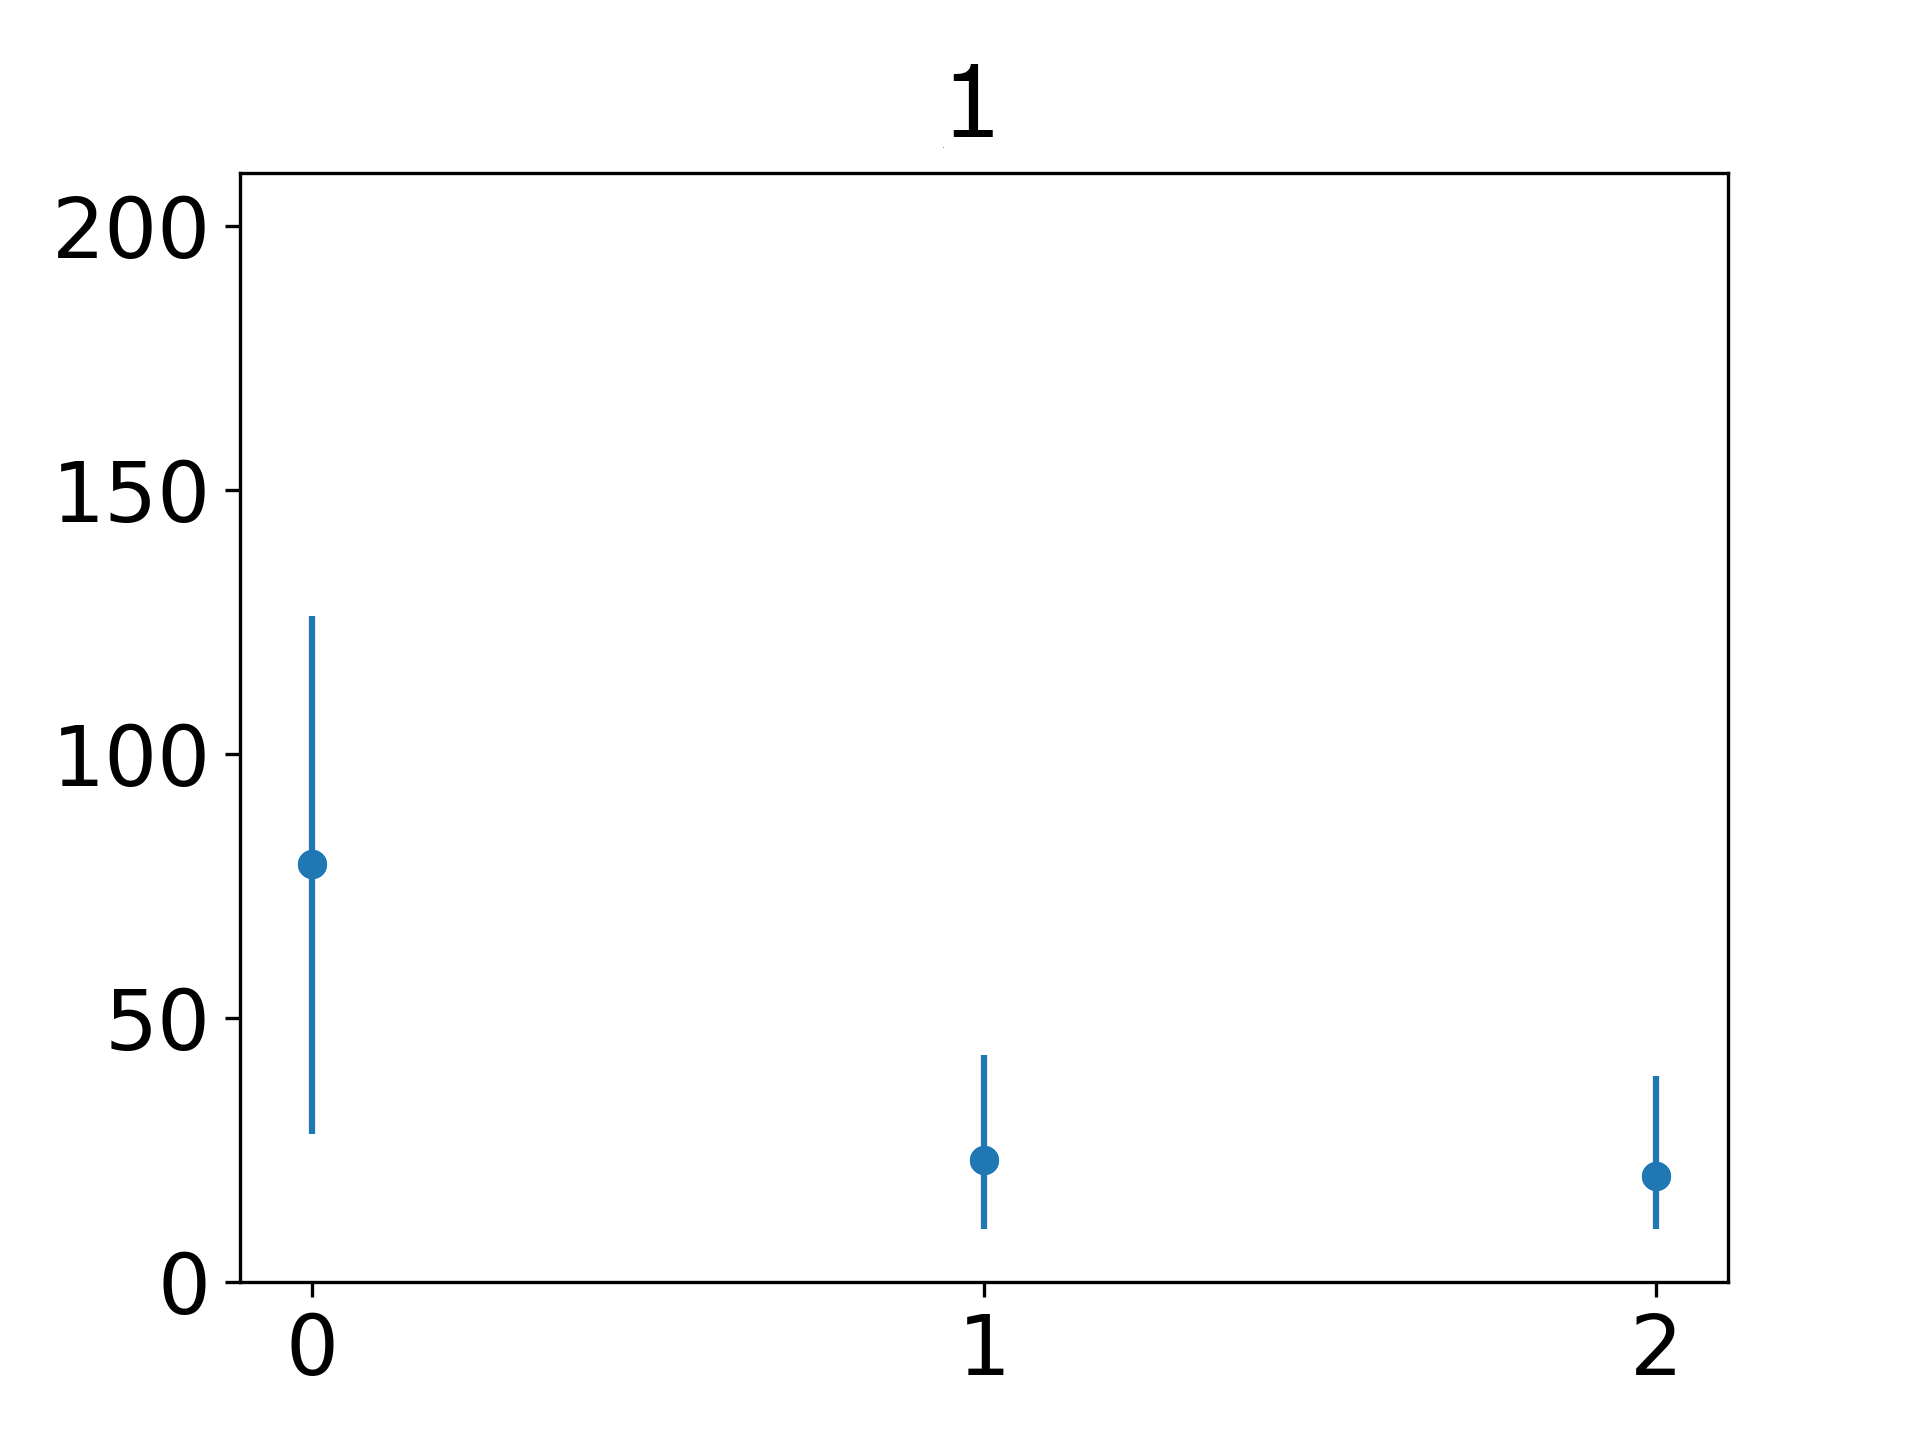
\includegraphics[scale=0.27]{Images/Average_steps/a.png}
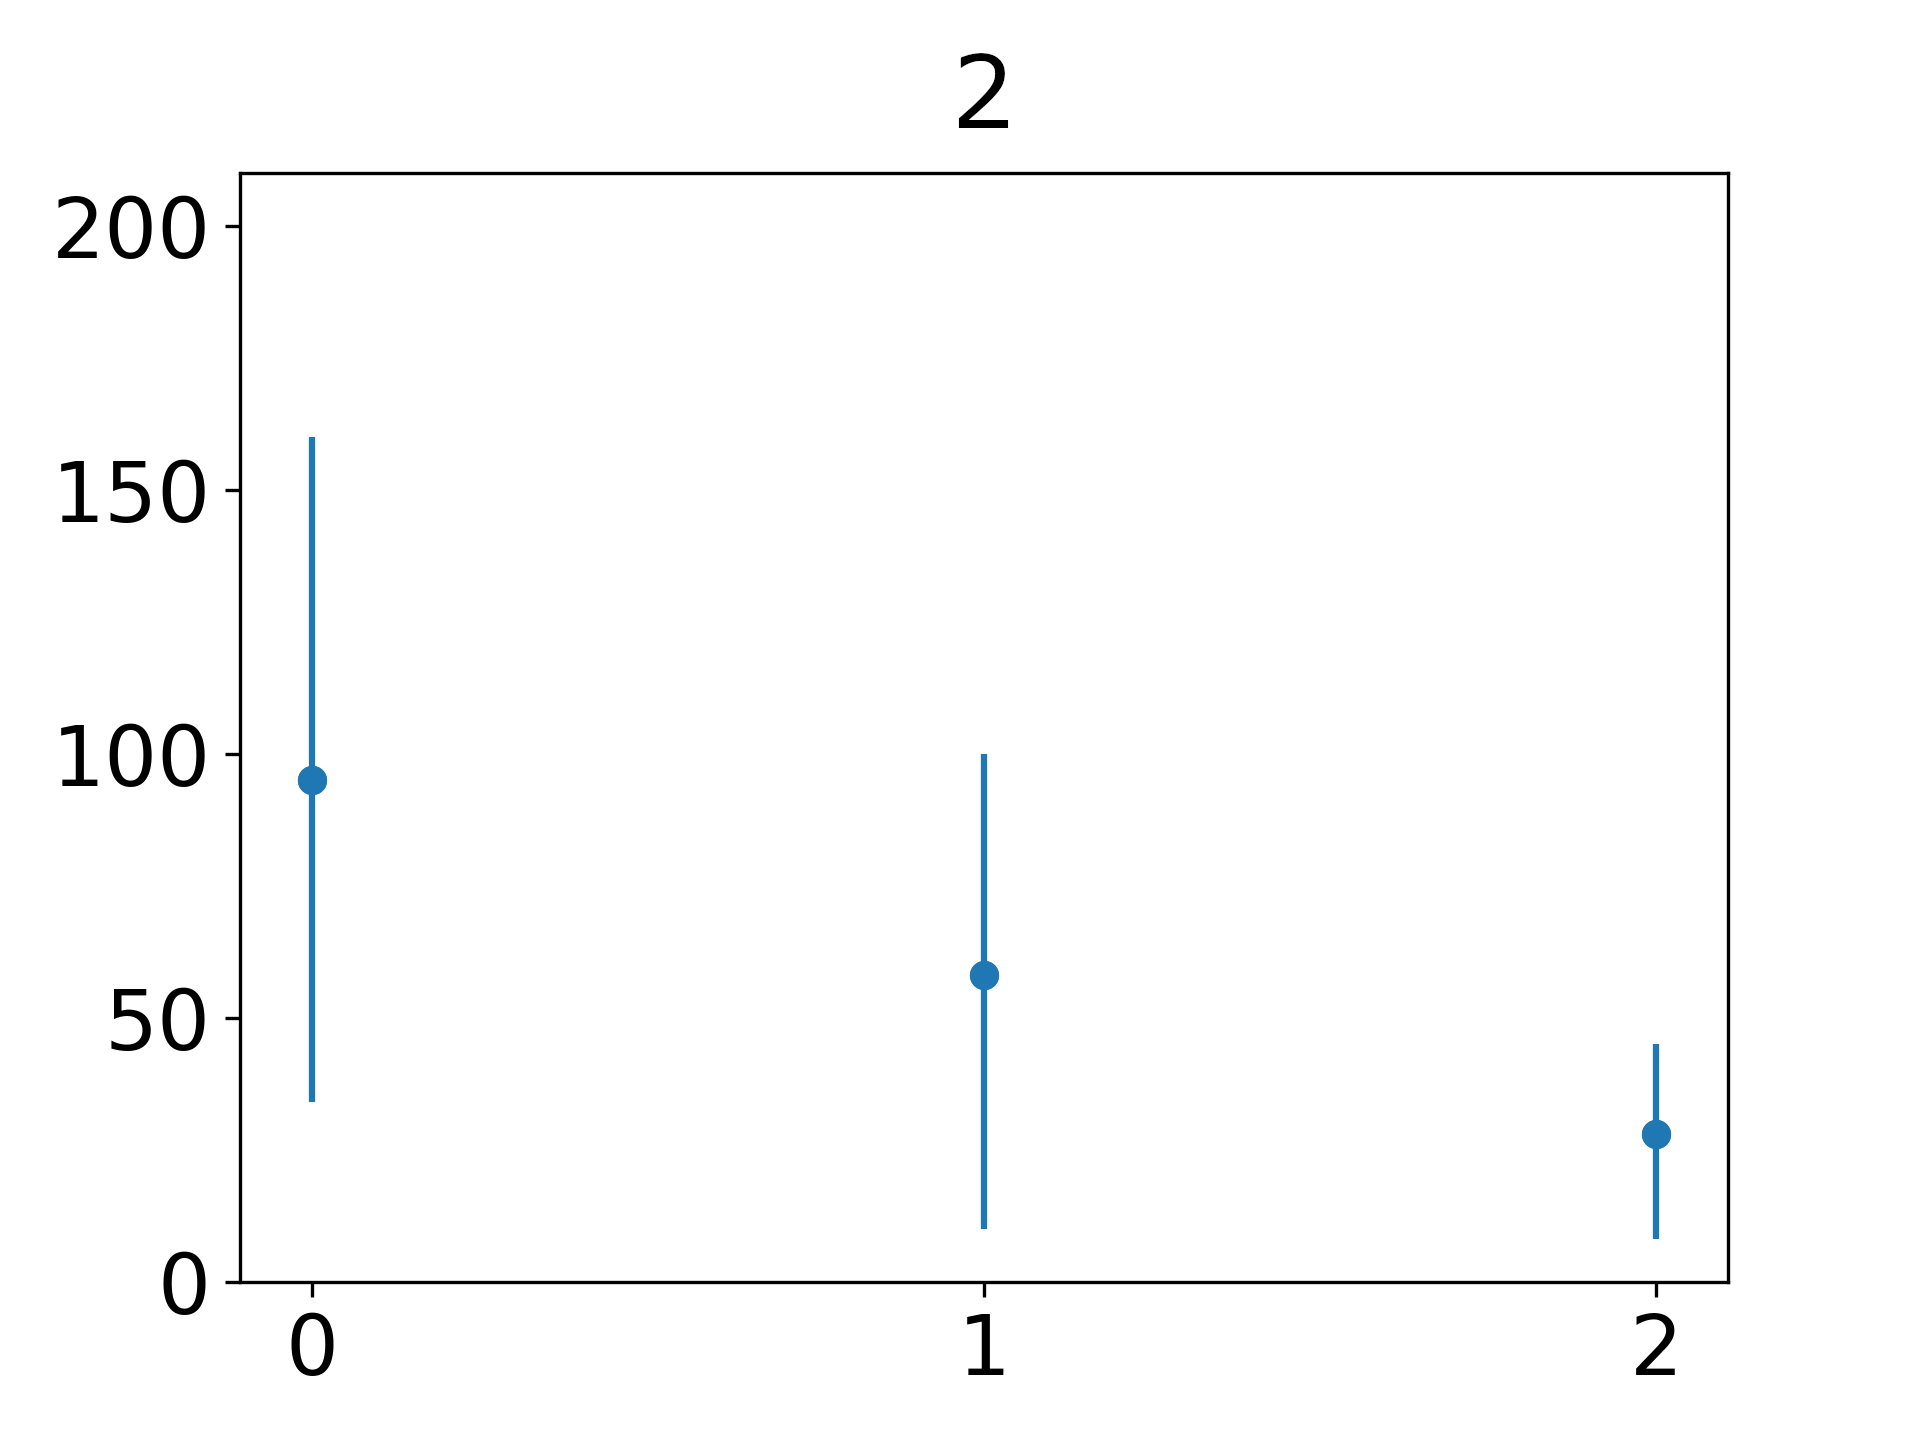
\includegraphics[scale=0.27]{Images/Average_steps/b.png}
\centering
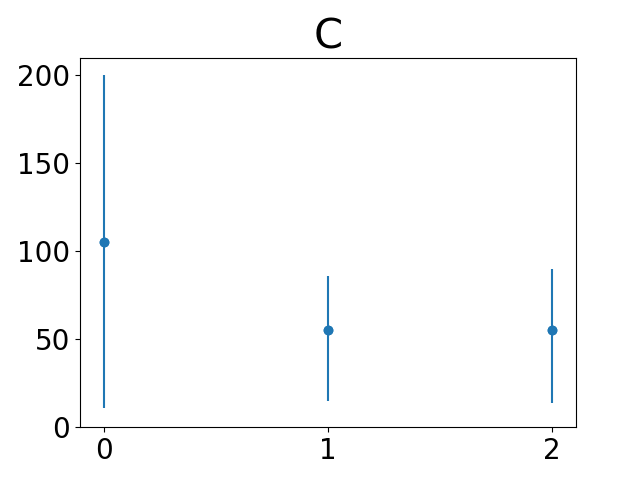
\includegraphics[scale=0.27]{Images/Average_steps/c.png}
 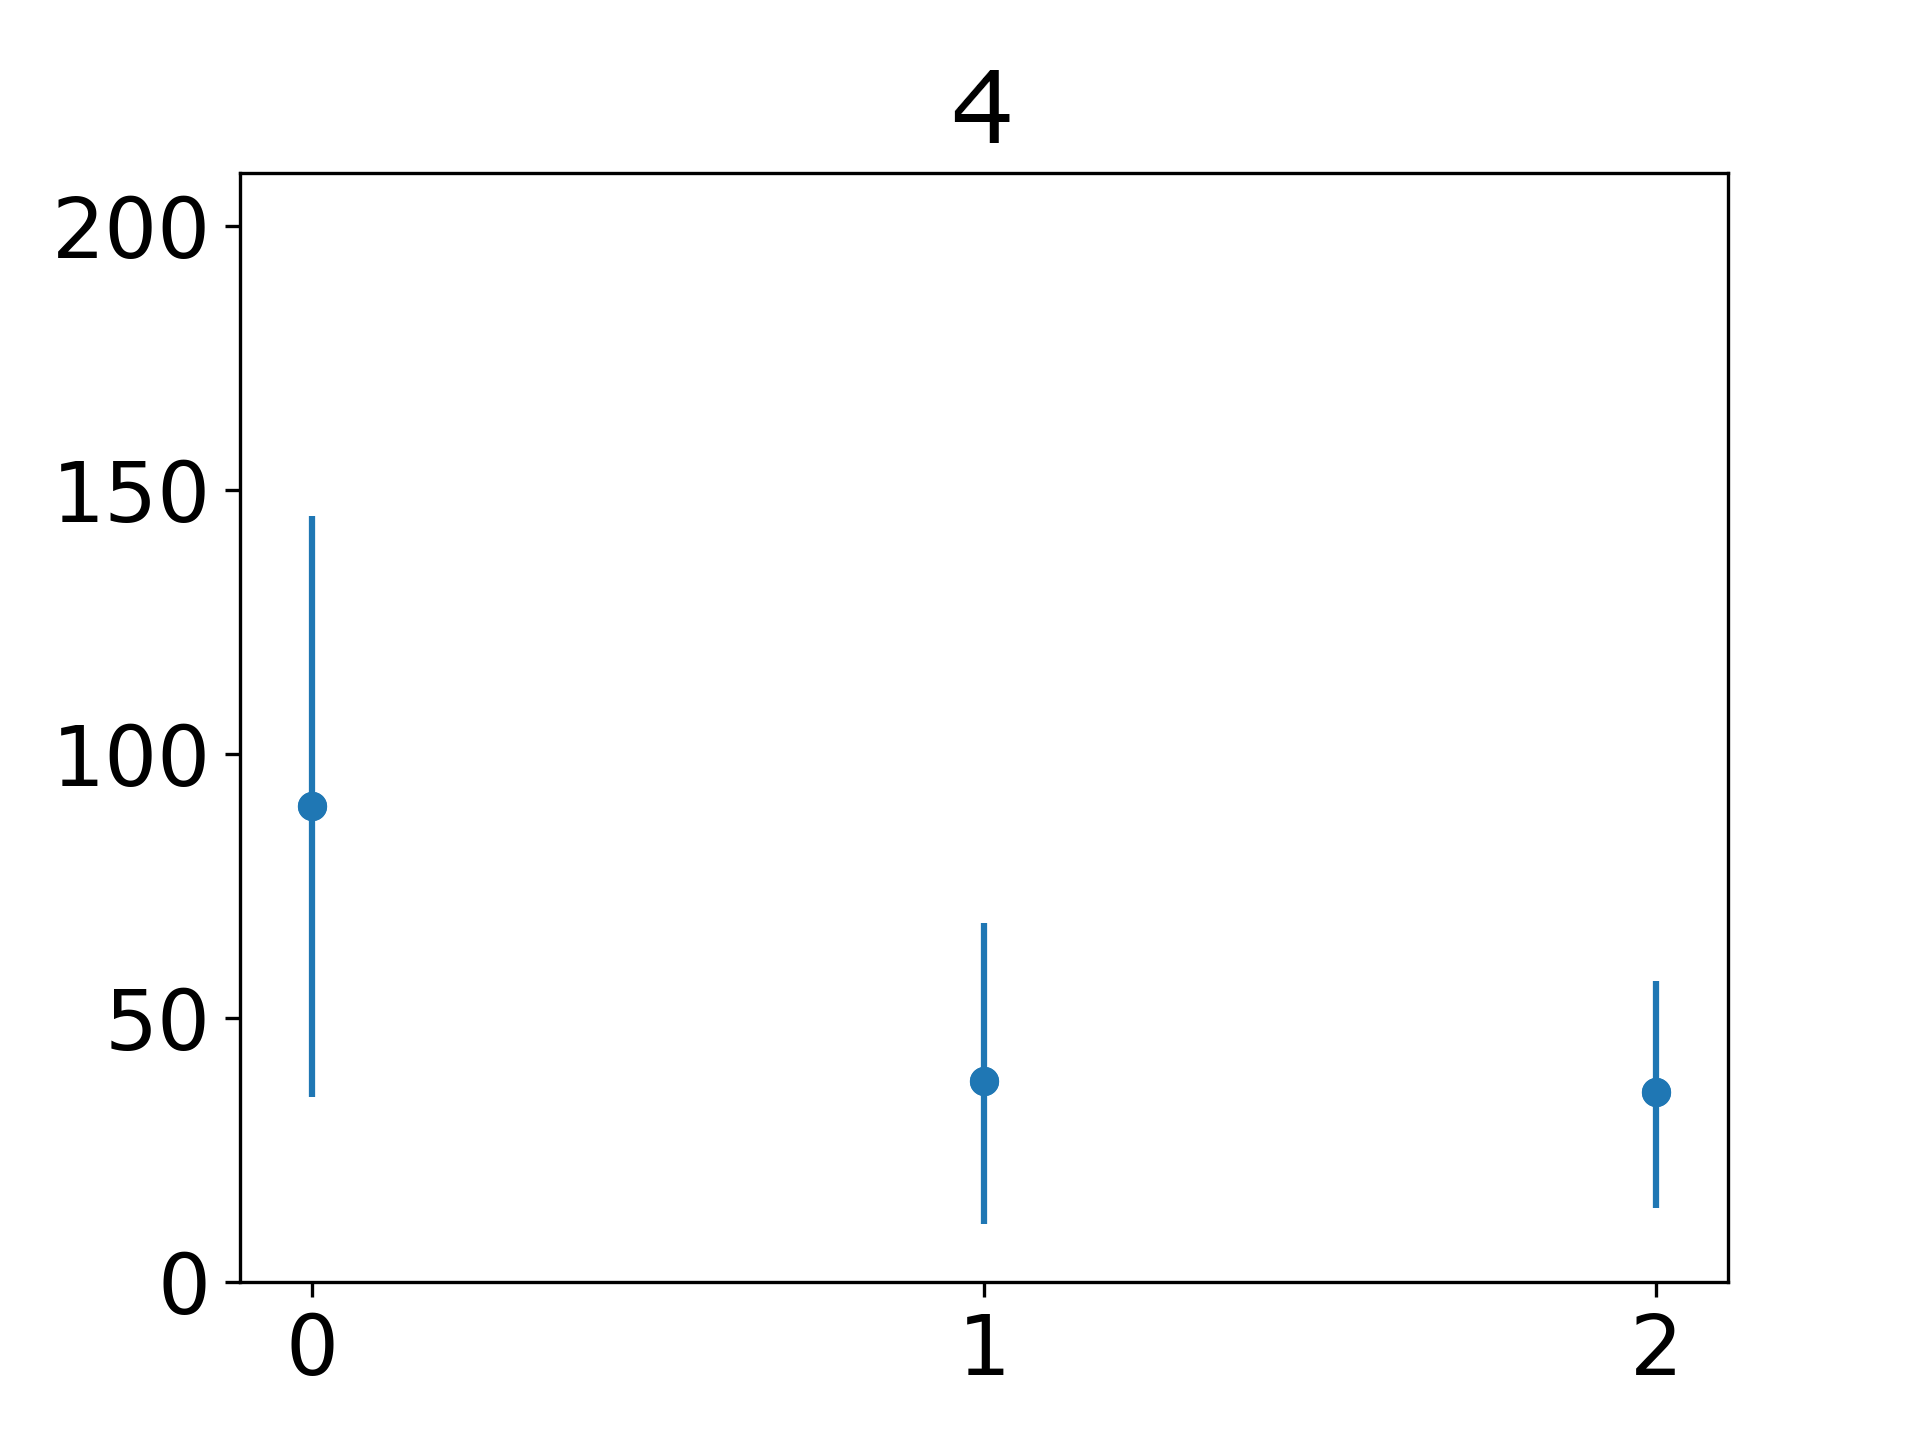
\includegraphics[scale=0.27]{Images/Average_steps/d.png}
 \centering
  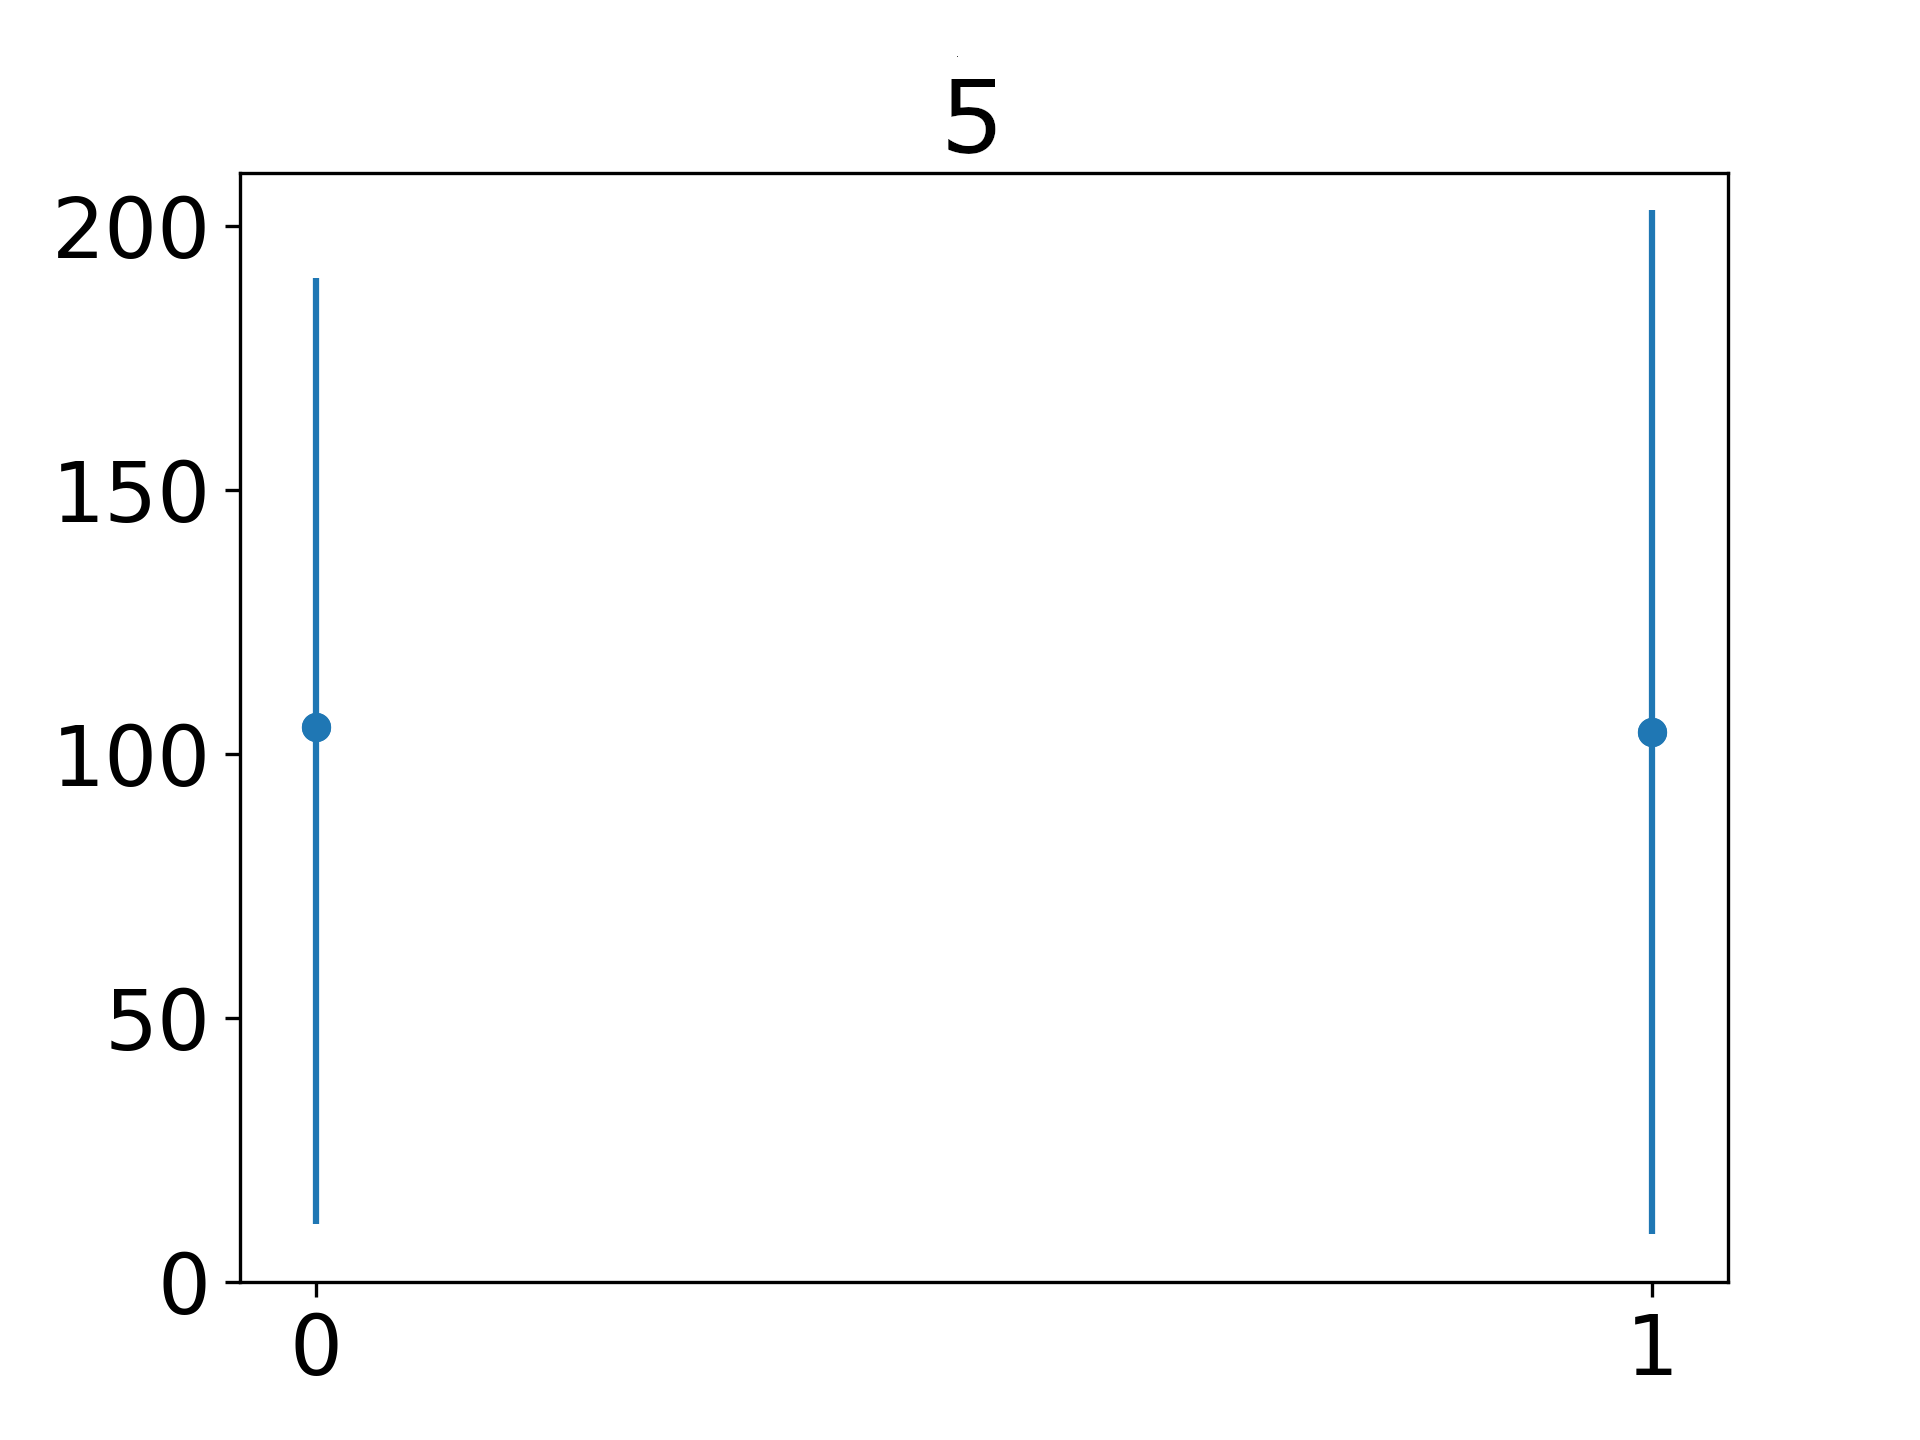
\includegraphics[scale=0.27]{Images/Average_steps/e.png}
  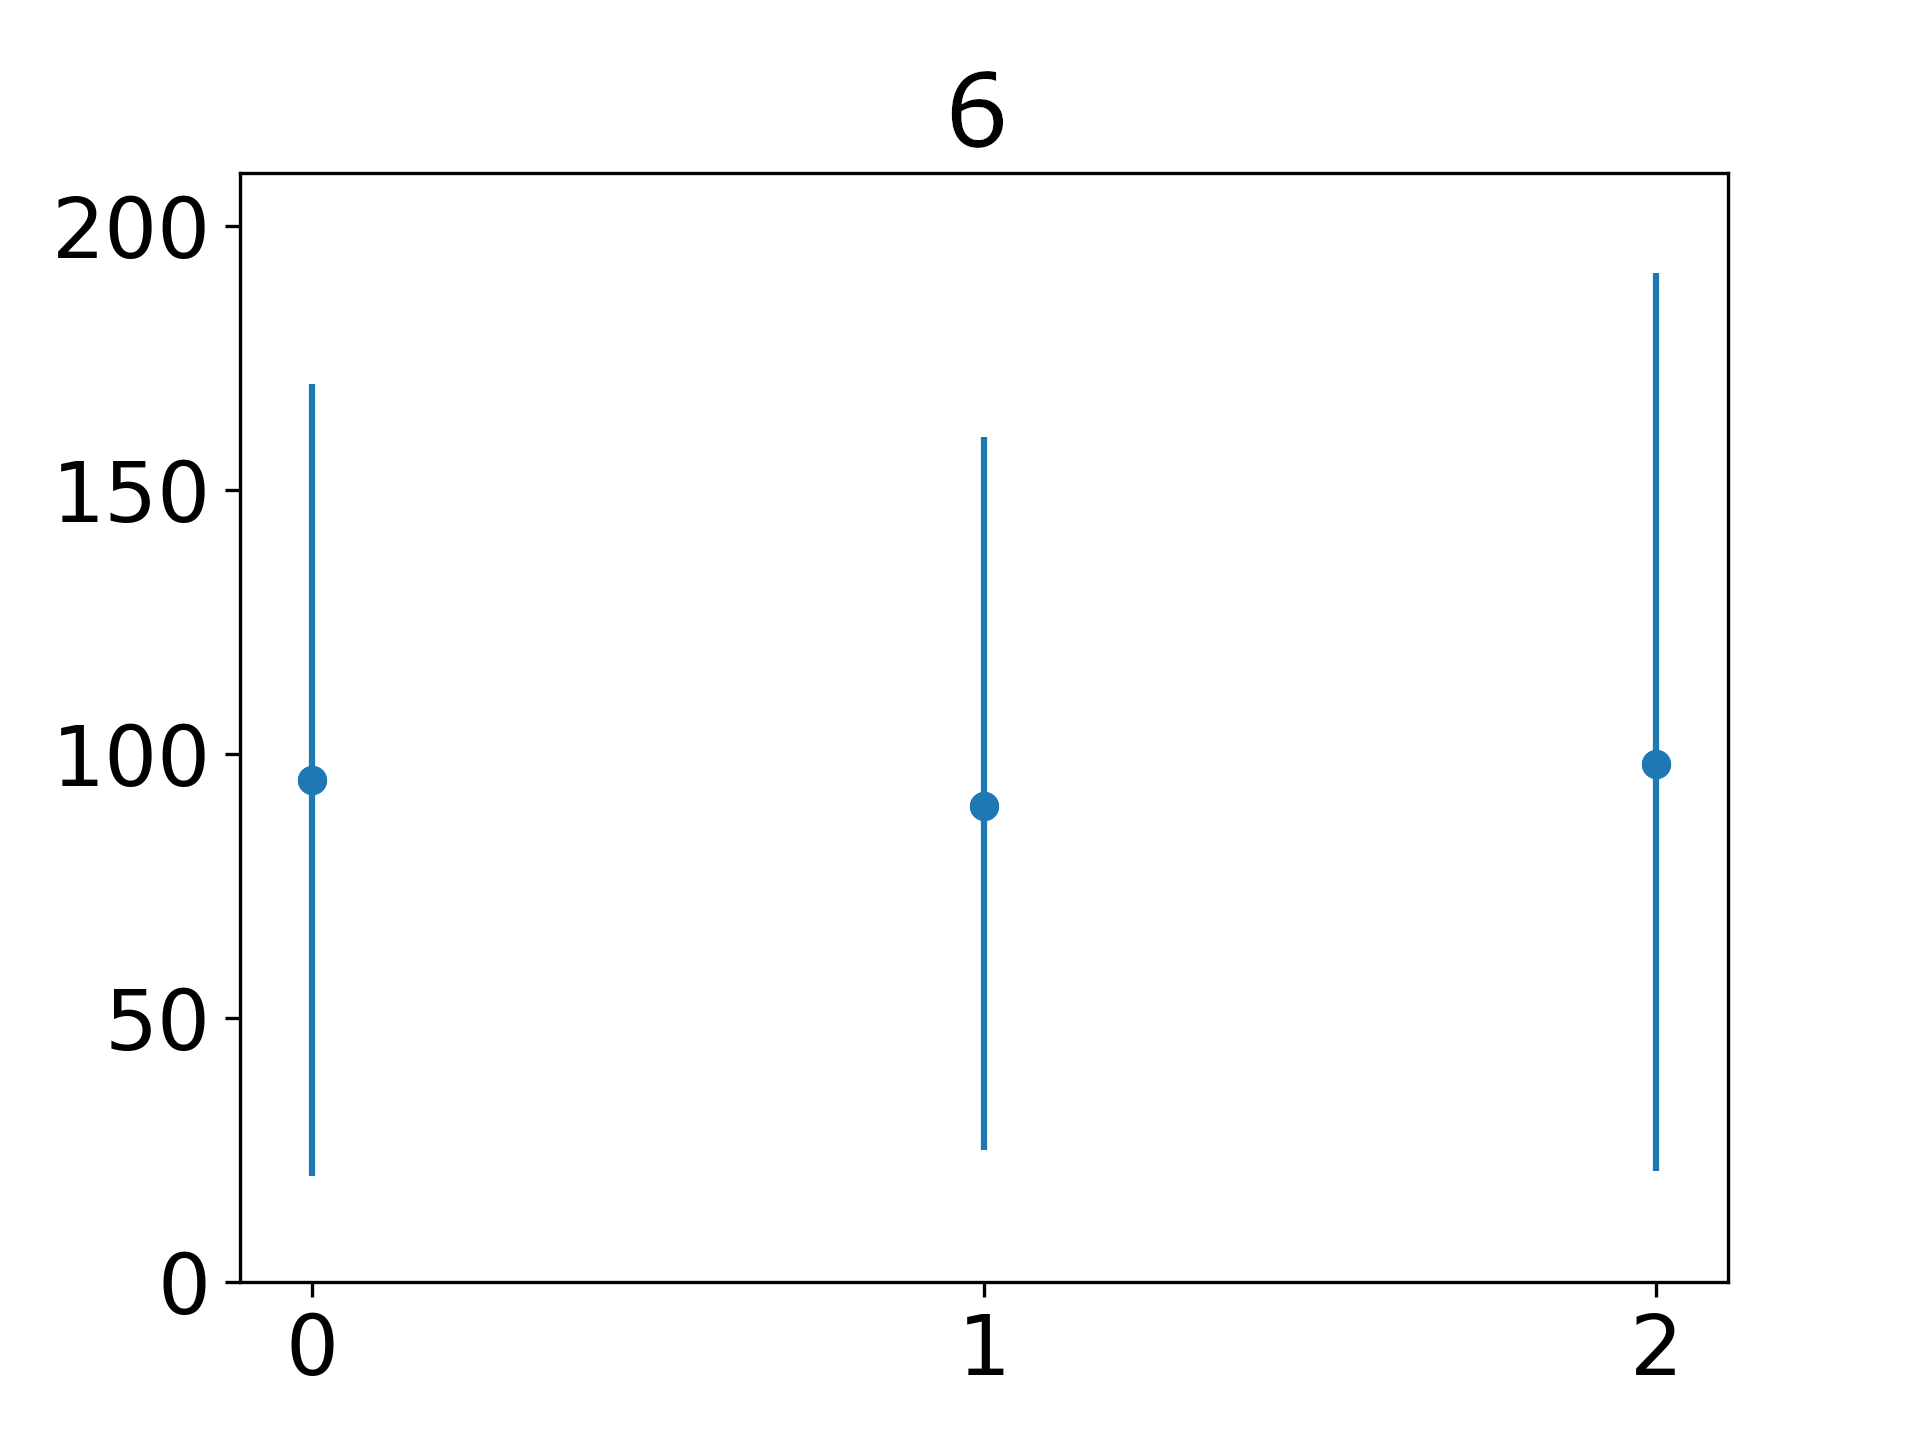
\includegraphics[scale=0.27]{Images/Average_steps/f.png}
  \centering
  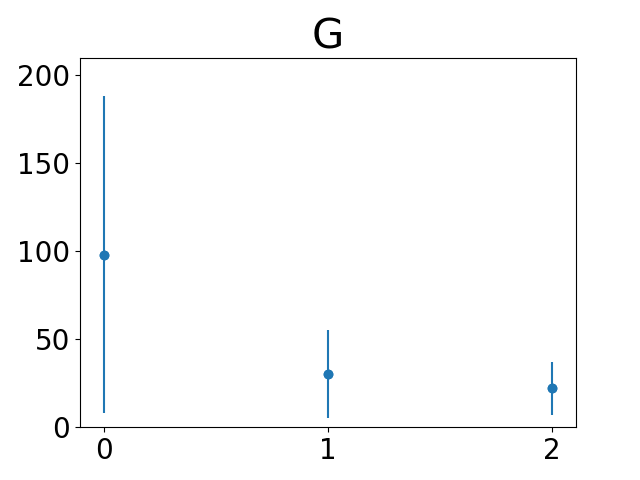
\includegraphics[scale=0.27]{Images/Average_steps/g.png}
  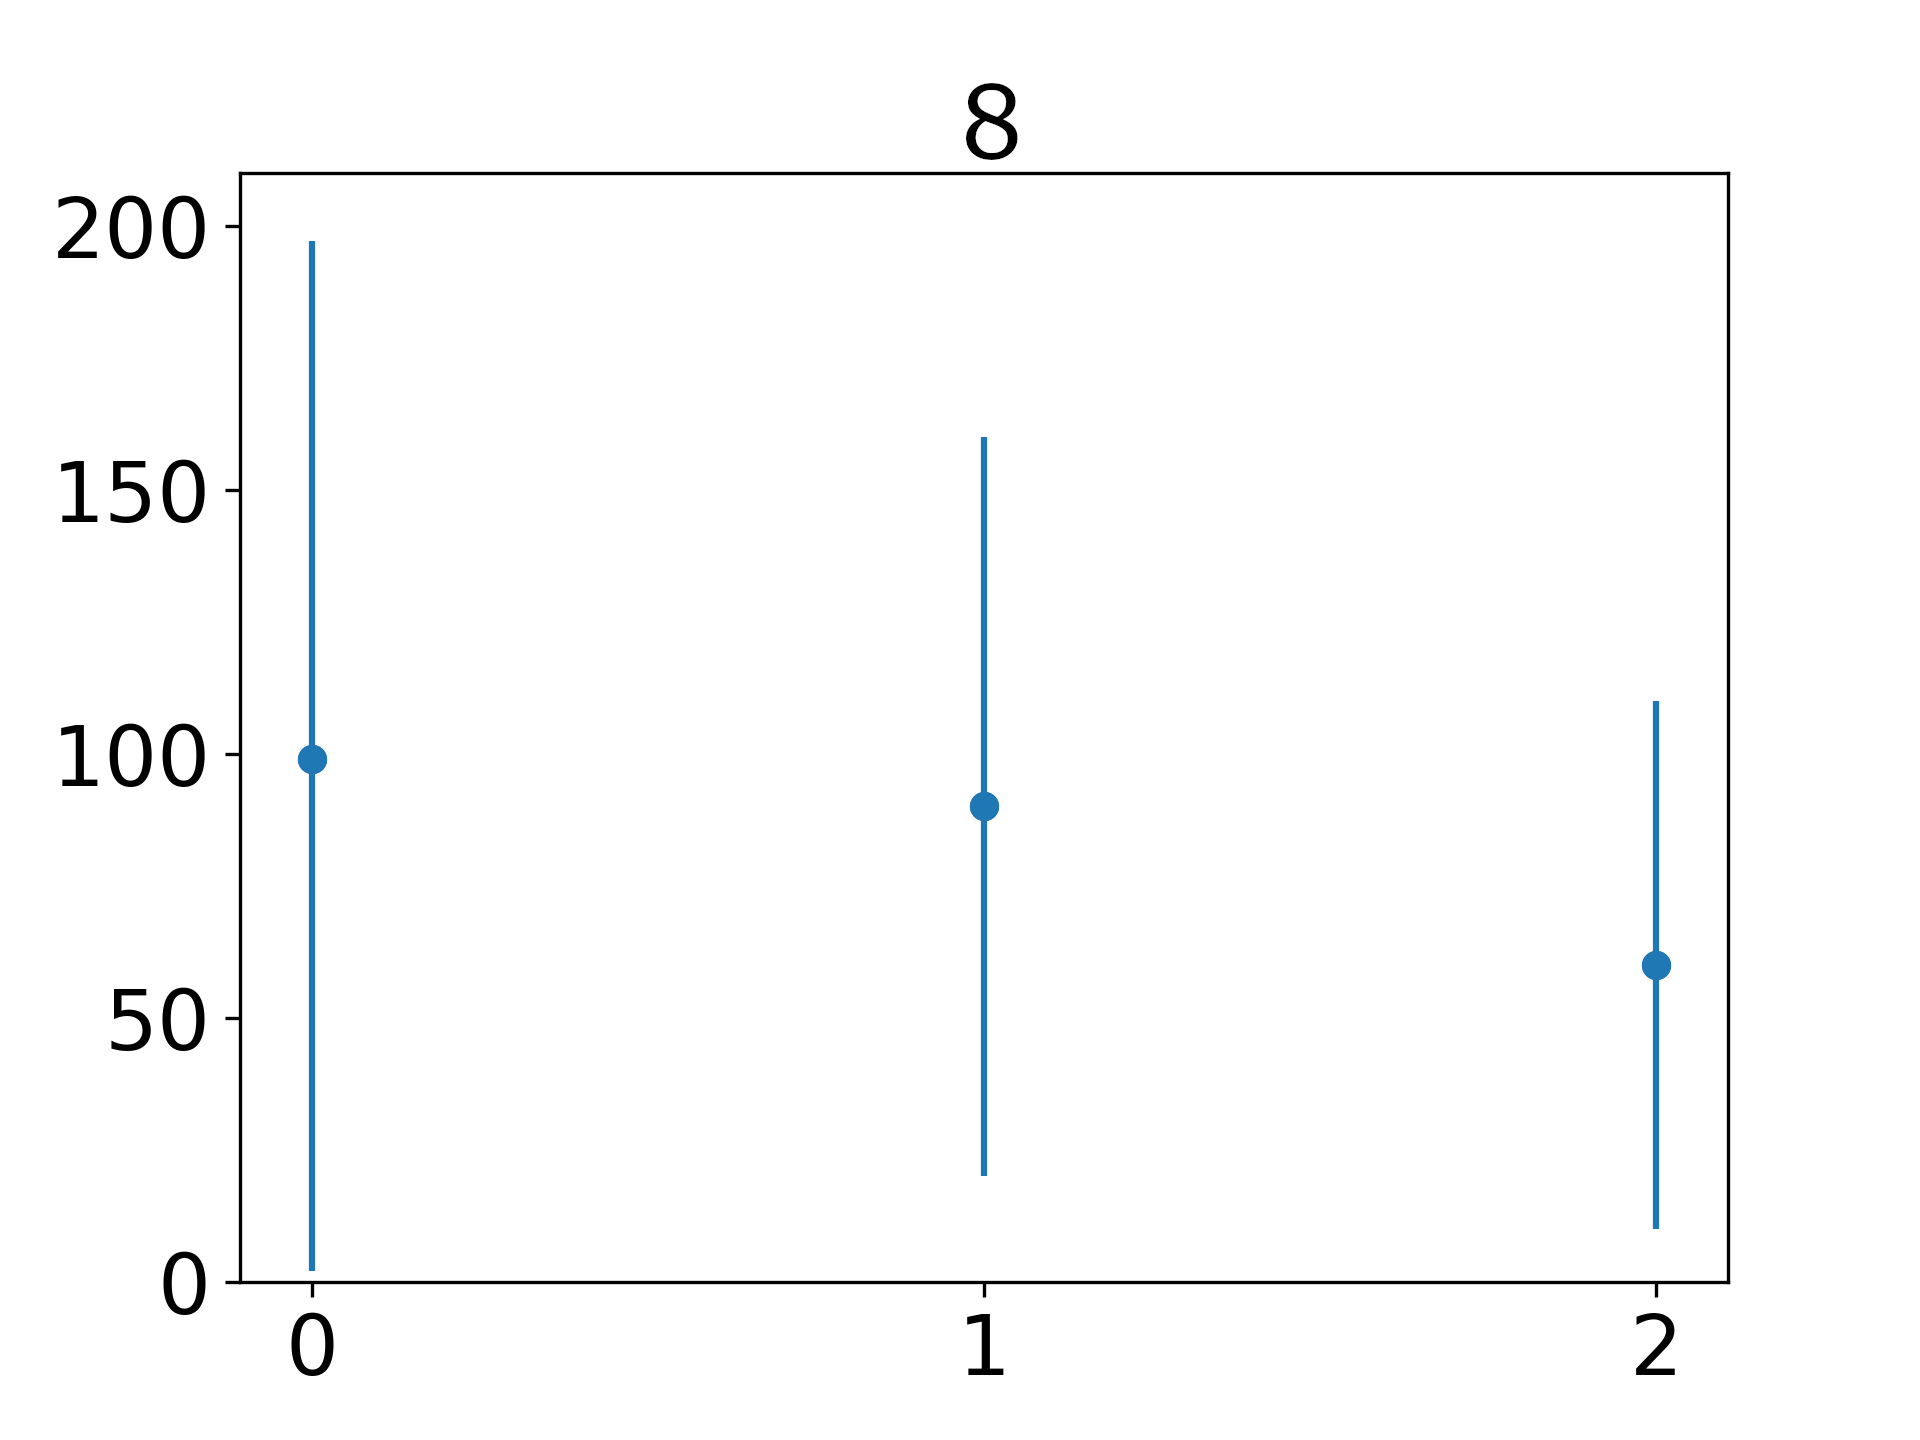
\includegraphics[scale=0.27]{Images/Average_steps/h.png}
\end{subfigure}
\caption{Average number of steps for the agent to reach the goal when trained with rewards generated from brainwaves from OHCs 1-8. Y axis show the averaged number of steps for a run session, while x axis show the number of game matches used to cumulative train the Q-Table.}
\label{fig:avg_steps}
\end{figure}


The results show that as the Q-Table is progressively trained the average amount of steps decreases, meaning that the agent learns. However, the rate at which it learns varies per OHC, depending on the classification accuracy of the extracted brainwaves.  For example results for OHC 1 show faster learning than those of OHC 8 (Figure \ref{fig:avg_steps}).

In the case for OHC 5 and 6, the reward information obtained from the brainwaves is not enough to train the agent effectively. Figures \ref{fig:avg_steps} for OHC 5 and 6 show no apparent learning, as the amount of steps to reach the goal doesn't decrease when trained.  These results are also consistent with their classification ROC curves, shown in Figures~\ref{fig:rocsubjects} obtained for both OHCs, where the area under the curve are close to chance level.  Both OHCs have less recorded data from the sessions in comparison to the rest of the OHCs.  This variation in performance for different OHCs has been studied extensively in BCI~\cite{Chavarriaga2014}.  Besides low data samples, there are other reasons affecting the classification accuracy:  cognitive reasons (i.e. the OHC not paying extensively attention to the game dynamics), very low SNR of the ErrP component or even the BCI-illiteracy phenomena where the specific OHC's signals do not contain the expected component response~\cite{Yousefi2019}.

\begin{figure}[h!]
\captionsetup[subfigure]{justification=centering}
\begin{subfigure}{0.5\textwidth}
\centering
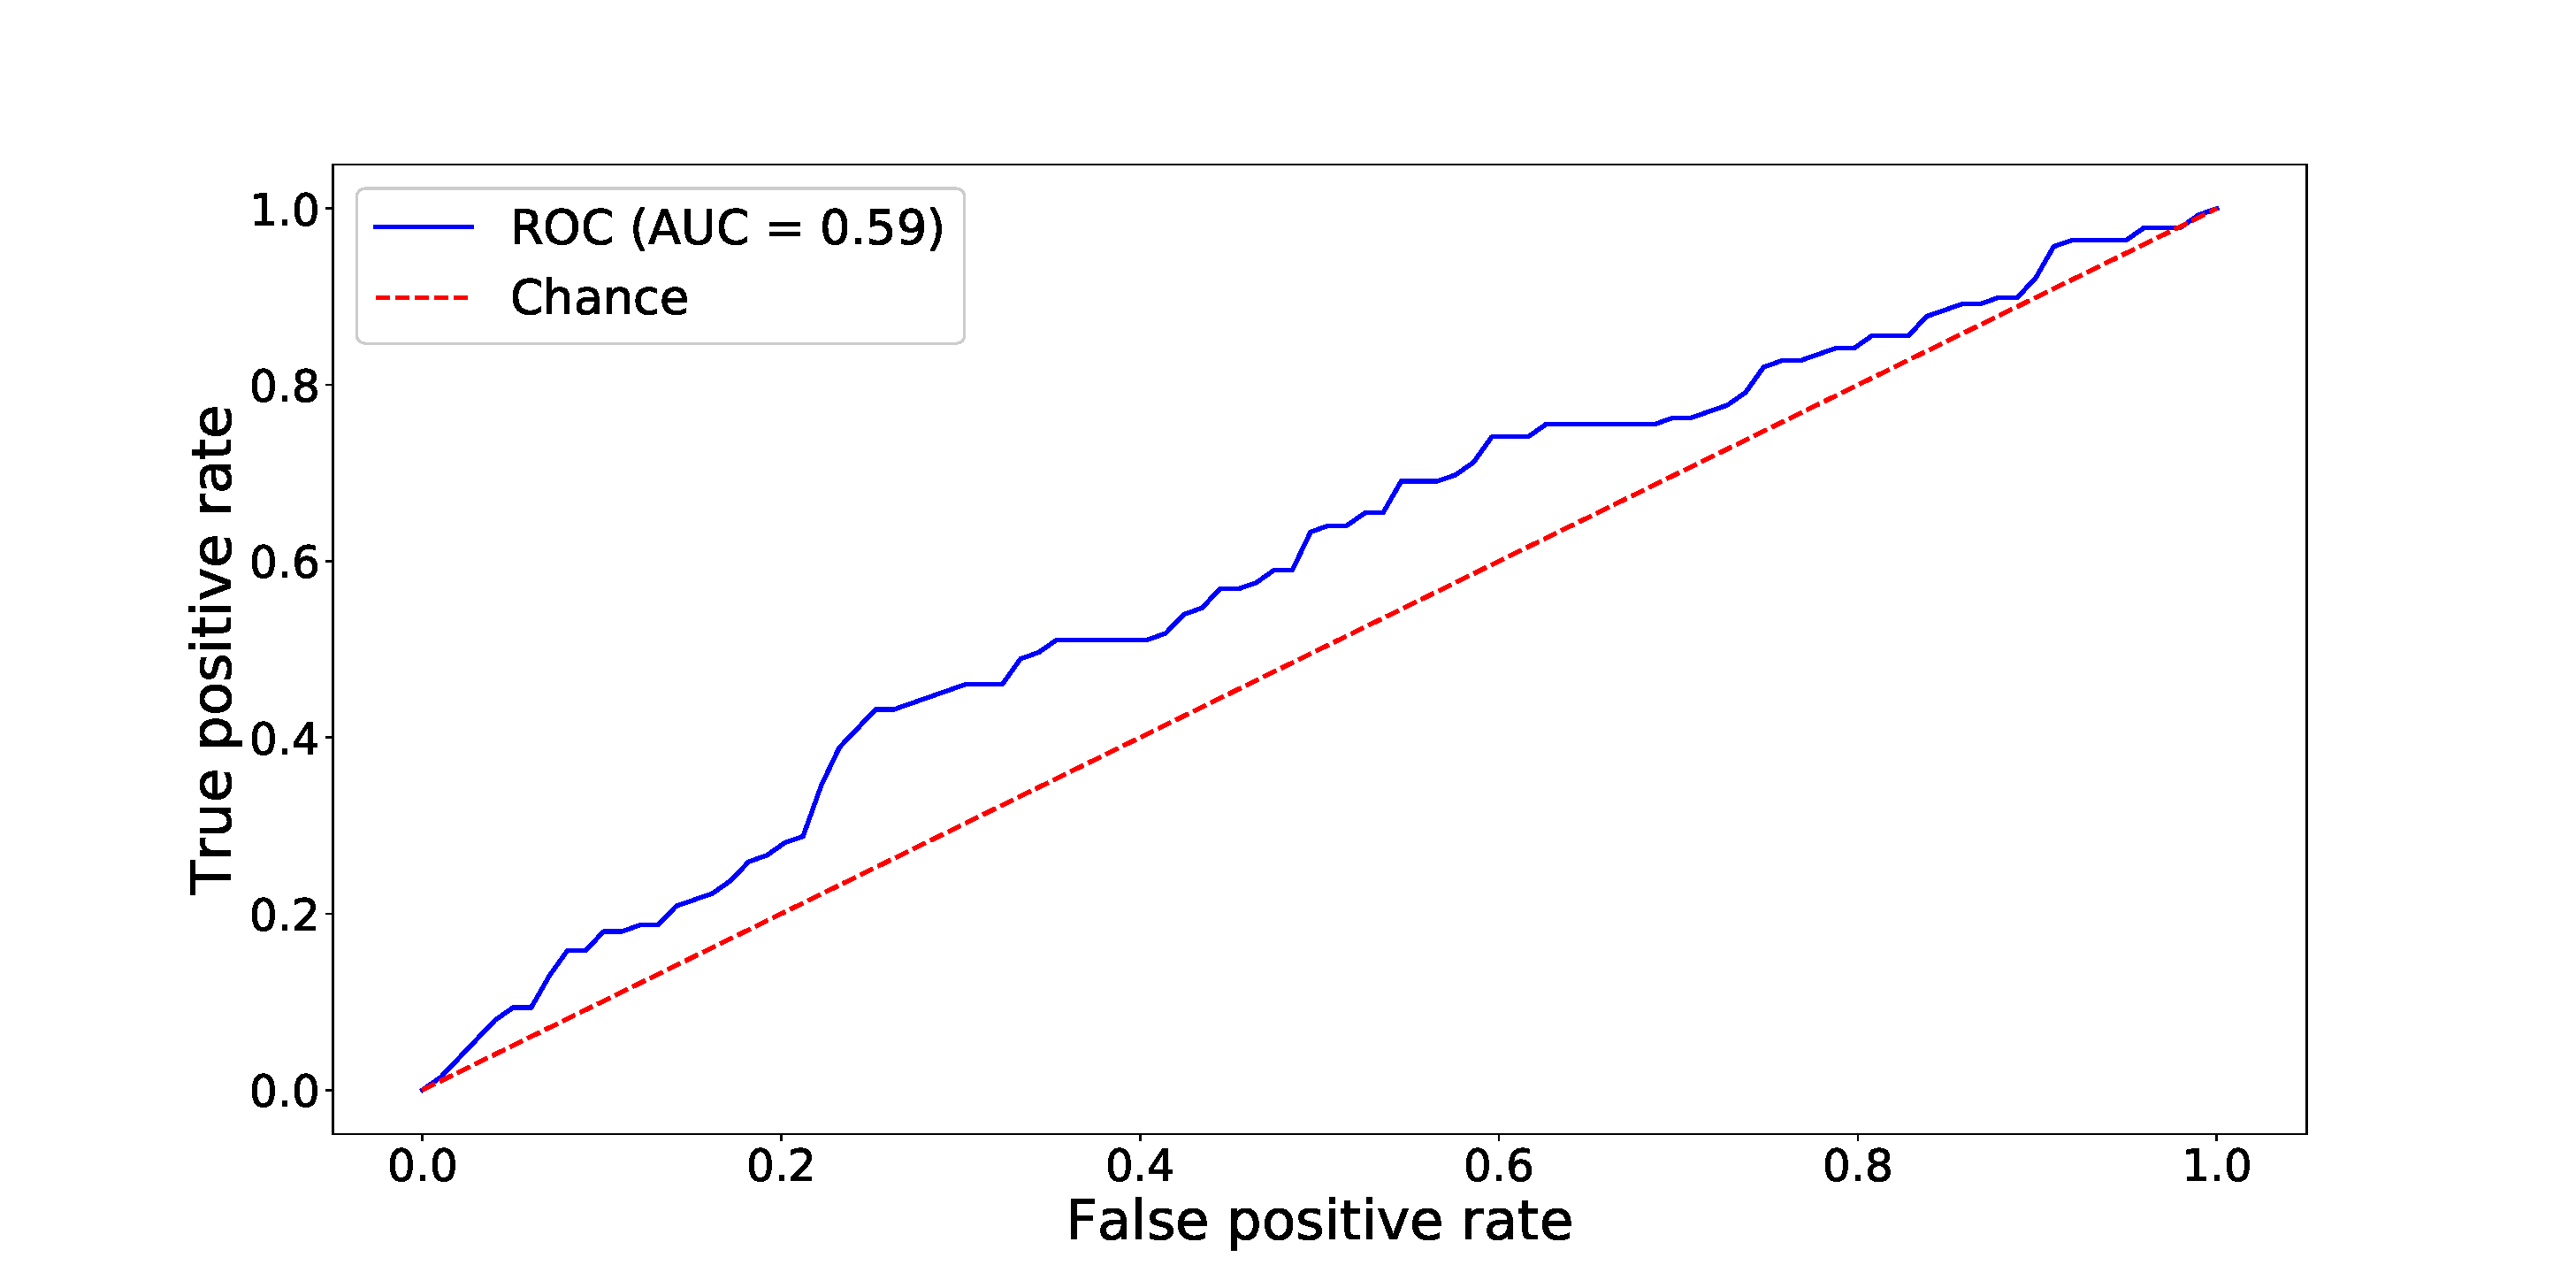
\includegraphics[scale=0.09]{revisedimages/roc_1.eps}   \hspace{-1.5em}
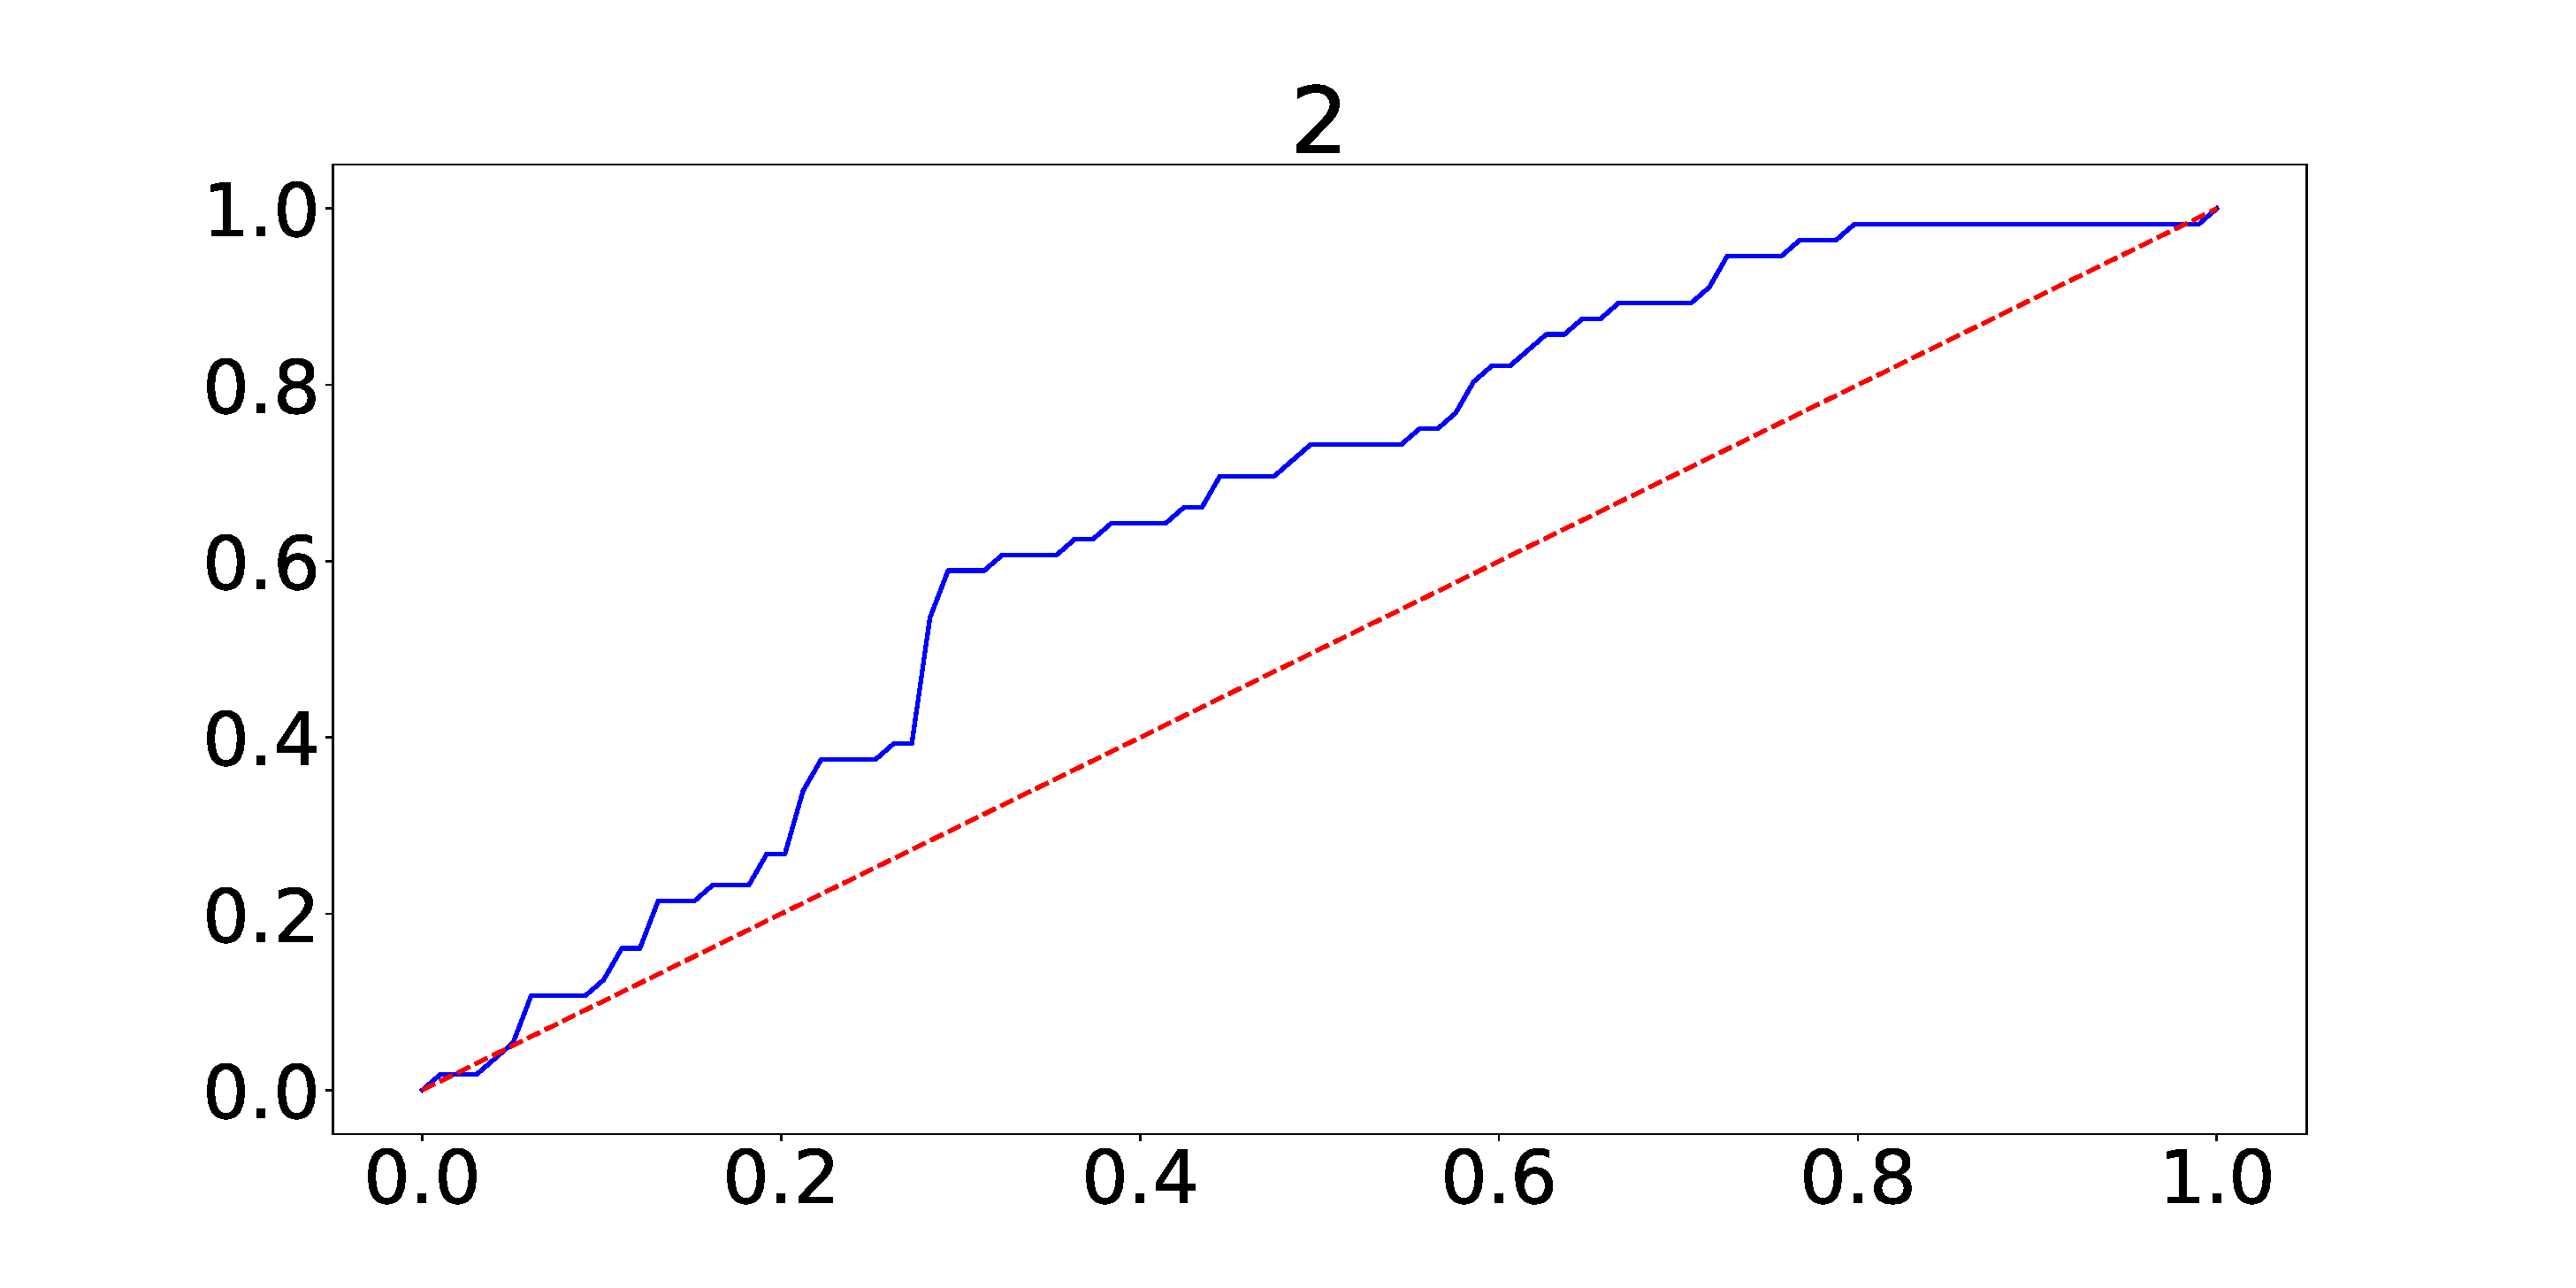
\includegraphics[scale=0.09]{revisedimages/roc_2.eps} \\
%\vspace{-1.3em}
\centering
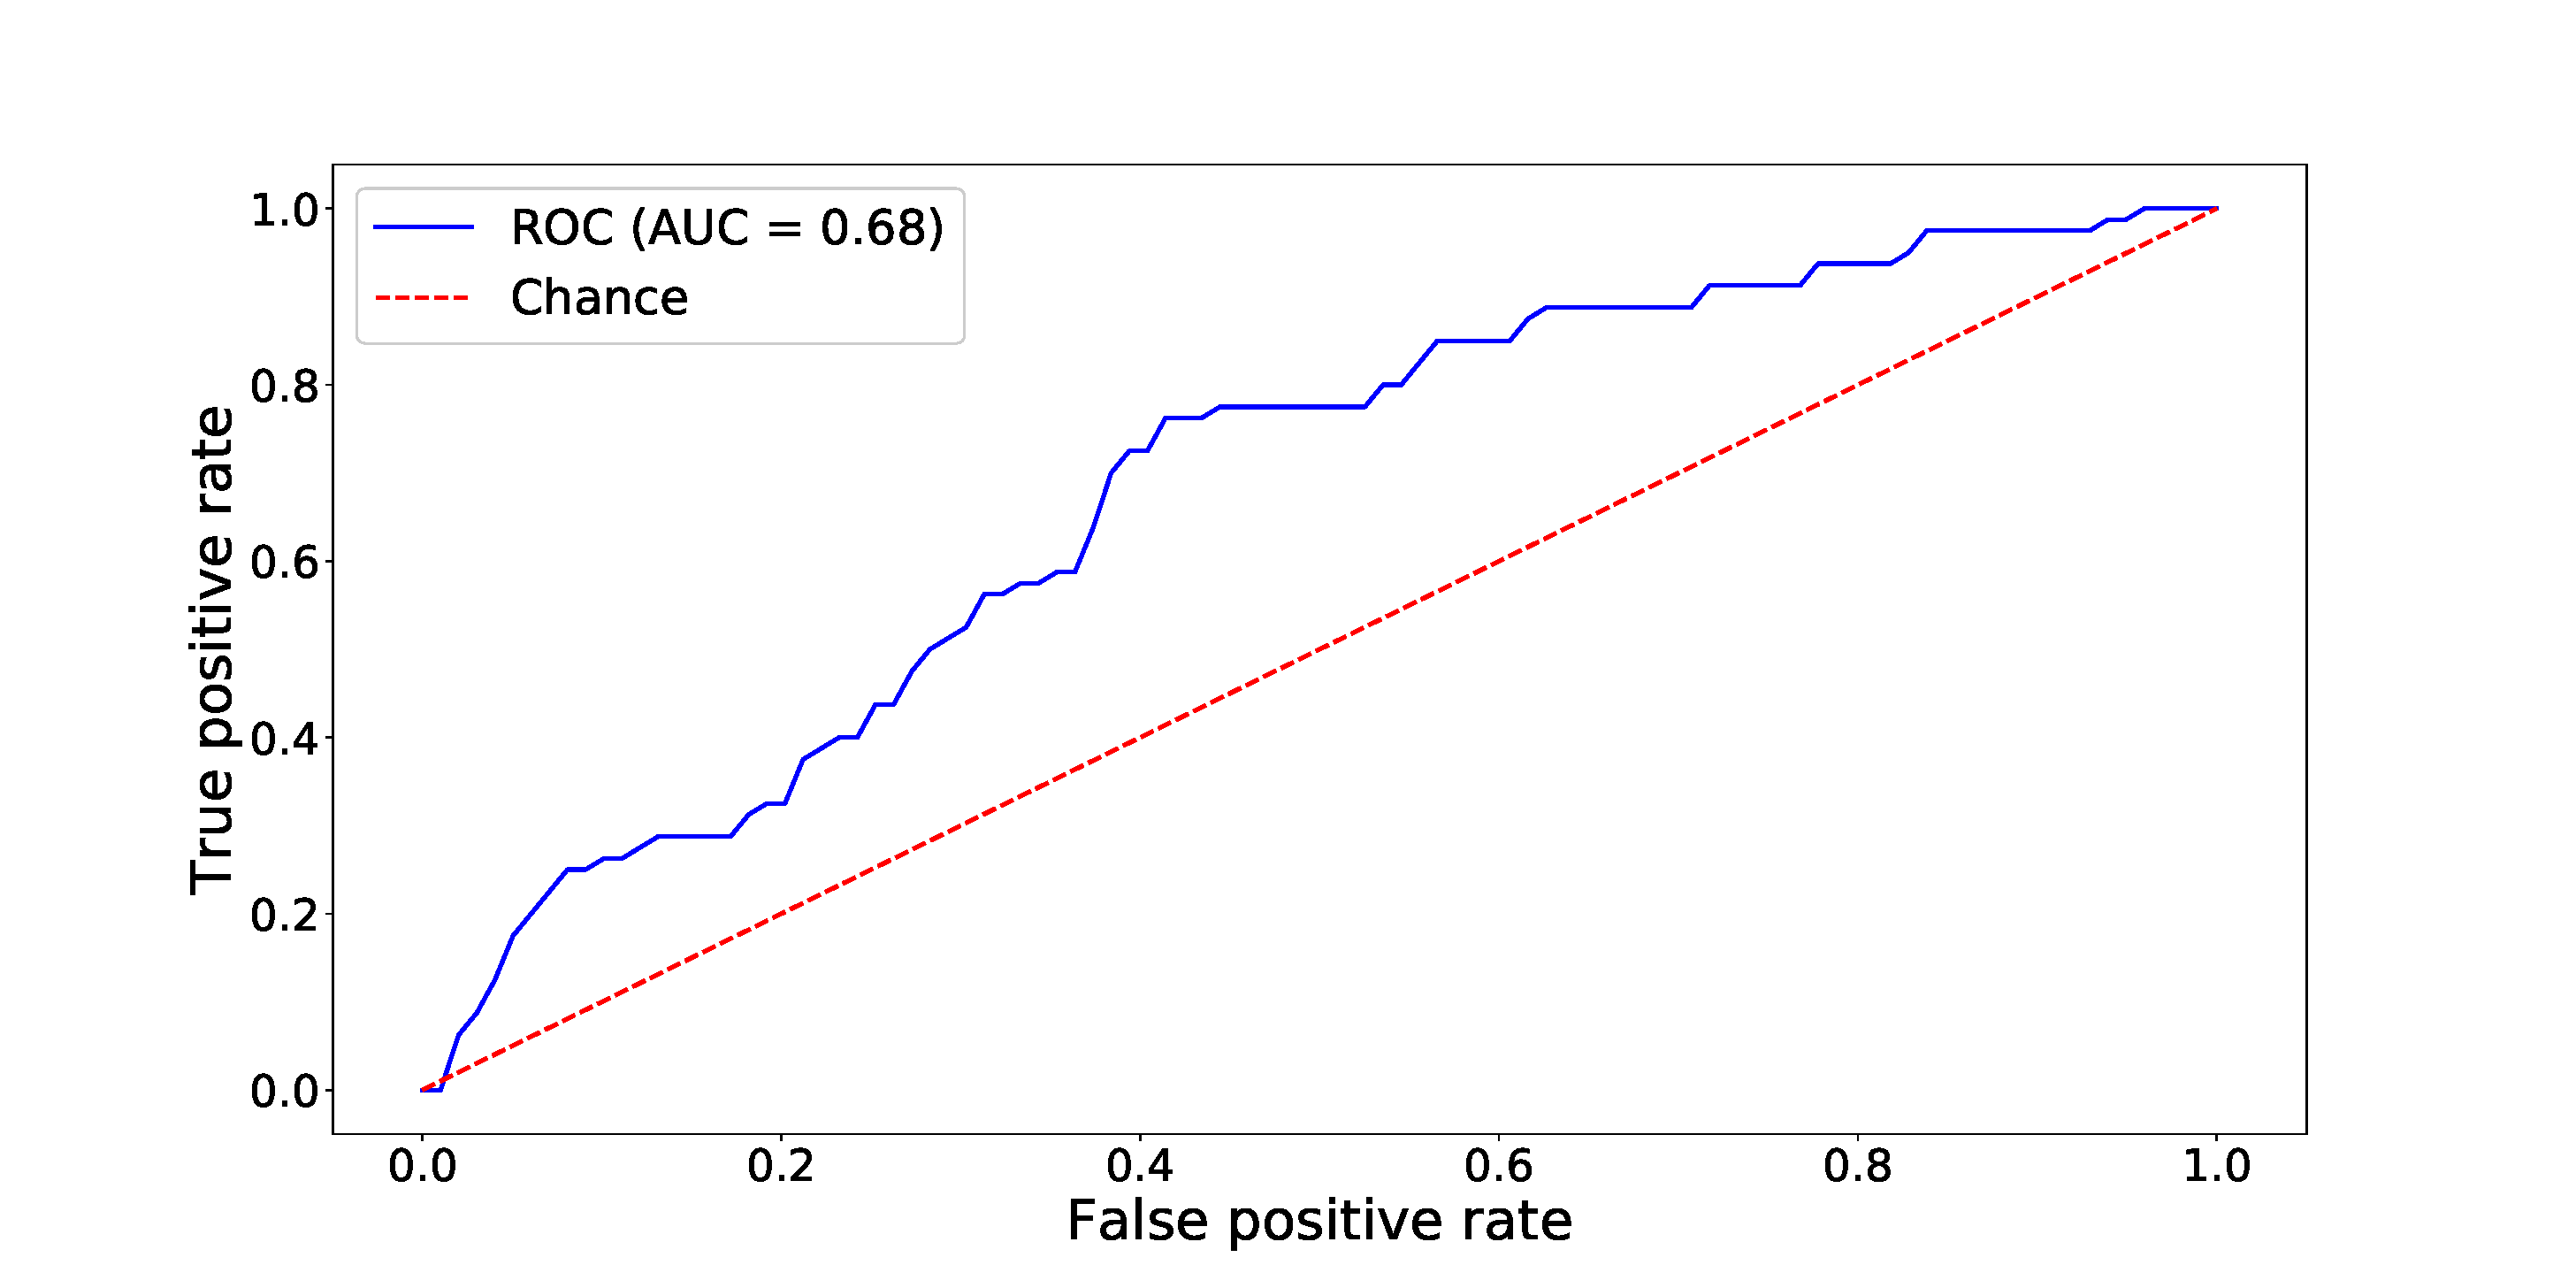
\includegraphics[scale=0.09]{revisedimages/roc_3.eps}   \hspace{-1.5em}
 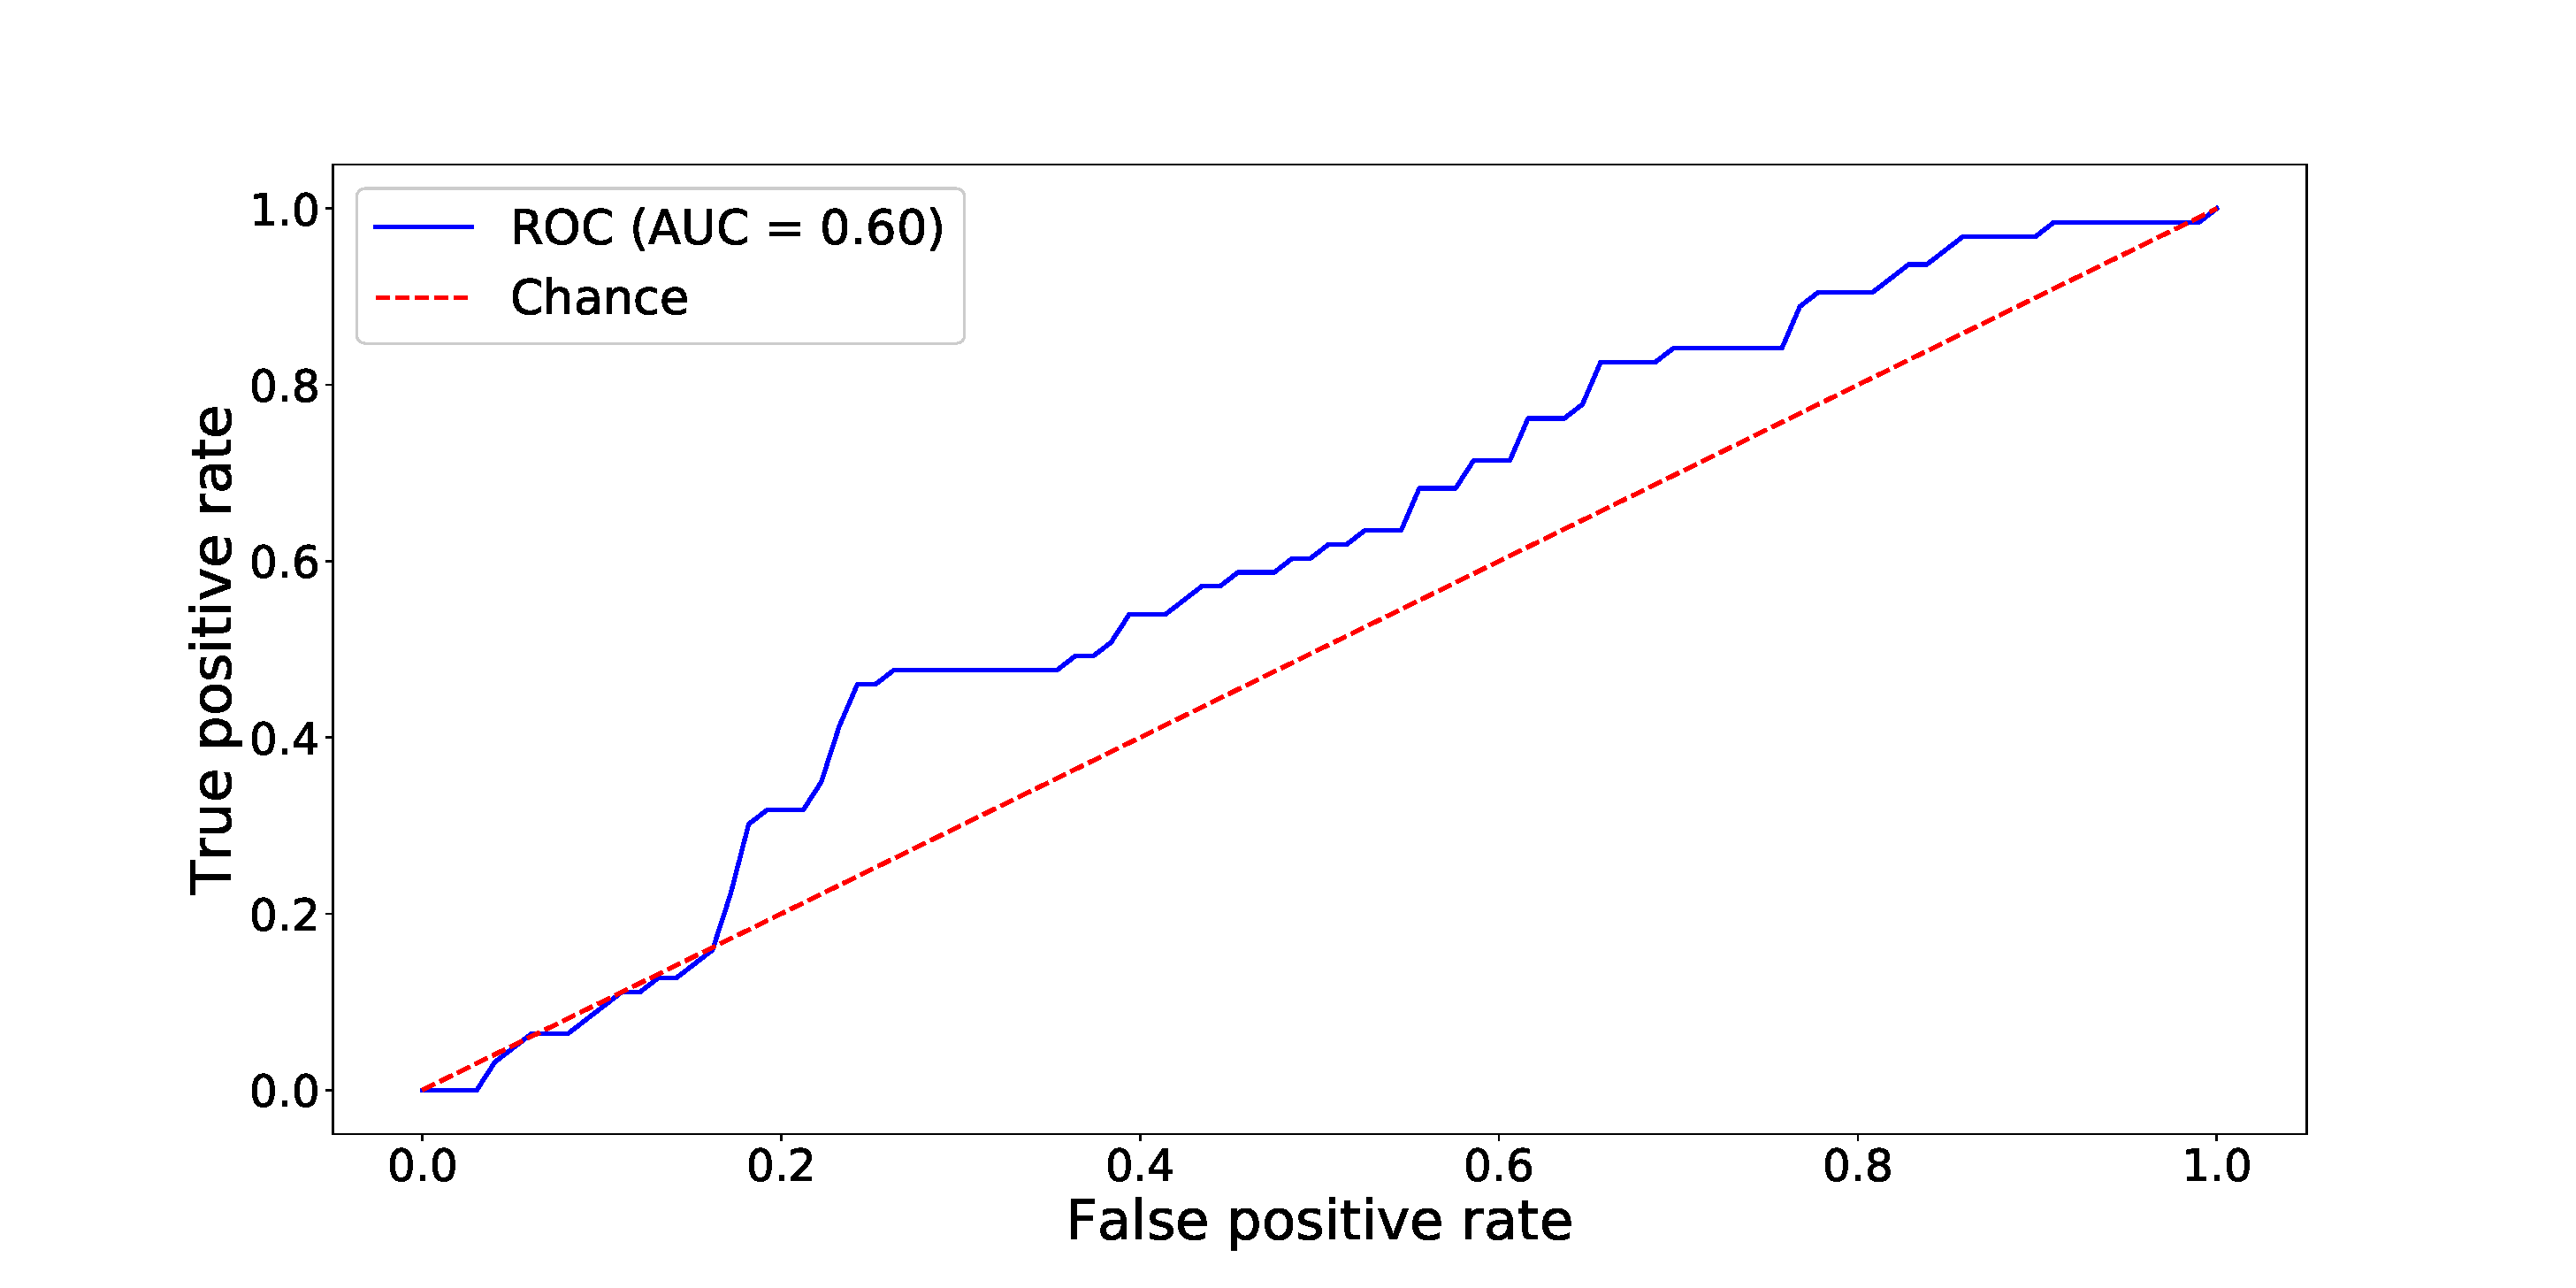
\includegraphics[scale=0.09]{revisedimages/roc_4.eps} \\
 \centering
  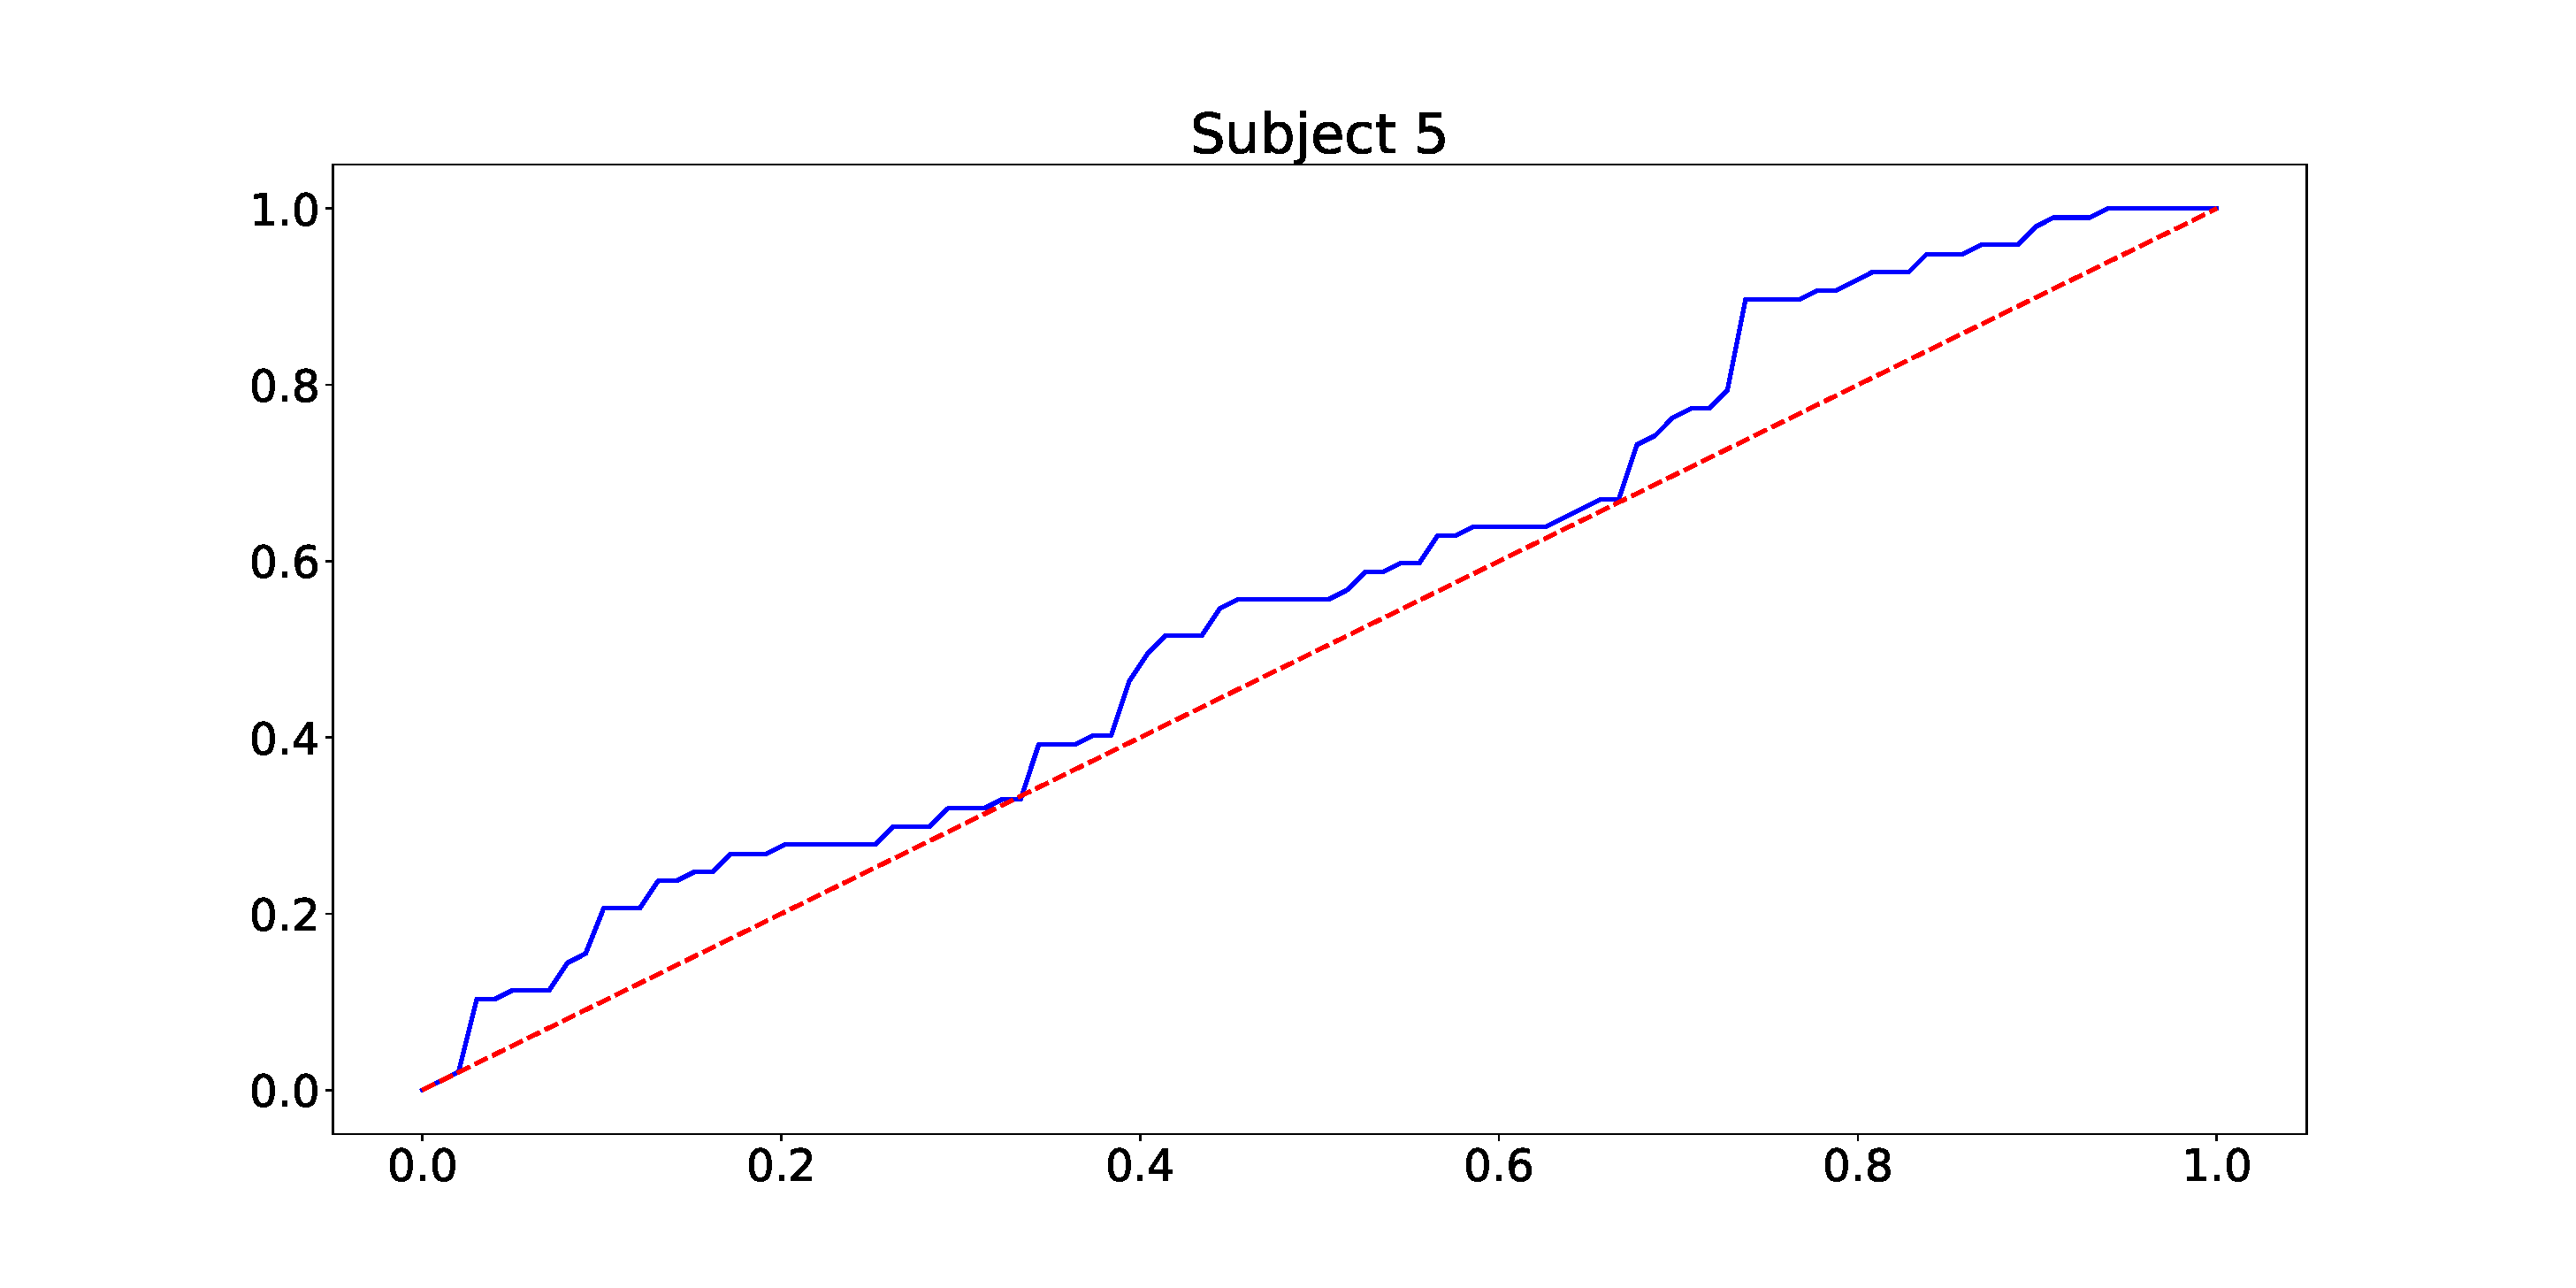
\includegraphics[scale=0.09]{revisedimages/roc_5.eps}   \hspace{-1.5em}
  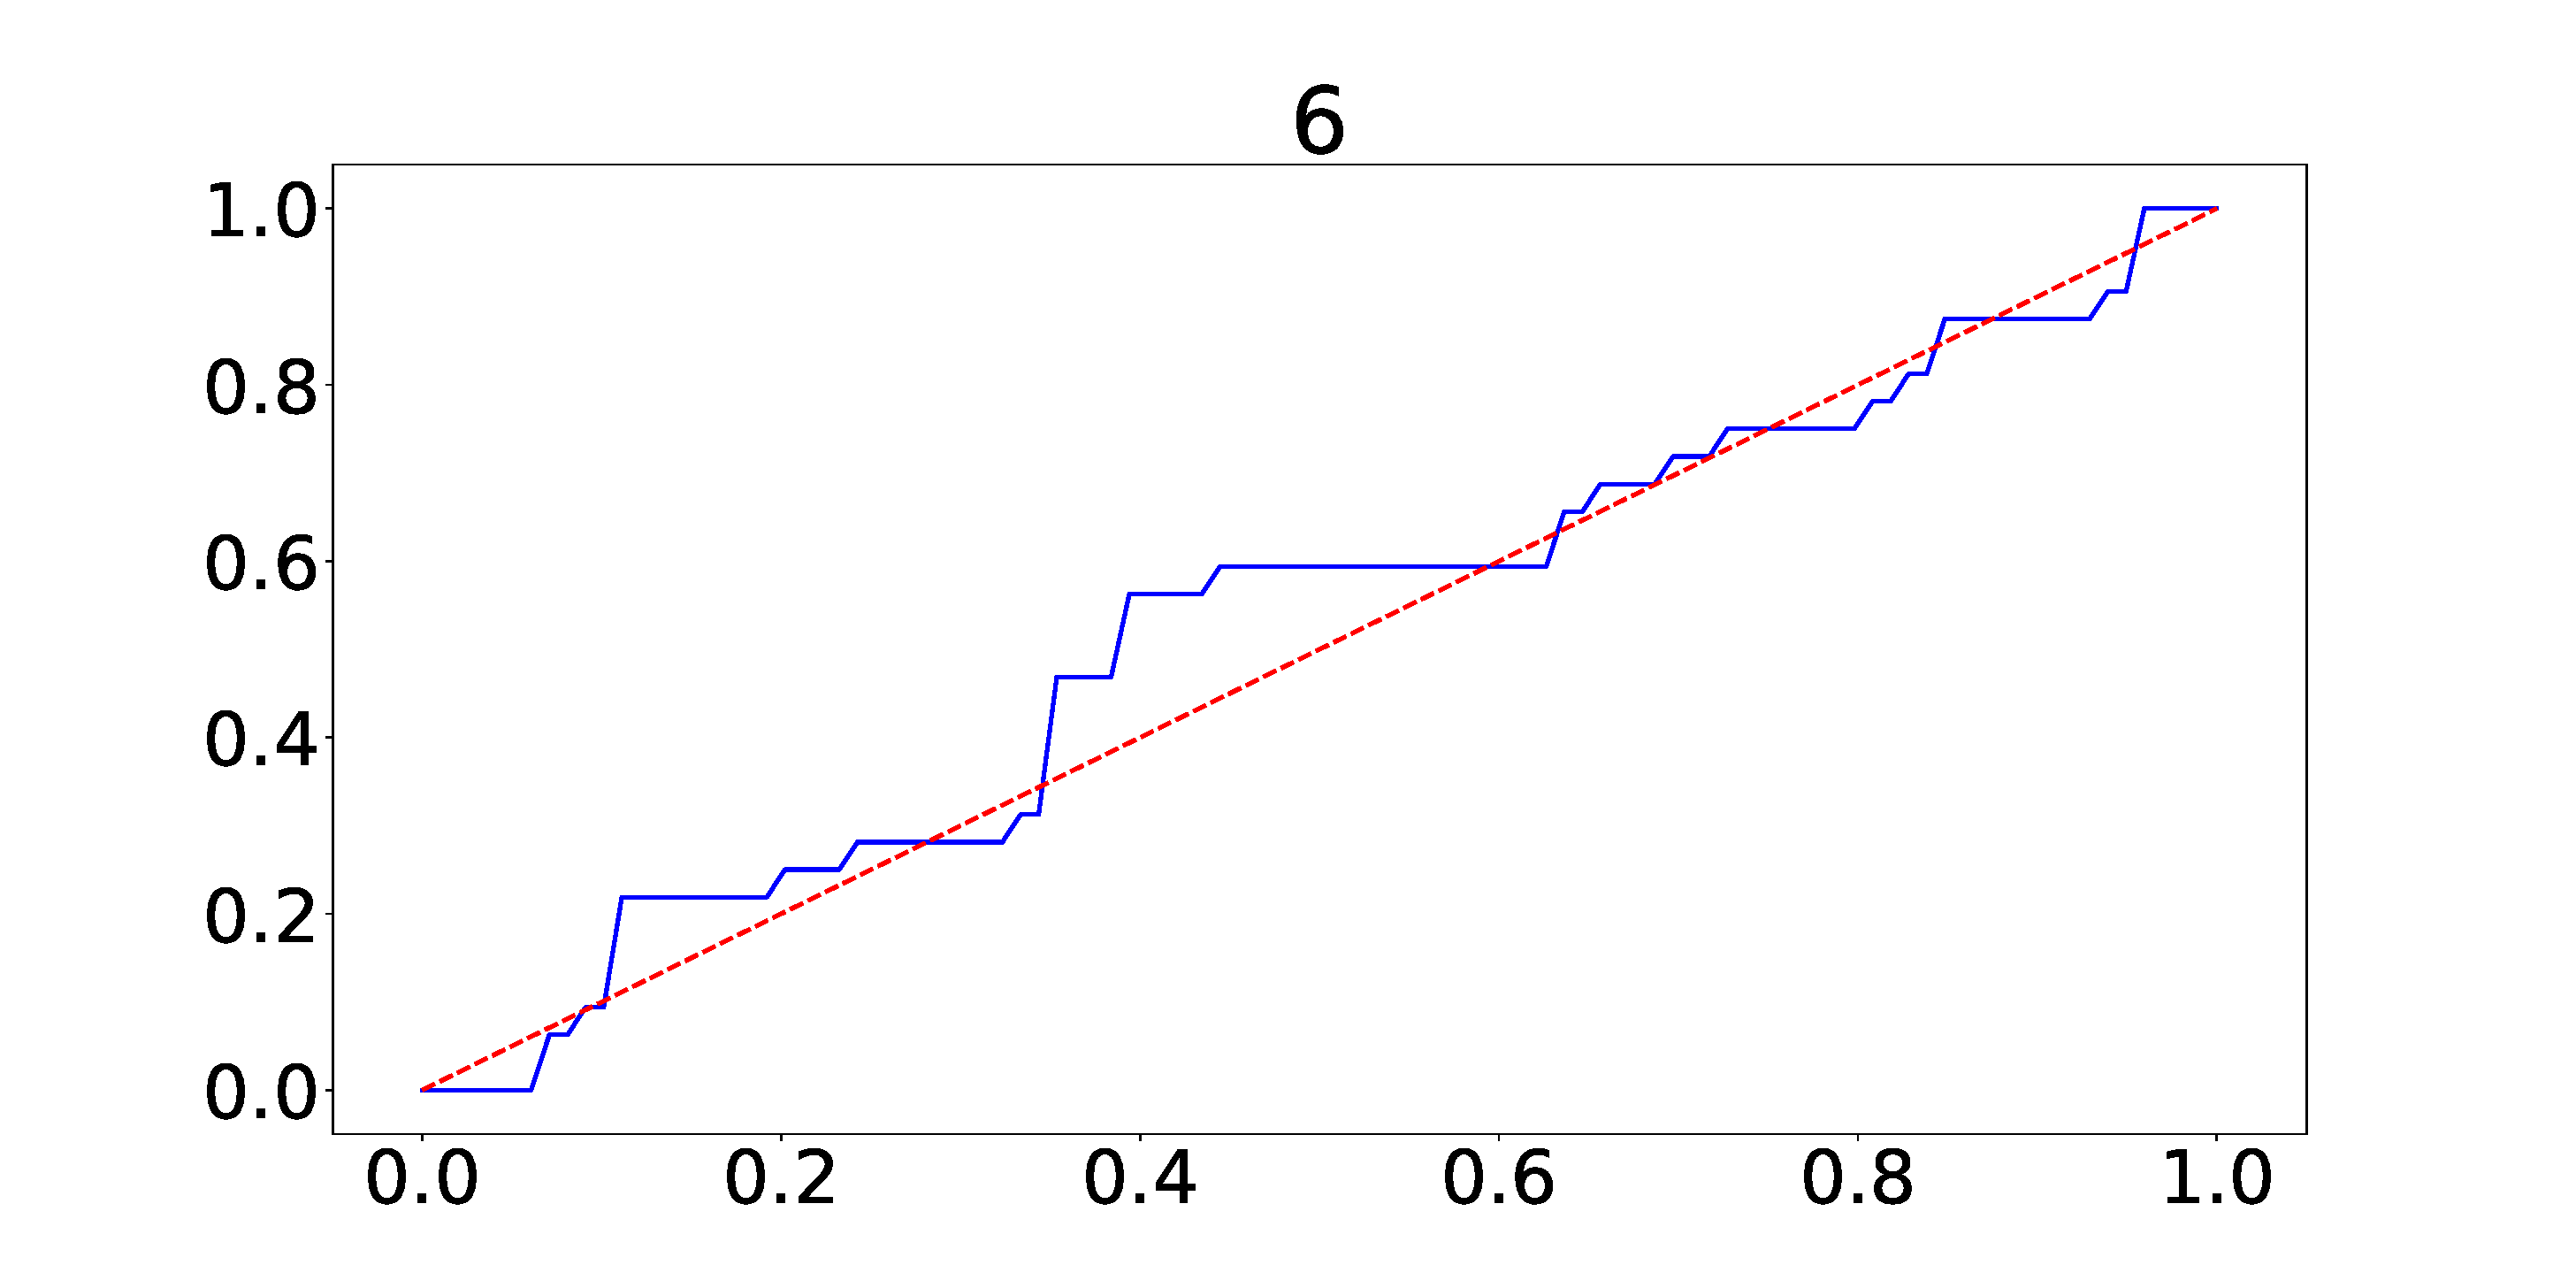
\includegraphics[scale=0.09]{revisedimages/roc_6.eps} \\
  \centering
  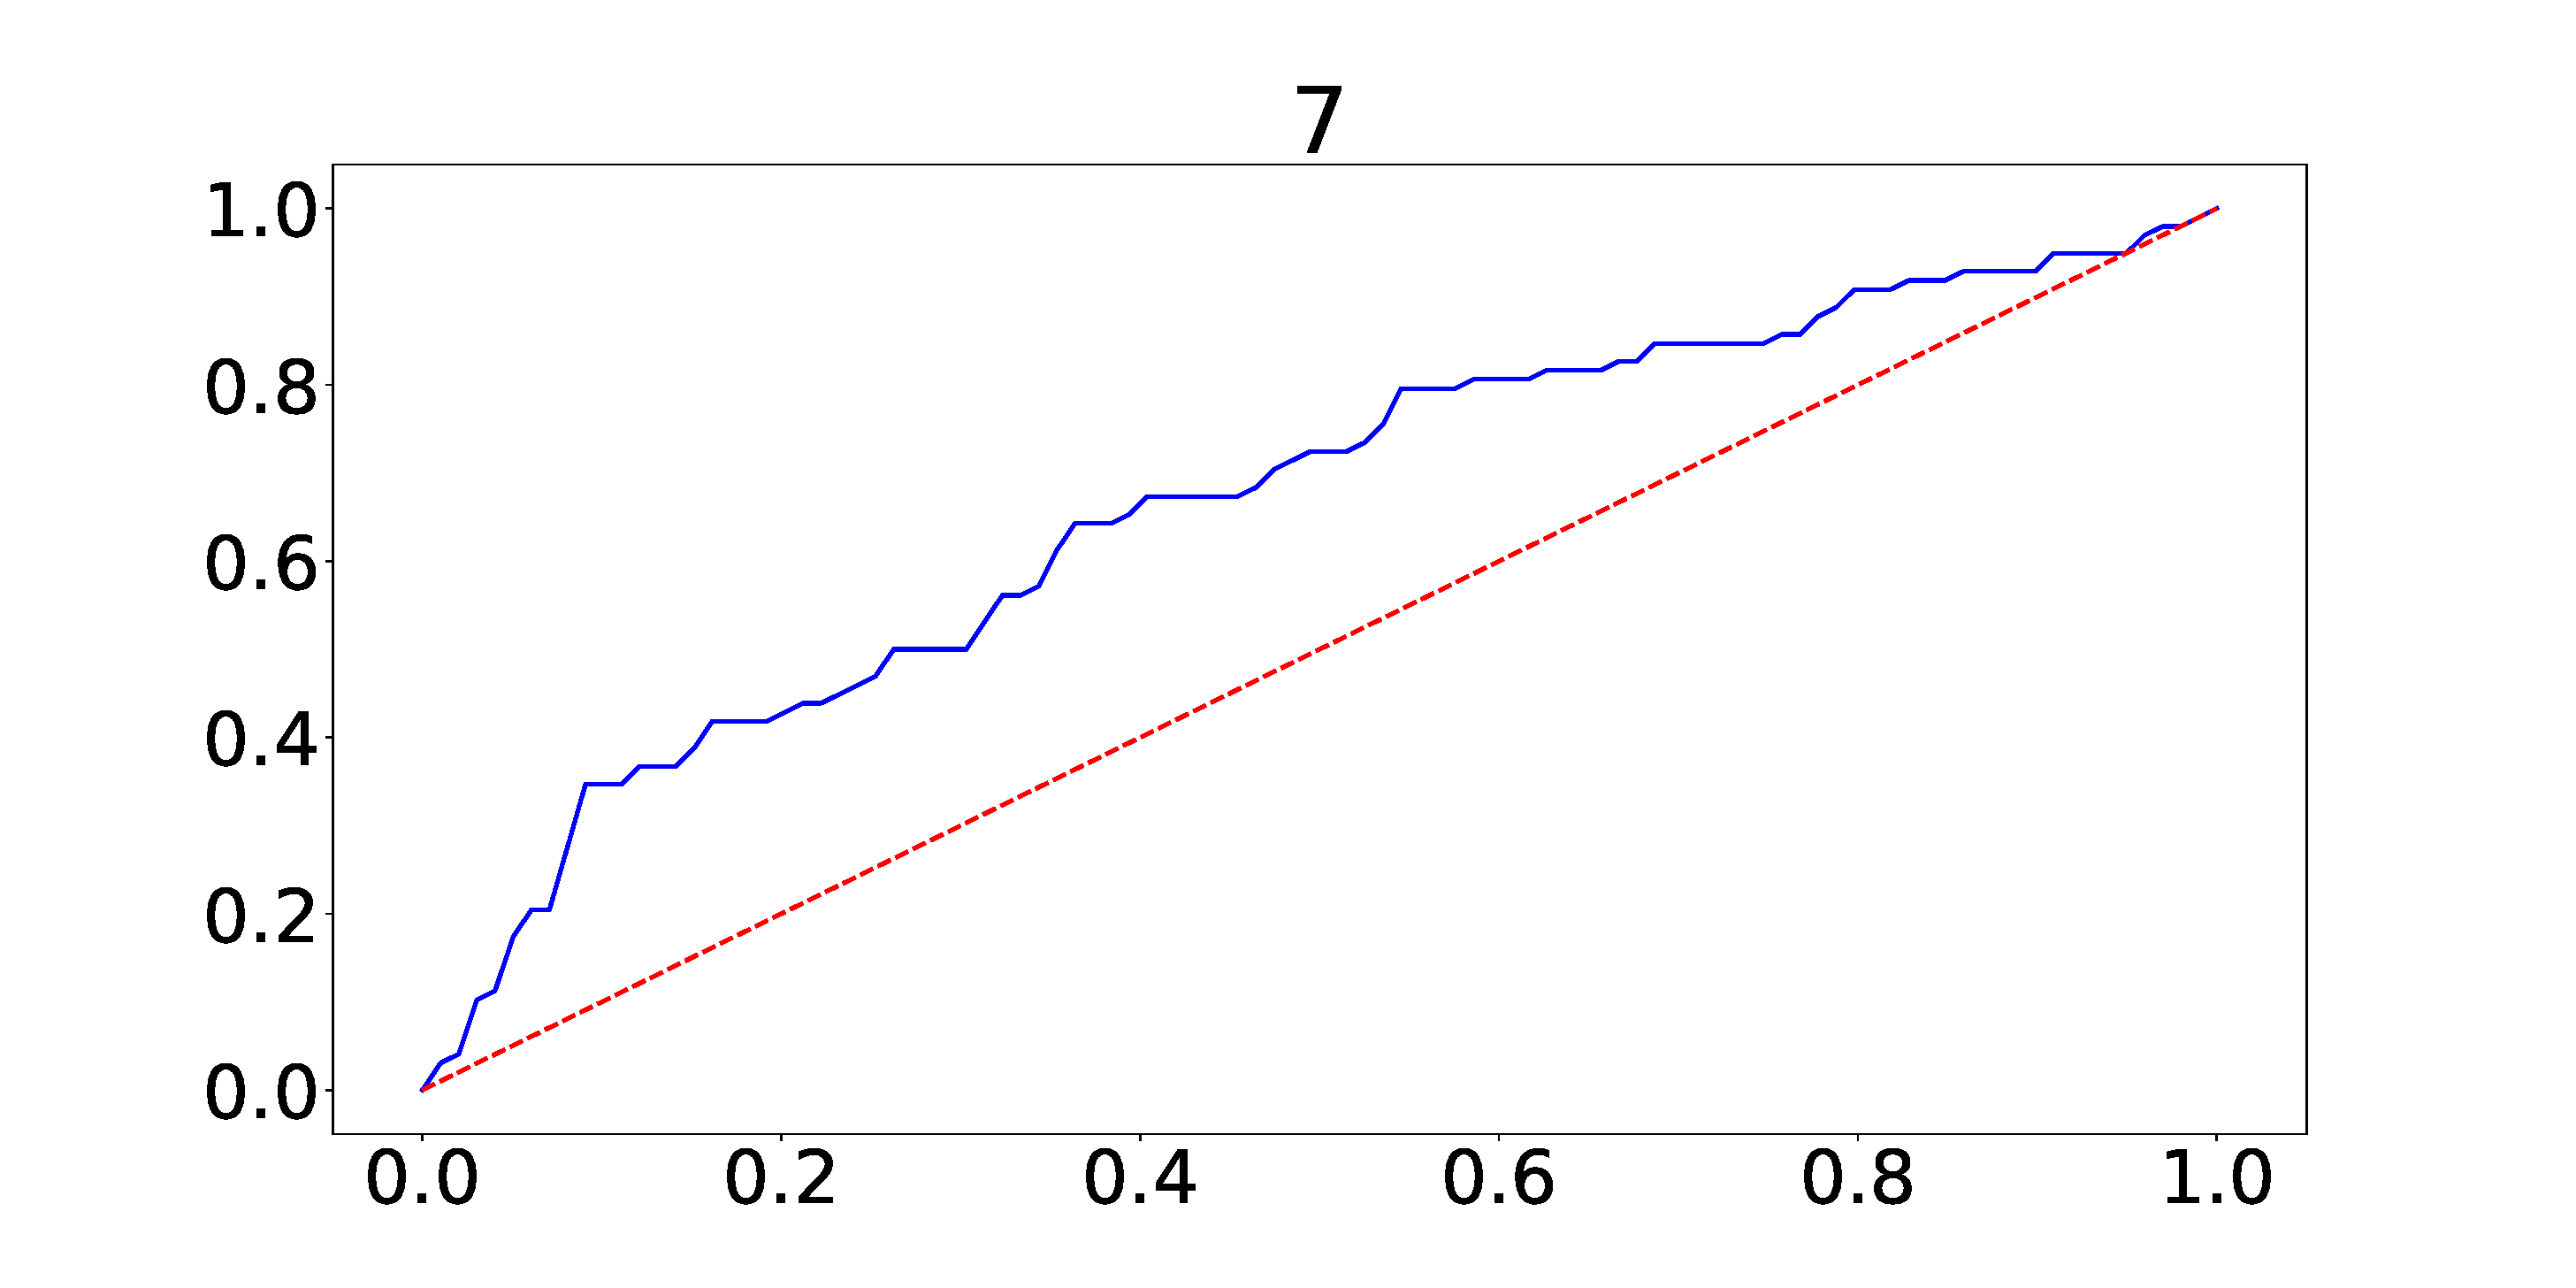
\includegraphics[scale=0.09]{revisedimages/roc_7.eps}    \hspace{-1.5em}
  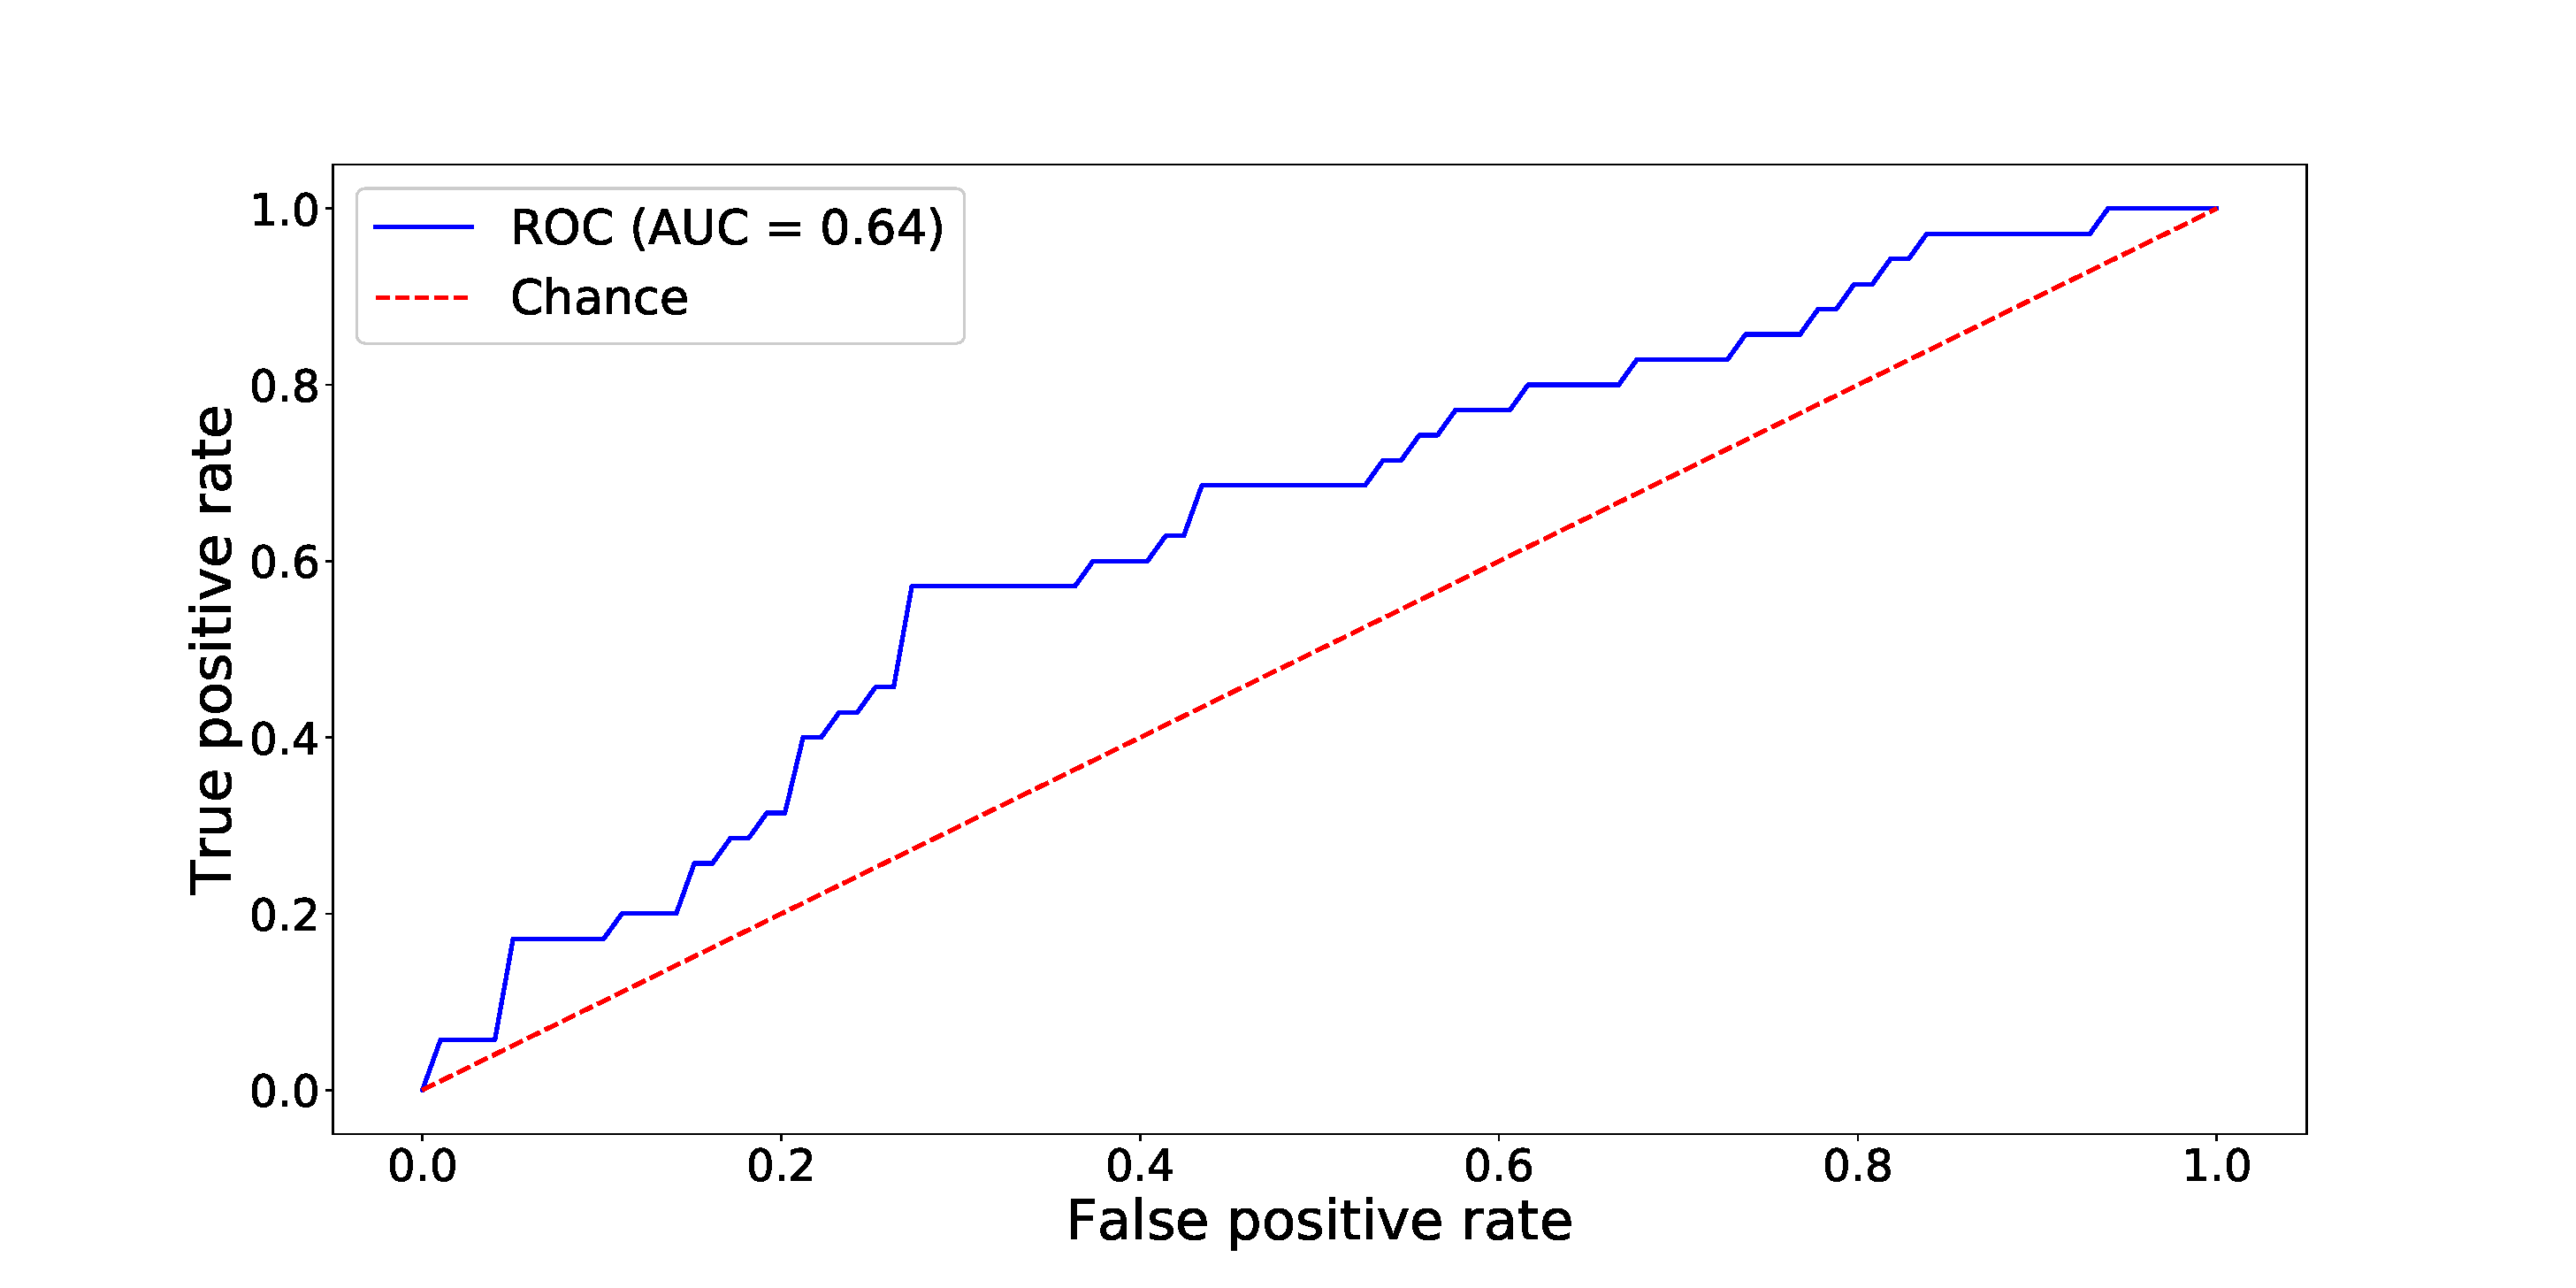
\includegraphics[scale=0.09]{revisedimages/roc_8.eps} \\
\end{subfigure}
\caption{ROC Curves for OHCs 1-8. True positive rate is on the vertical axis and false positive rate on the horizontal axis.}
\label{fig:rocsubjects}
\end{figure}

%These results are consistent with fig. \ref{fig:roc:e} and fig. \ref{fig:roc:f}, which show that the signal classification for these subjects hasn't been particularly successful.

Figure~\ref{fig:avg_steps_noise} shows the result of an agent successively trained with brainwave session matches where the EEG is generated with random signals.  In this case, random EEG signals are generated using OpenVibe Acquisition Server signal generator for all channels, as if they were produced by an OHC who doesn't pay attention to the game.  The agent learns nothing, and regardless of the number of matches that are used to learn the Q-Table, the number of steps required to reach the goal does not decrease.  This pattern is also obtained when the game matches from OHCs 5 and 6 are used, showing that the reward labeling predicted by the trained classifier for those cases worked like a random classifier.

\begin{figure}[h!]
\centering
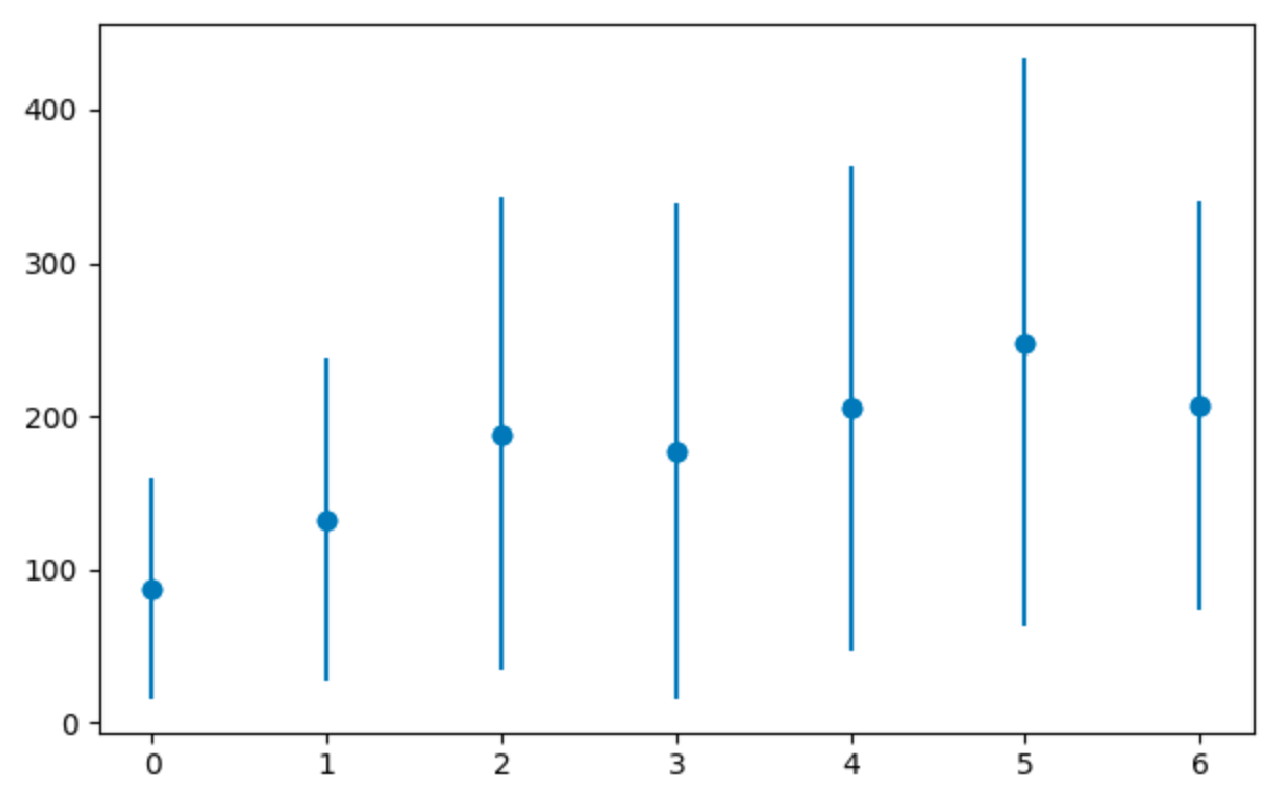
\includegraphics[scale=0.4]{Images/Average_steps/noise.eps}
\caption{Average number of steps for the agent to reach the goal when trained with a classifier produced from sham EEG signals. X axis show the number of gaming agent training matches used to train the Q-Table.}
\label{fig:avg_steps_noise}
\end{figure}

Electroencephalographic signals have high inter-subject variability~\cite{Chavarriaga2014}.  This is evidenced in Figure~\ref{fig:transferlearning} where the agent training is performed with rewards obtained by classifying epochs from one Tester OHC and a classifier that was trained using the brainwaves from a different Trainer OHC.  The figure shows the cumulative variation for all run sessions on the average number of steps required to reach the goal after training the agent with all the available matches from the brainwave session.  Enhancements are shown as negative values.  Only the diagonal of the heatmap matrix shows a clear improvement in terms of the reduction of the required number of steps to reach the goal (averaged per 200 runs) which corresponds to the same information for each OHC shown in Figure~\ref{fig:avg_steps}.  For the transfer learning experiment~\cite{Wu2016}, no performance gain is evidenced, the agents learn nothing and this implies that the reward information provides no value.


\begin{figure}[h!]
\begin{subfigure}{0.5\textwidth}
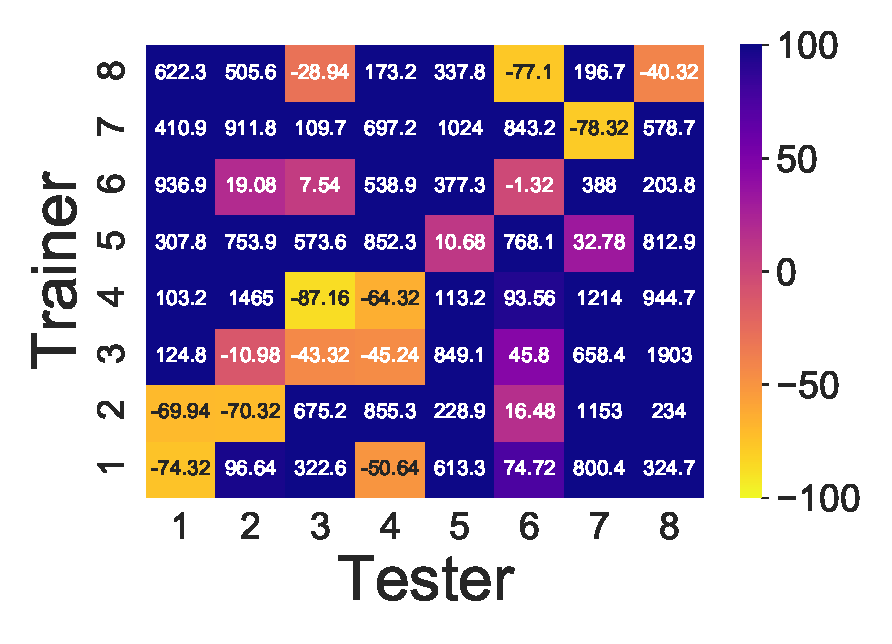
\includegraphics[scale=0.60]{revisedimages/transfer_learning_heatmap.eps}
\end{subfigure}
\caption{Heatmap for the transfer learning experiment. Values represent the reduction in the average number of steps required to reach the goal.  Negative values represent net improvements.}
\label{fig:transferlearning}
\end{figure}

Finally, Figure~\ref{fig:avg_steps_all} shows the result of training an agent with cumulative brainwave session matches from OHCs 1, 2, 3, 4, 7, and 8.  It can be seen that the overall performance of the agent improves as long as there is information to produce rewards, regardless of the fact that they were generated from classifiers trained with different OHC's signals.


\begin{figure}[h!]
\centering
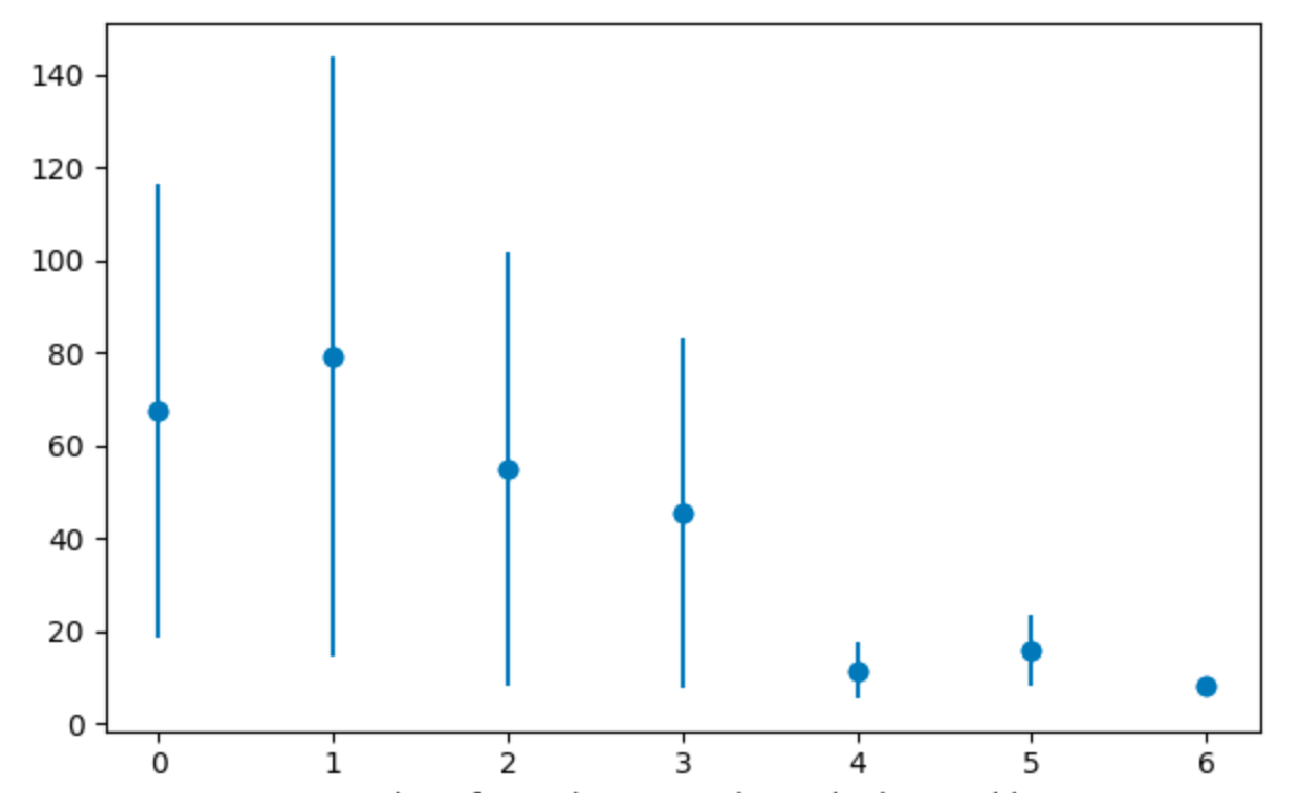
\includegraphics[scale=0.4]{Images/Average_steps/all.eps}
\caption{Average steps using Q-Table trained with brainwave session matches from six different OHCs. X axis show the progressive number of gaming agent training matches used to train the Q-Table. These matches correspond to all subjects, excluding subjects 5 and 6 which individually show no significant learning progress.}
\label{fig:avg_steps_all}
\end{figure}

\section{Conclusion}
\label{conclusions}

%Enfatizar la idea de que la mejor métrica de la propia detección está dada por la propia capacidad del agente de minimizar su tarea, que hay un flujo de información que involucra la propia percepción de la persona.

This work aims to propose a simple game mechanics that can use the ErrP component to train a gaming agent using a RL model. The collected data and the shows that ErrP signals can in fact be classified and used to train an agent effectively.

This proposal tries to keep the system as simple as possible, emphasizing information flow from the subjective error perception of the human critic. Rewards are generated using the signal processing and classification pipeline, and the Q-Table updates, enhancing the performance of the gaming agent.

One additional aspect to remark is the robustness of the learning strategy based on Q-Learning~\cite{Bauer2015,Rubin2012}.   The obtained accuracy to discriminate ErrPs is low, though on the same level to other similar results~\cite{Iturrate2013,Ehrlich2016}.  In this regard, dispite of the subjectivity of the ErrP response in terms of the proposed experiment, levels of 90\% of accuracy are reported~\cite{Chavarriaga2014}.  However, even with such low accuracy values, the RL algorithm was able to extract meaningful information from rewards that were helpful to improve, and often maximize, the agent's performance.  Additionally, one important aspect of the classification results is the low percentage of false positives (Figure~\ref{fig:confusionmatrix}), showing a high specificity. On the other hand, the percentage of false negatives is generally higher.  However, even though this implies that the agent misses frequently when a wrong action takes place, this is not hindering the overall performance and the agent is still learning. Though scarce, accurate rewards are very useful for the RL algorithm.
%However, even though this imply that the agent misses frequently that an action taken is wrong, this do not seems to be a serious issue because the agent improves its performance.



\begin{figure}[h!]
\begin{subfigure}{0.5\textwidth}
\centering
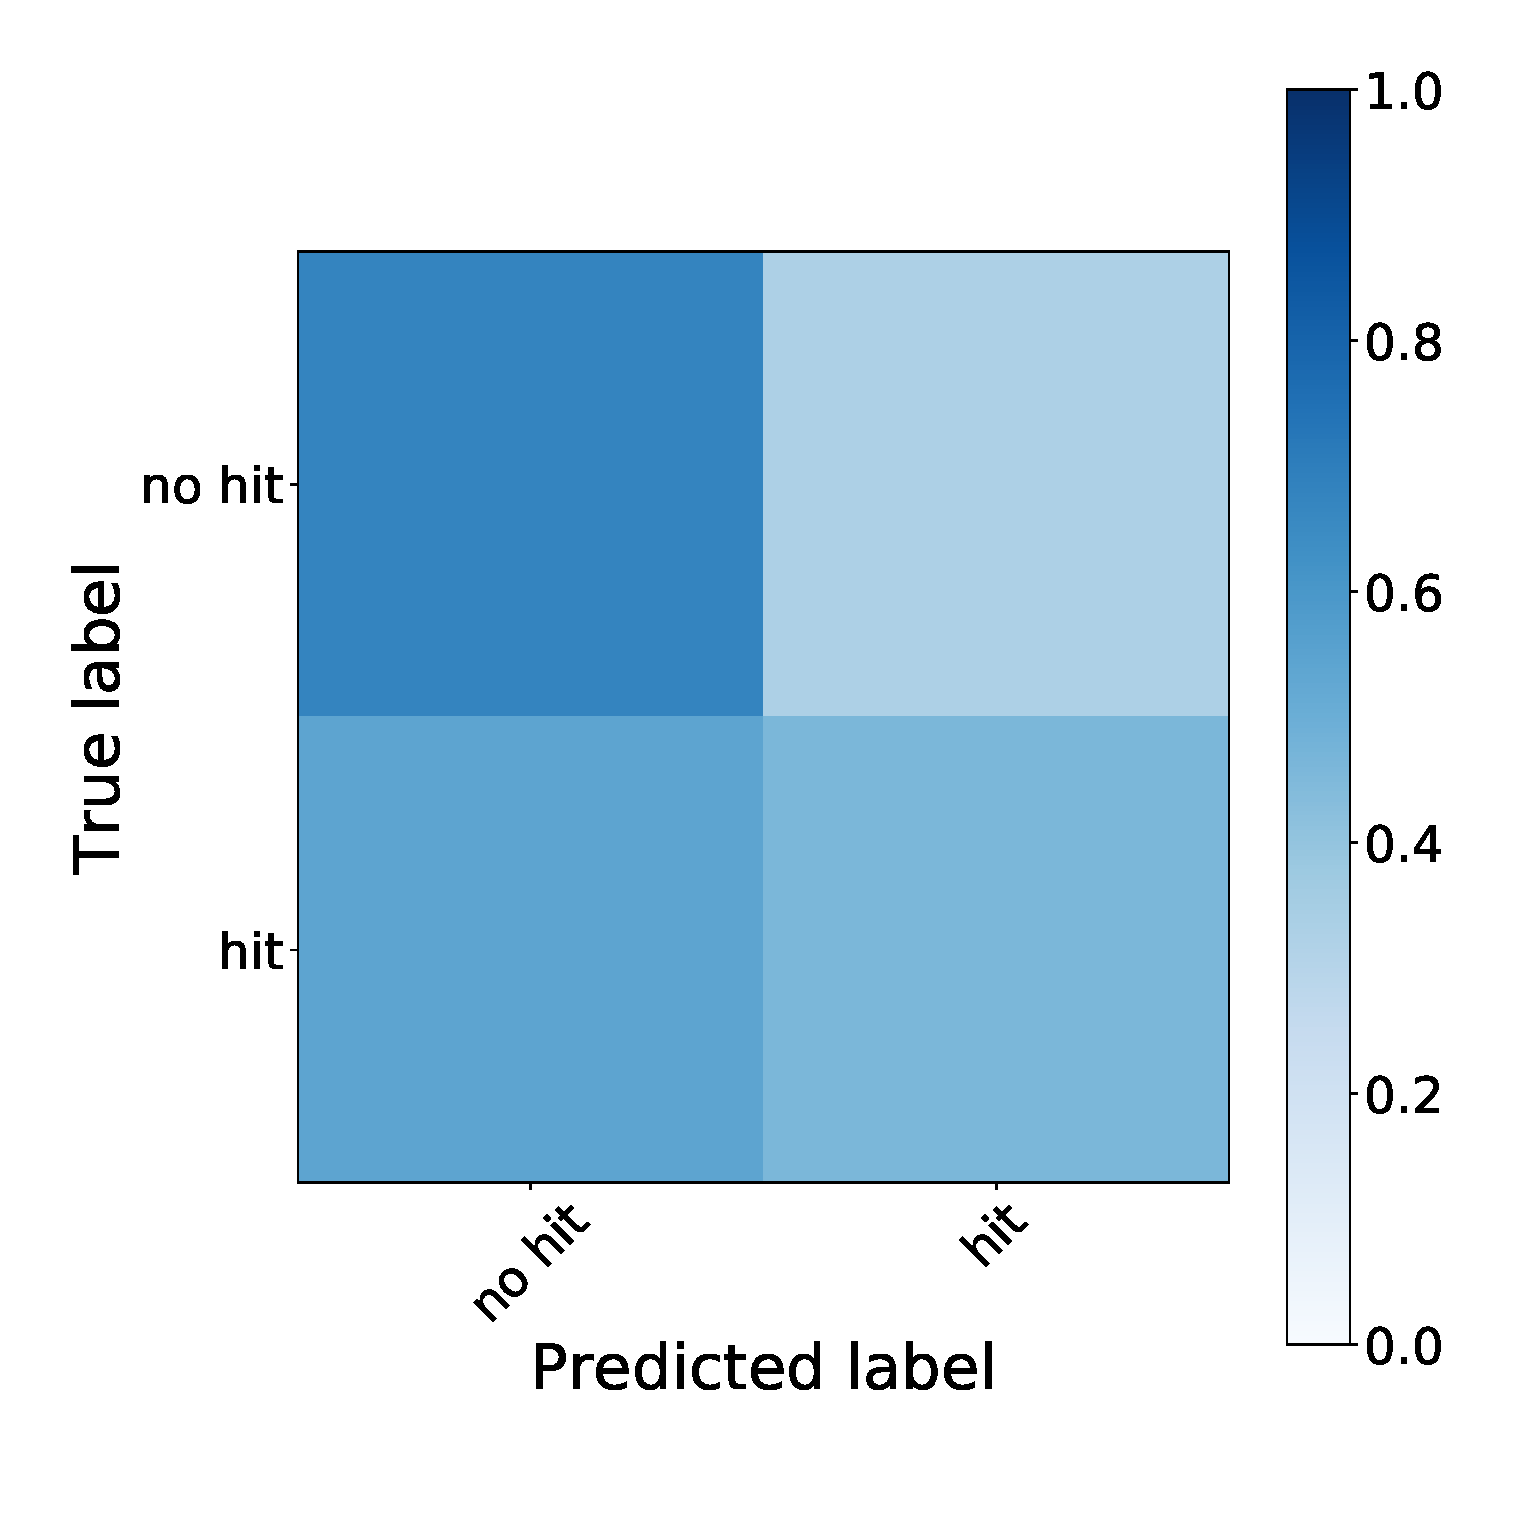
\includegraphics[scale=0.14]{revisedimages/matrix_1.eps}
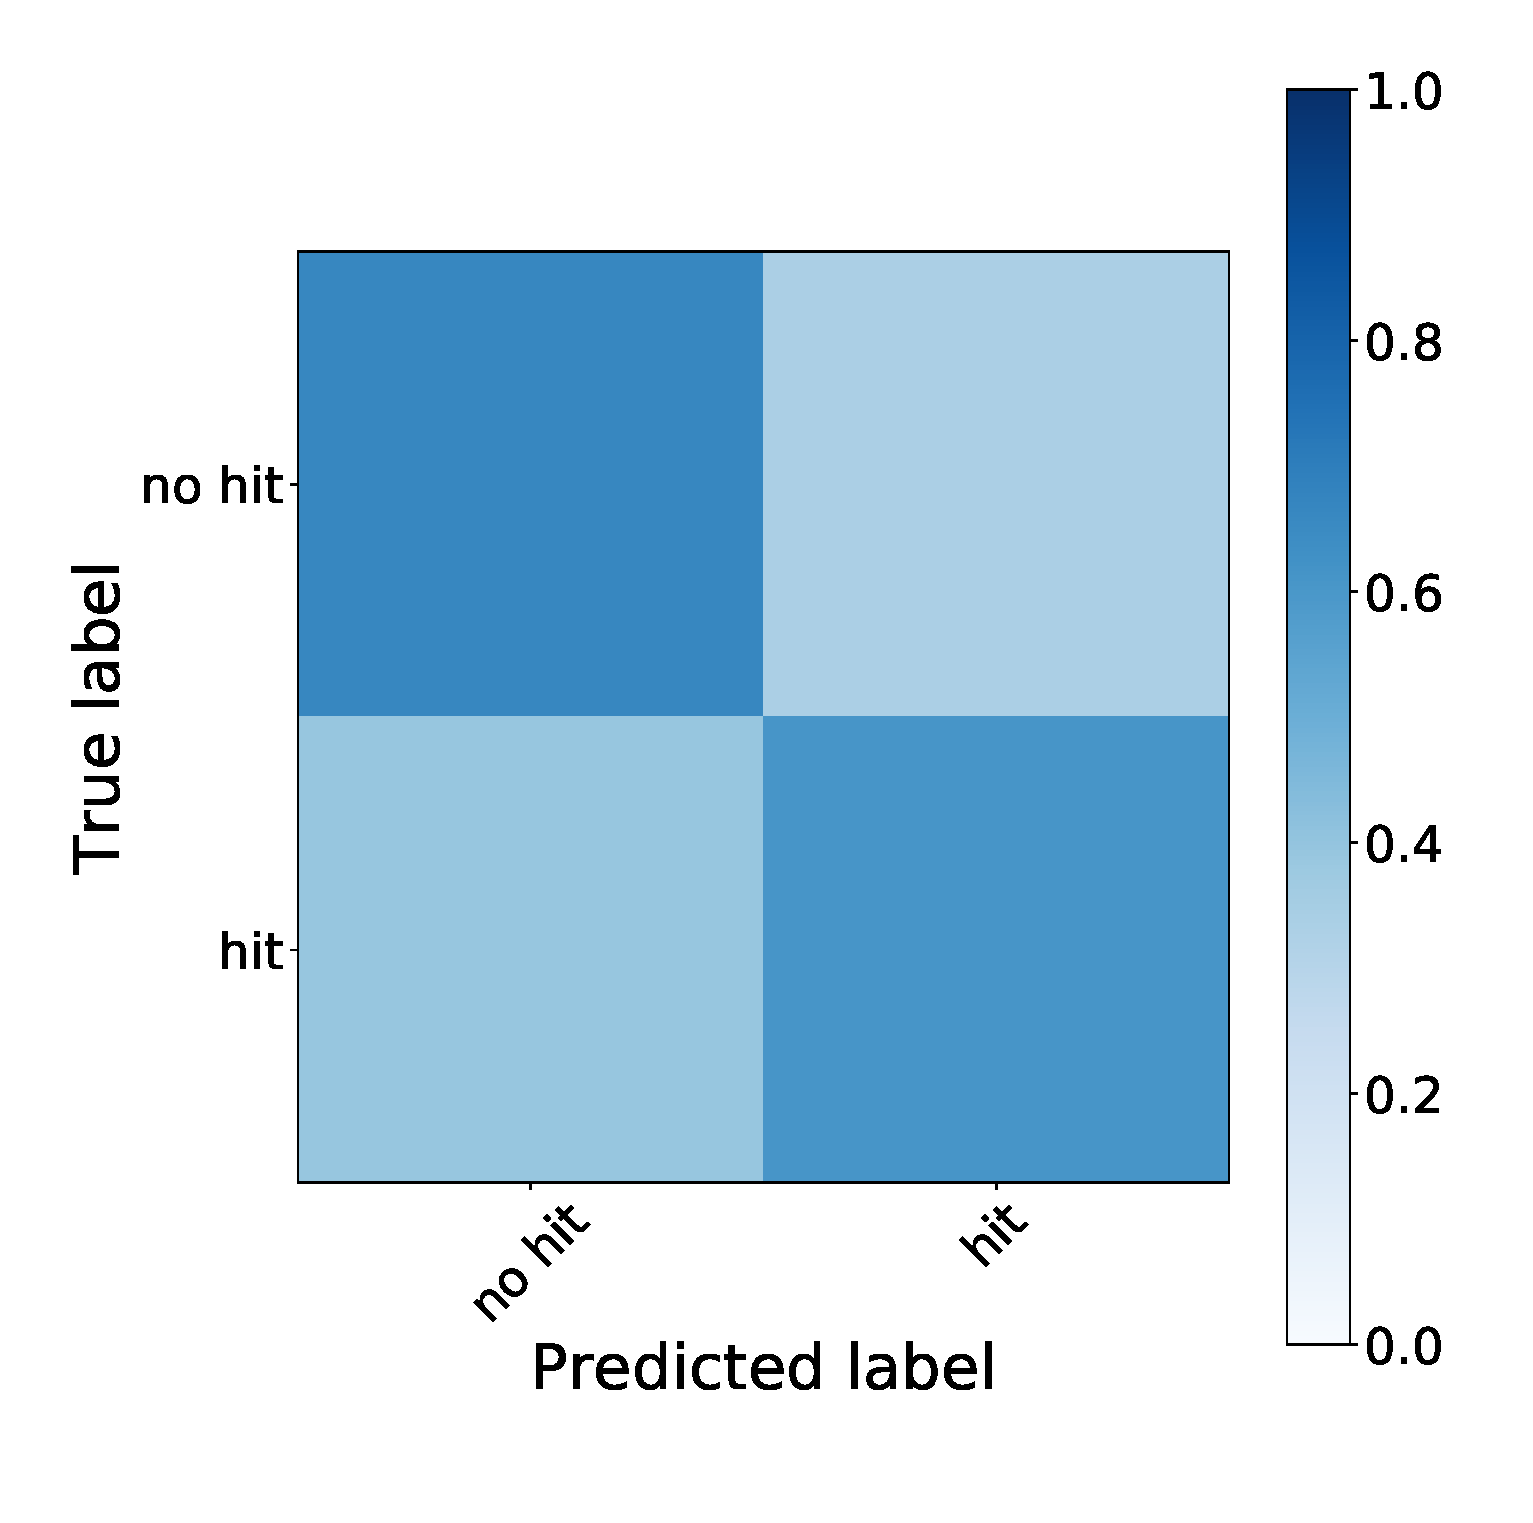
\includegraphics[scale=0.14]{revisedimages/matrix_2.eps}\\
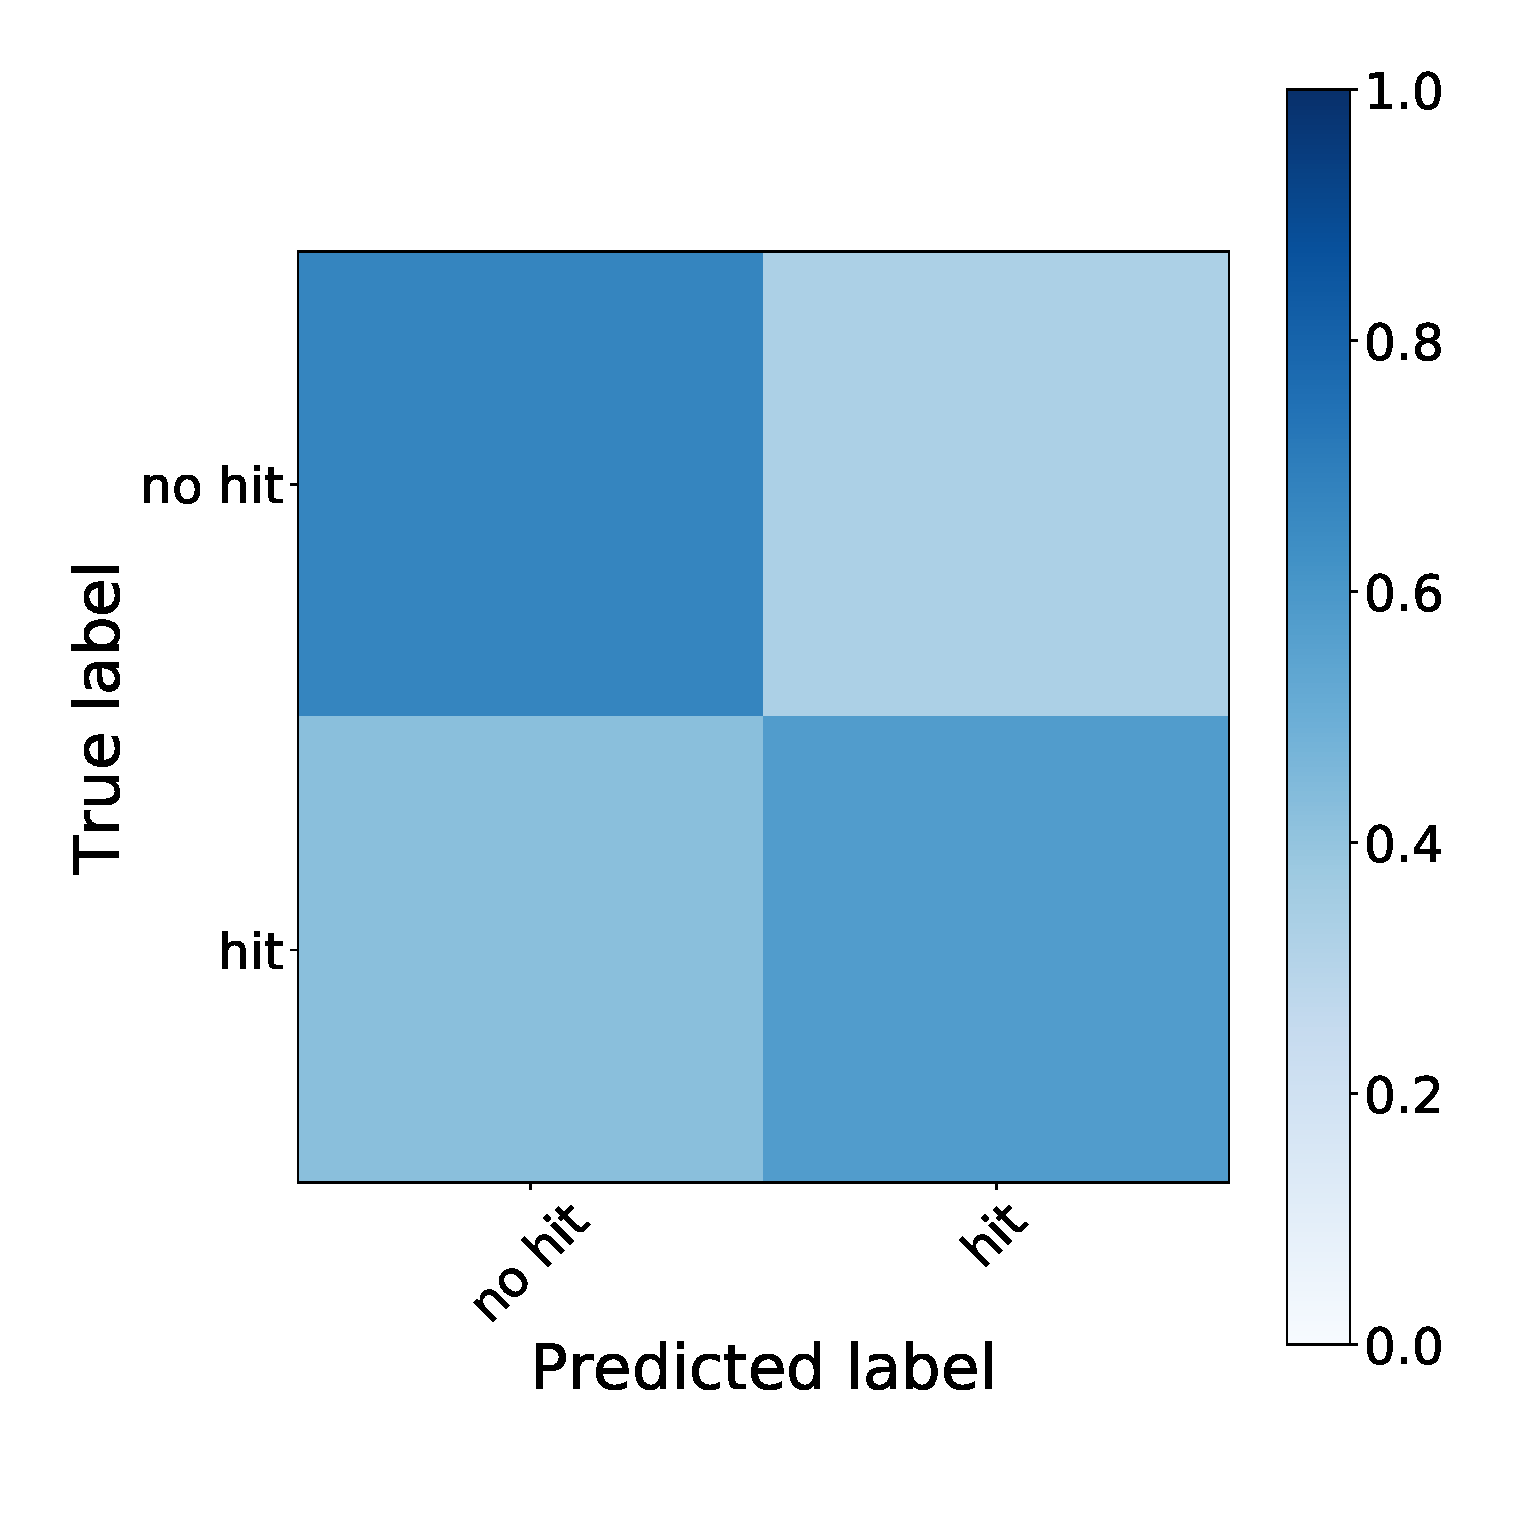
\includegraphics[scale=0.14]{revisedimages/matrix_3.eps}
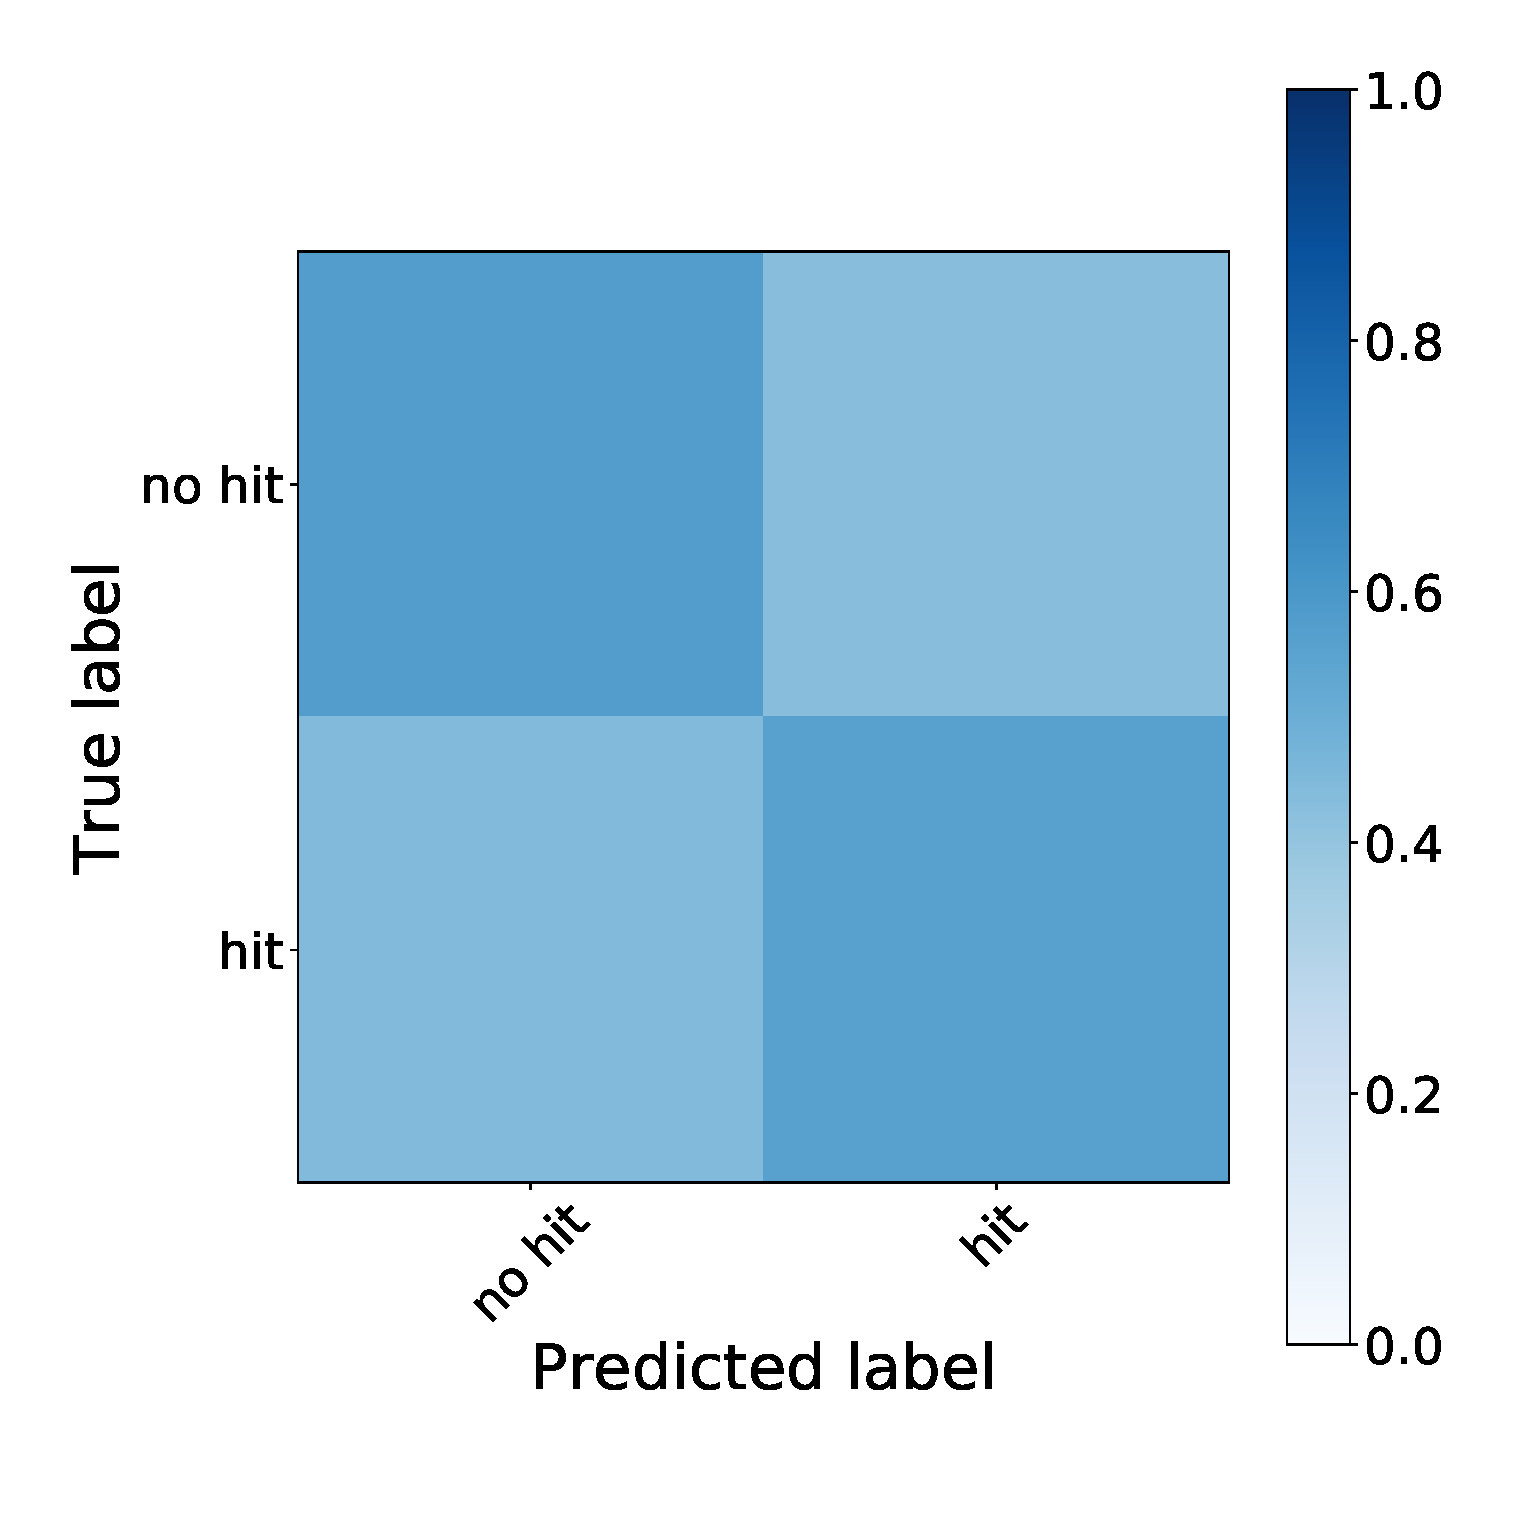
\includegraphics[scale=0.14]{revisedimages/matrix_4.eps}\\
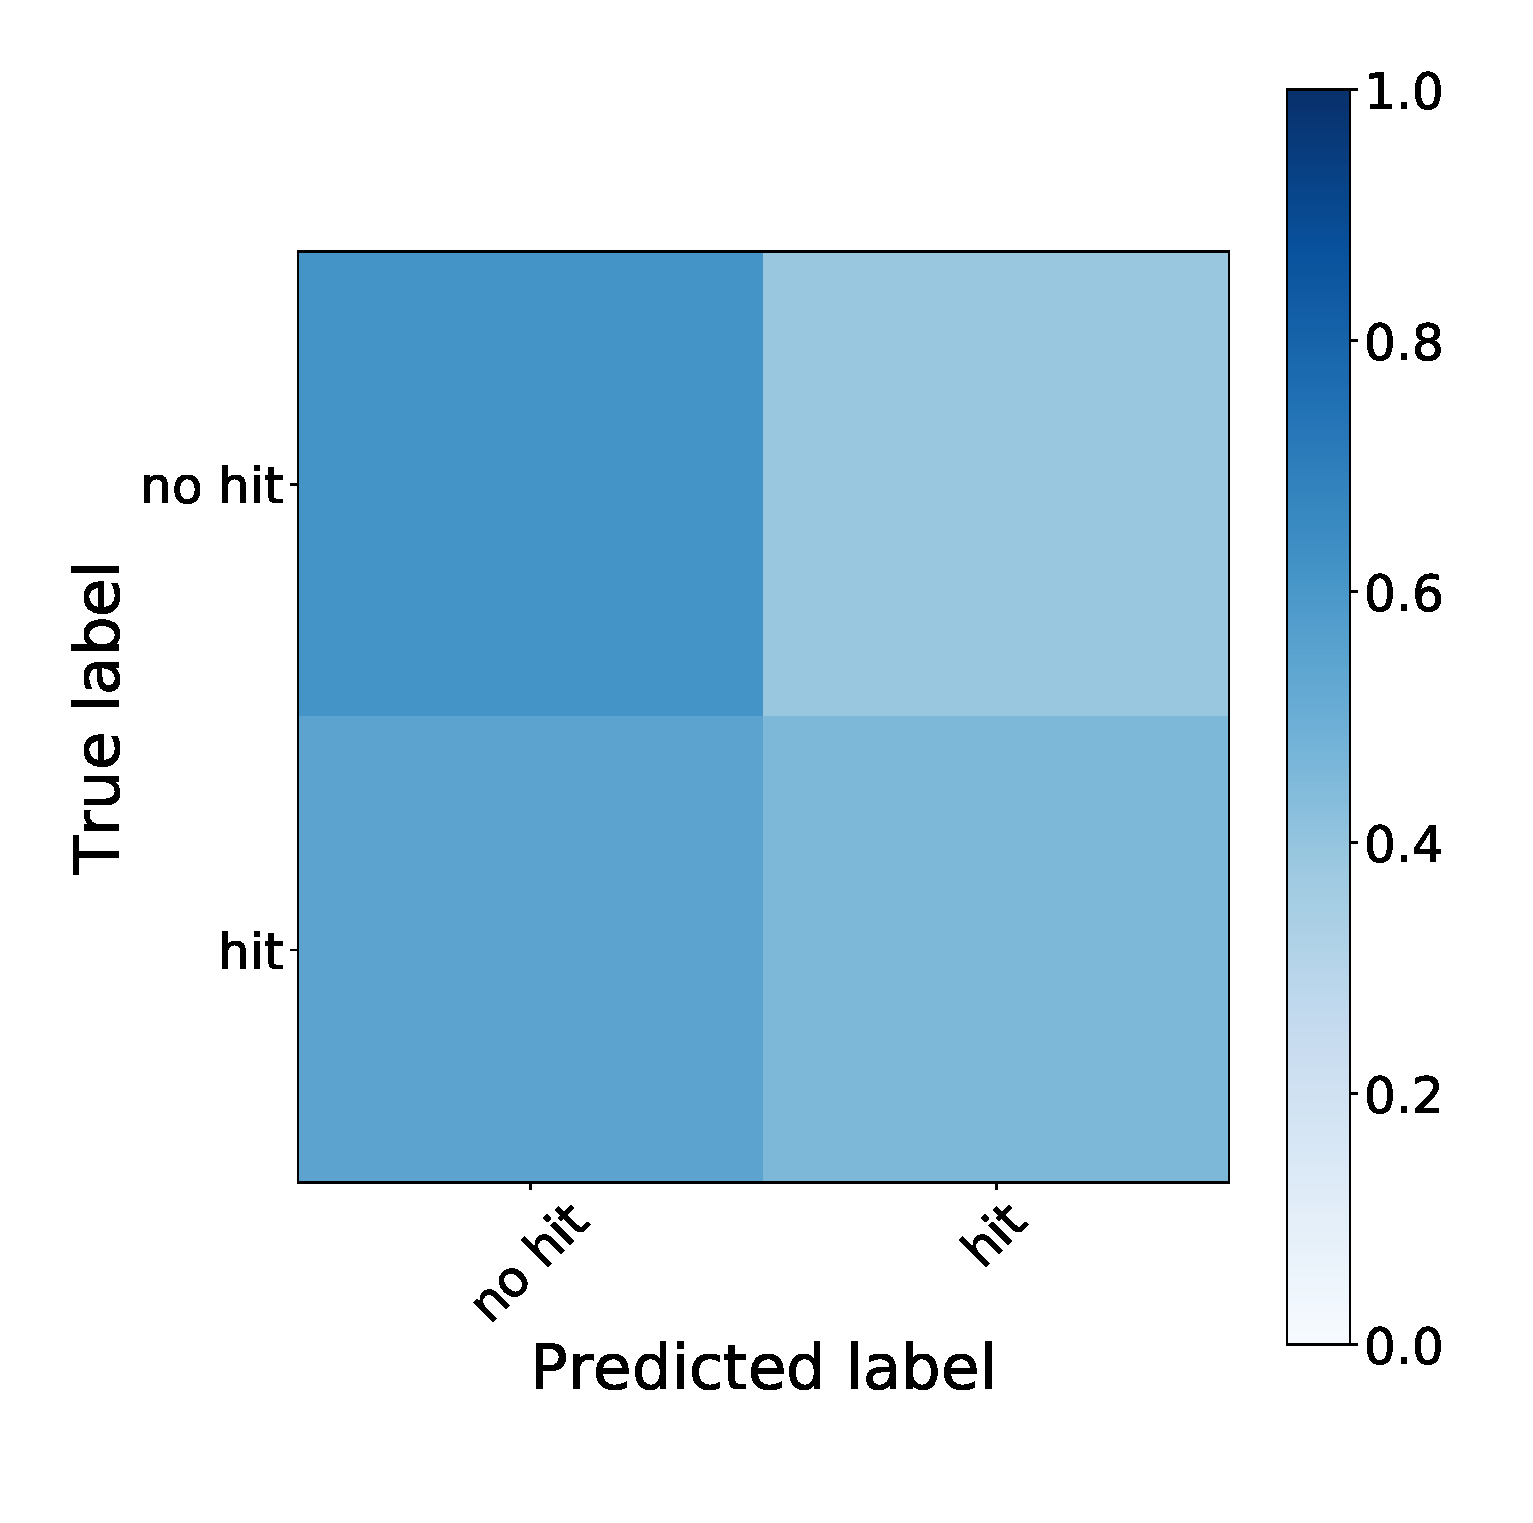
\includegraphics[scale=0.14]{revisedimages/matrix_5.eps}
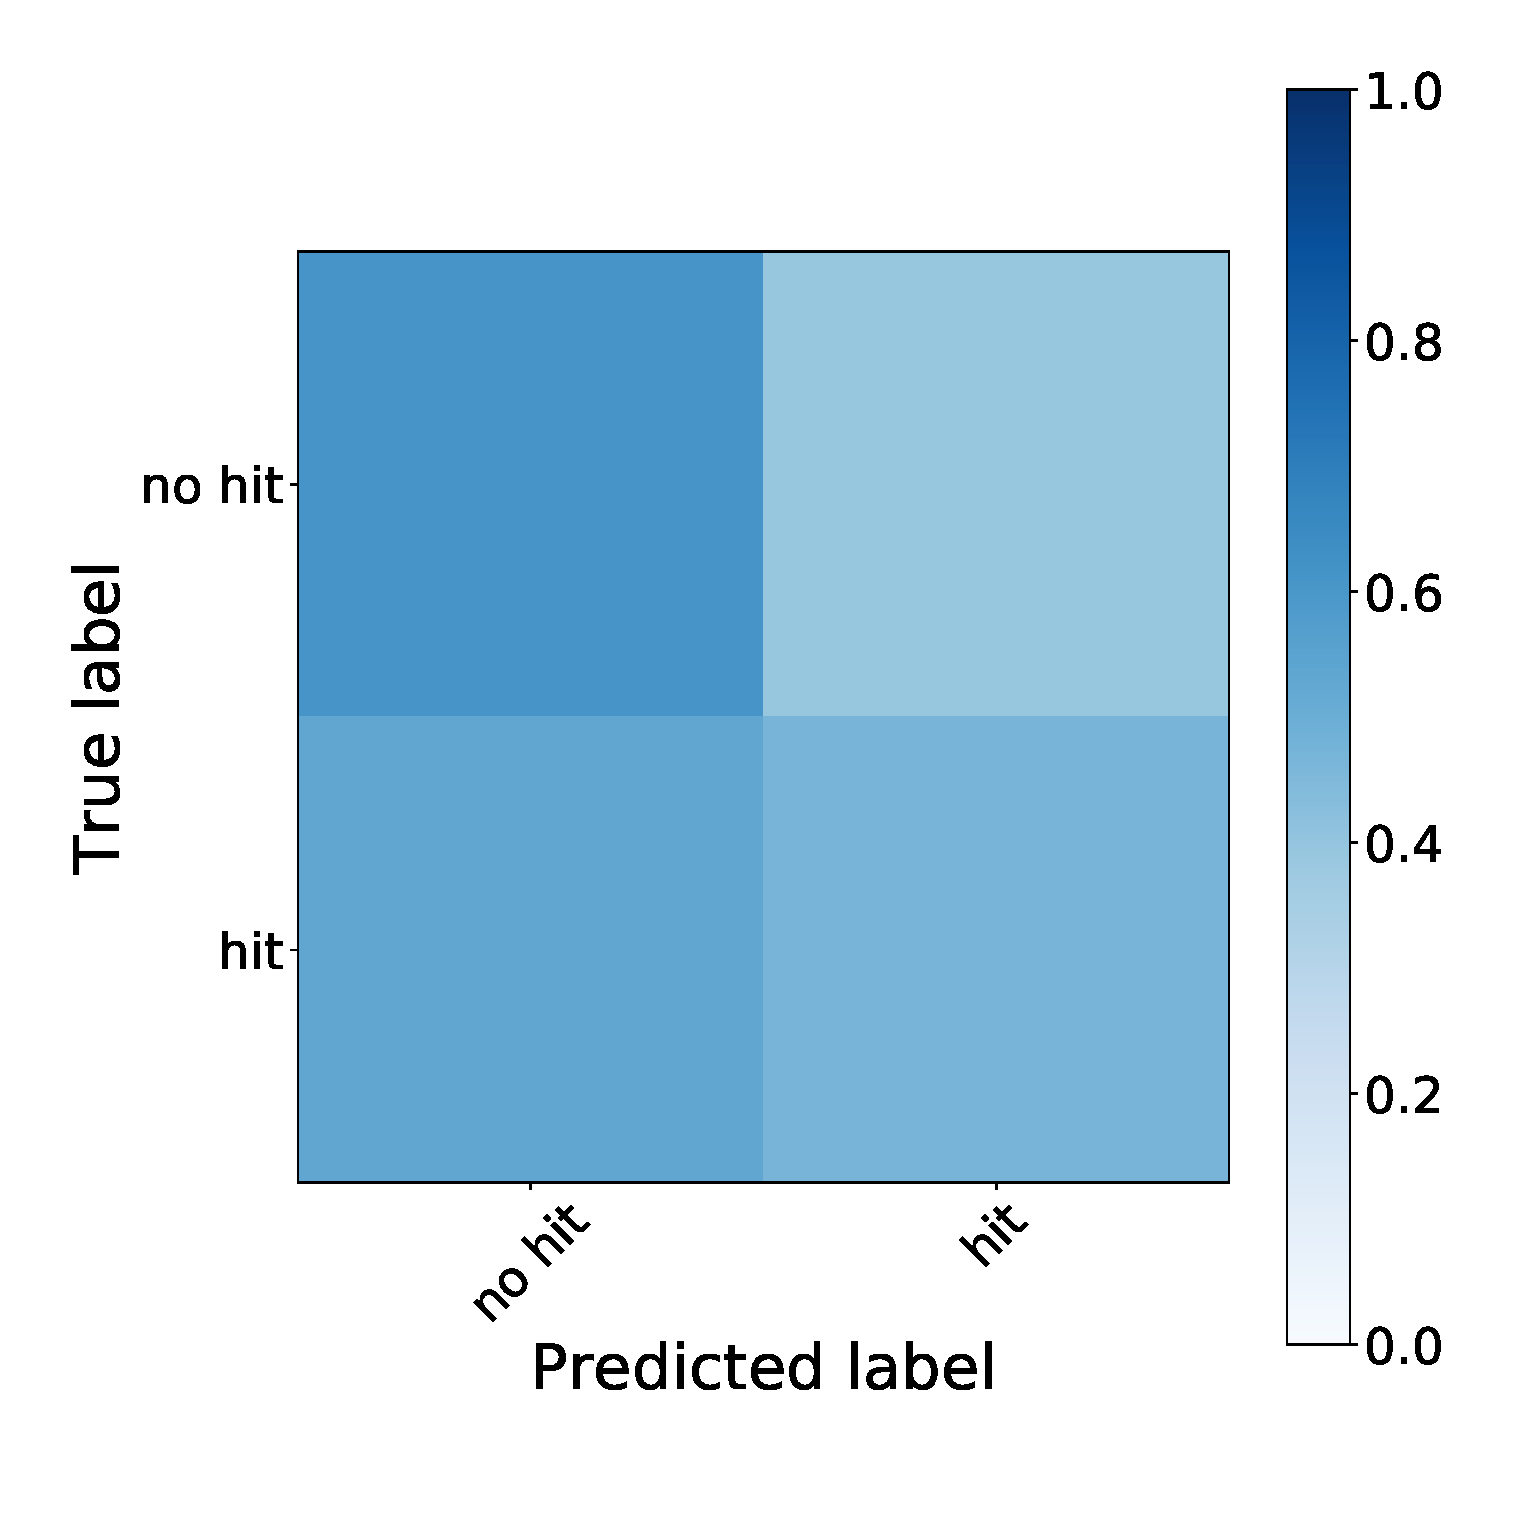
\includegraphics[scale=0.14]{revisedimages/matrix_6.eps}\\
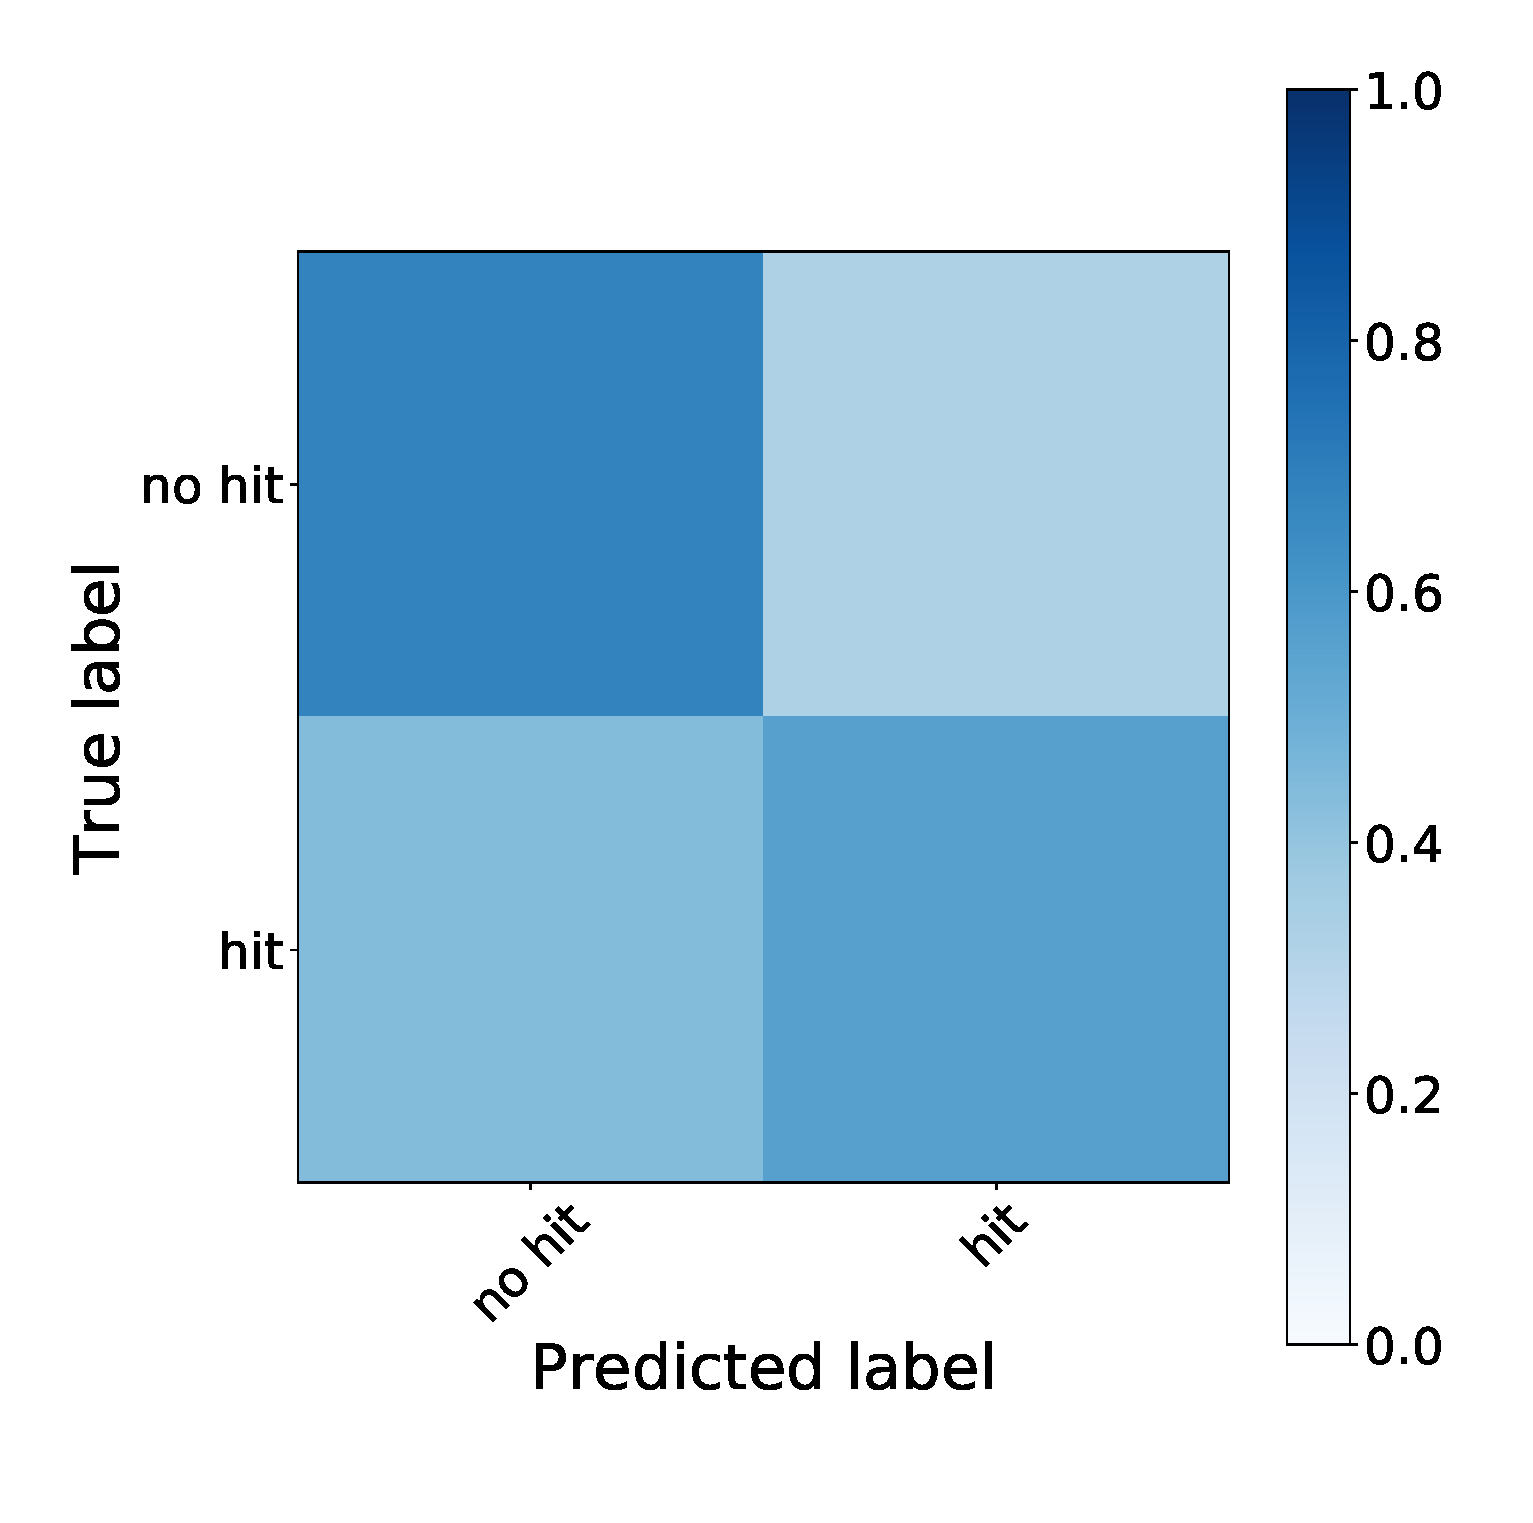
\includegraphics[scale=0.14]{revisedimages/matrix_7.eps}
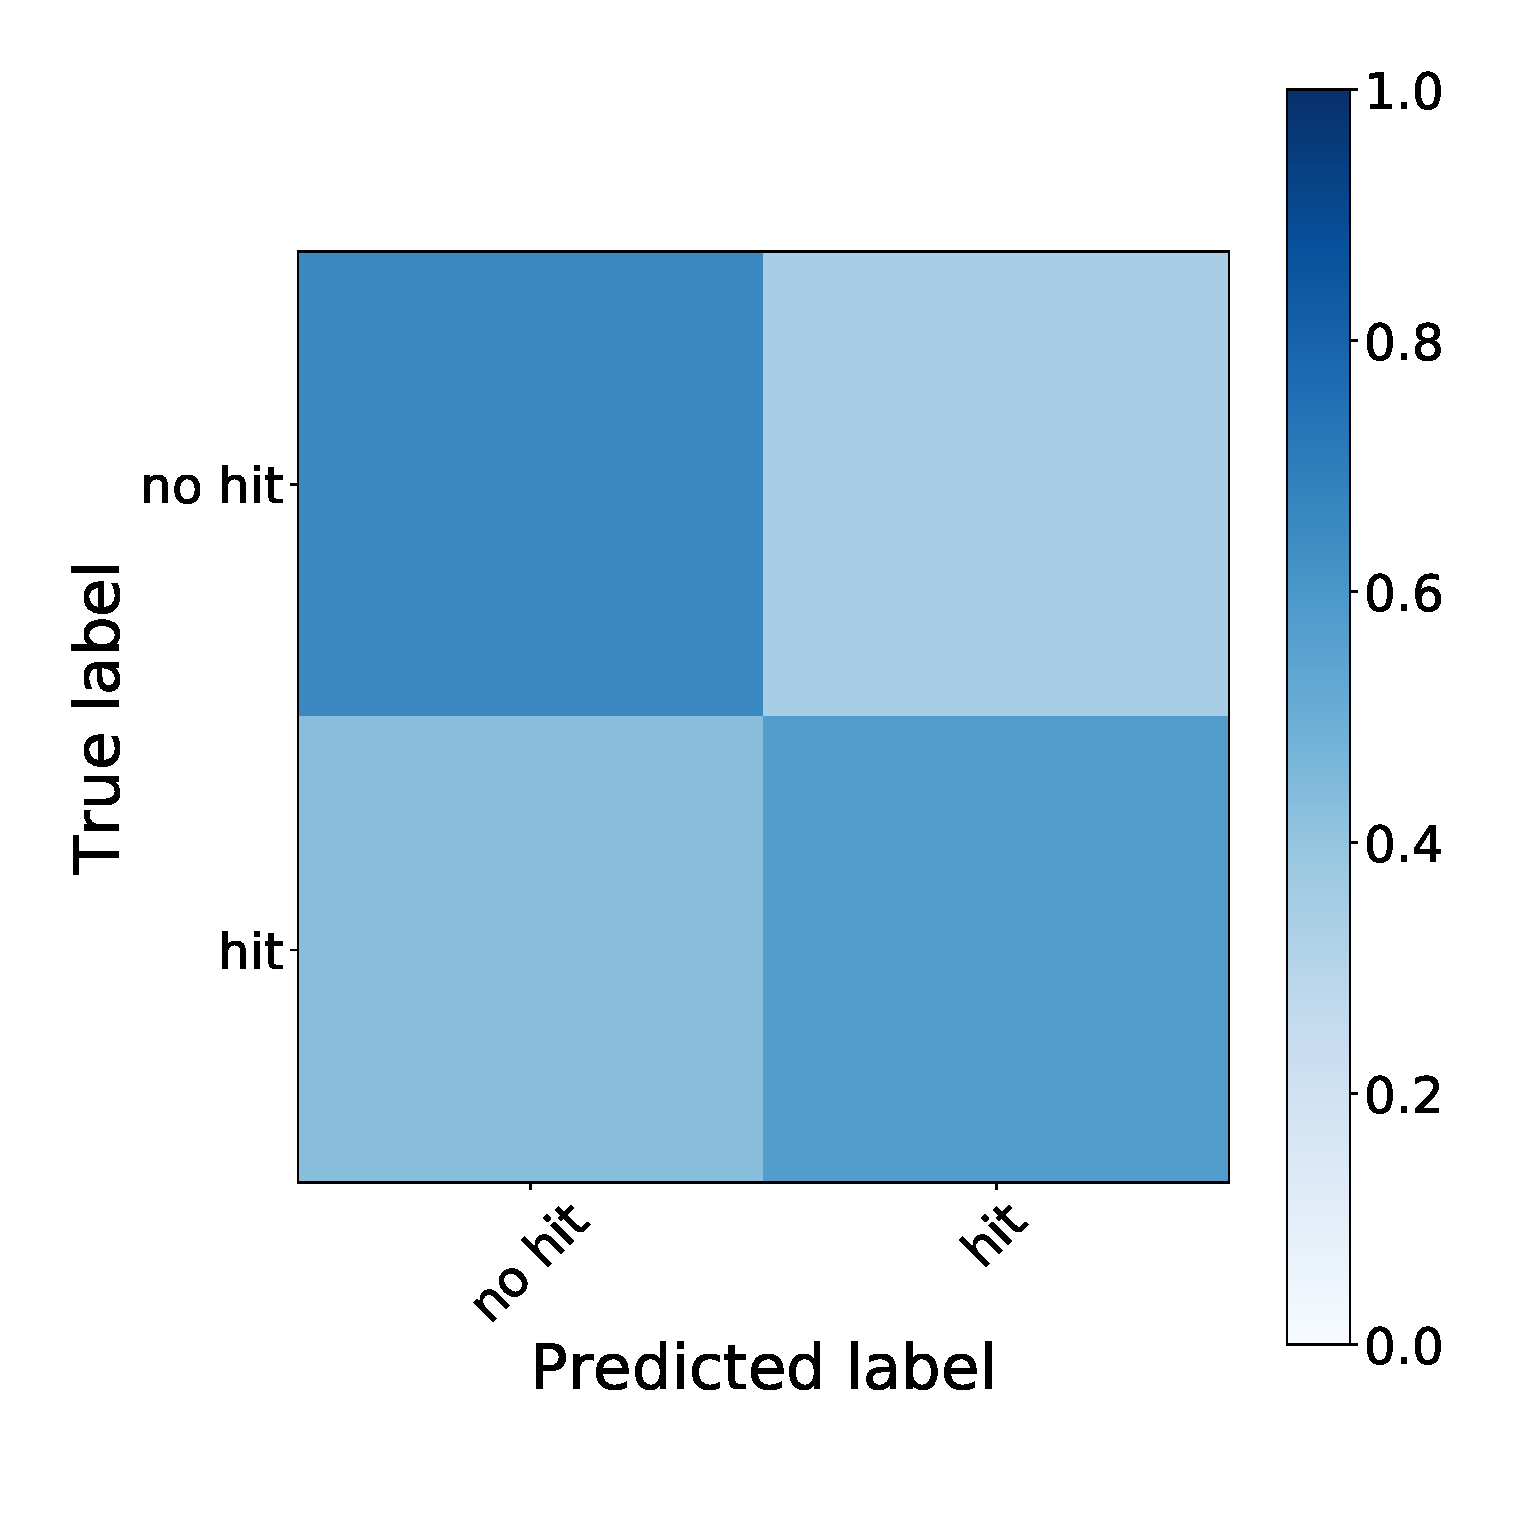
\includegraphics[scale=0.14]{revisedimages/matrix_8.eps}\\
\end{subfigure}
\caption{Confusion Matrix for OHCs 1-8. Darker colors show higher values.  It can be seen the lower percentage of false positives (upper right corner of each chart).}
\label{fig:confusionmatrix}
\end{figure}

%Brainwave sessions have a low amount of matches in order to reduce fatigue from OHCs. However data suggests that longer sessions are required in order to reach better classification scores, since more data are available in order to train the classifier. Matches from OHCs with the largest amounts of data have the best classification scores and produced more accurate rewards. This can also be achieved designing a bigger game system that generates more samples with every session.  While classifying, the better performing classifier is Logistic Regression.

At the same time, effective agent training depends on the OHC's training data. Results confirm the futility or complexity of using Transfer Learning~\cite{Wu2016}: training a classifier with data obtained from one OHC, and using the same classifier to identify ErrPs for another OHC does not increases the performance of the agent.  Despite that, the rewards generated from different subject's classifiers can be used to train the same Q-Table to improve its performance, which may lead to strategies where the overall performance is enhanced based on the information from different human critics at the same time.  There seems to be an agreement in terms of the subjective interpretation of what may be an appropriate movement to reach the goal.

The simple setup of the grid-based game allows further experimentation, using the reduction on the number of average steps to reach the goal as a validation of the achieved information transfer.  It will be of research interest to verify if the smooth progression towards the end alters the shape of the ErrP response, how the ErrP response is triggered in relation with different shapes and colors of the board markers~\cite{EIMER1997143}, or if there is a differential ErrP signal component in relation to up, down, left and right movements.  In addition, the outcome of manipulating the stimulus could be further studied as well as the influence on the results if incentives are given to participants.

Further work will be conducted in order to increase the complexity of the game to allow the possibility that the target position is dynamically changed.  Although we found that the best performing classifier is Logistic Regression, there is room for improvement.  The classifier could be enhanced to recognize the Error Potential~\cite{Iwane2017} more effectively or could be pre-trained to allow higher accuracy~\cite{Spuler2012}.

%Concluding, this research shows evidence that brain signals can be used as an interface between human and a gaming computer enabling an alternative communication with the system without explicit input from the user.


% if have a single appendix:
%\appendix[Proof of the Zonklar Equations]
% or
%\appendix  % for no appendix heading
% do not use \section anymore after \appendix, only \section*
% is possibly needed

% use appendices with more than one appendix
% then use \section to start each appendix
% you must declare a \section before using any
% \subsection or using \label (\appendices by itself
% starts a section numbered zero.)
%

% use section* for acknowledgment
\section*{Acknowledgment}

The authors would like to thank the Laboratory Centro de Inteligencia Computacional and to ITBA University.

\section*{Funding}
This work was supported by the grant ITBACyT-15 issued by ITBA University.

% Can use something like this to put references on a page
% by themselves when using endfloat and the captionsoff option.
\ifCLASSOPTIONcaptionsoff
  \newpage
\fi



% trigger a \newpage just before the given reference
% number - used to balance the columns on the last page
% adjust value as needed - may need to be readjusted if
% the document is modified later
%\IEEEtriggeratref{8}
% The "triggered" command can be changed if desired:
%\IEEEtriggercmd{\enlargethispage{-5in}}

% references section

% can use a bibliography generated by BibTeX as a .bbl file
% BibTeX documentation can be easily obtained at:
% http://mirror.ctan.org/biblio/bibtex/contrib/doc/
% The IEEEtran BibTeX style support page is at:
% http://www.michaelshell.org/tex/ieeetran/bibtex/
\bibliographystyle{IEEEtran}
\bibliography{References}
%
% <OR> manually copy in the resultant .bbl file
% set second argument of \begin to the number of references
% (used to reserve space for the reference number labels box)
% biography section
%
% If you have an EPS/PDF photo (graphicx package needed) extra braces are
% needed around the contents of the optional argument to biography to prevent
% the LaTeX parser from getting confused when it sees the complicated
% \includegraphics command within an optional argument. (You could create
% your own custom macro containing the \includegraphics command to make things
% simpler here.)
%\begin{IEEEbiography}[{\includegraphics[width=1in,height=1.25in,clip,keepaspectratio]{mshell}}]{Michael Shell}
% or if you just want to reserve a space for a photo:

%\begin{IEEEbiography}{Michael Shell}
%Biography text here.
%\end{IEEEbiography}

% if you will not have a photo at all:
%\begin{IEEEbiographynophoto}{John Doe}
%Biography text here.
%\end{IEEEbiographynophoto}

% insert where needed to balance the two columns on the last page with
% biographies
%\newpage

%\begin{IEEEbiographynophoto}{Jane Doe}
%Biography text here.
%\end{IEEEbiographynophoto}

% You can push biographies down or up by placing
% a \vfill before or after them. The appropriate
% use of \vfill depends on what kind of text is
% on the last page and whether or not the columns
% are being equalized.

%\vfill

% Can be used to pull up biographies so that the bottom of the last one
% is flush with the other column.
%\enlargethispage{-5in}



% that's all folks
\end{document}
